% Options for packages loaded elsewhere
\PassOptionsToPackage{unicode}{hyperref}
\PassOptionsToPackage{hyphens}{url}
\PassOptionsToPackage{dvipsnames,svgnames,x11names}{xcolor}
%
\documentclass[
]{article}

\usepackage{amsmath,amssymb}
\usepackage{iftex}
\ifPDFTeX
  \usepackage[T1]{fontenc}
  \usepackage[utf8]{inputenc}
  \usepackage{textcomp} % provide euro and other symbols
\else % if luatex or xetex
  \usepackage{unicode-math}
  \defaultfontfeatures{Scale=MatchLowercase}
  \defaultfontfeatures[\rmfamily]{Ligatures=TeX,Scale=1}
\fi
\usepackage[]{palatino}
\ifPDFTeX\else  
    % xetex/luatex font selection
\fi
% Use upquote if available, for straight quotes in verbatim environments
\IfFileExists{upquote.sty}{\usepackage{upquote}}{}
\IfFileExists{microtype.sty}{% use microtype if available
  \usepackage[]{microtype}
  \UseMicrotypeSet[protrusion]{basicmath} % disable protrusion for tt fonts
}{}
\makeatletter
\@ifundefined{KOMAClassName}{% if non-KOMA class
  \IfFileExists{parskip.sty}{%
    \usepackage{parskip}
  }{% else
    \setlength{\parindent}{0pt}
    \setlength{\parskip}{6pt plus 2pt minus 1pt}}
}{% if KOMA class
  \KOMAoptions{parskip=half}}
\makeatother
\usepackage{xcolor}
\usepackage[top=40mm,left=45mm,right=45mm,bottom=40mm]{geometry}
\setlength{\emergencystretch}{3em} % prevent overfull lines
\setcounter{secnumdepth}{5}
% Make \paragraph and \subparagraph free-standing
\makeatletter
\ifx\paragraph\undefined\else
  \let\oldparagraph\paragraph
  \renewcommand{\paragraph}{
    \@ifstar
      \xxxParagraphStar
      \xxxParagraphNoStar
  }
  \newcommand{\xxxParagraphStar}[1]{\oldparagraph*{#1}\mbox{}}
  \newcommand{\xxxParagraphNoStar}[1]{\oldparagraph{#1}\mbox{}}
\fi
\ifx\subparagraph\undefined\else
  \let\oldsubparagraph\subparagraph
  \renewcommand{\subparagraph}{
    \@ifstar
      \xxxSubParagraphStar
      \xxxSubParagraphNoStar
  }
  \newcommand{\xxxSubParagraphStar}[1]{\oldsubparagraph*{#1}\mbox{}}
  \newcommand{\xxxSubParagraphNoStar}[1]{\oldsubparagraph{#1}\mbox{}}
\fi
\makeatother


\providecommand{\tightlist}{%
  \setlength{\itemsep}{0pt}\setlength{\parskip}{0pt}}\usepackage{longtable,booktabs,array}
\usepackage{calc} % for calculating minipage widths
% Correct order of tables after \paragraph or \subparagraph
\usepackage{etoolbox}
\makeatletter
\patchcmd\longtable{\par}{\if@noskipsec\mbox{}\fi\par}{}{}
\makeatother
% Allow footnotes in longtable head/foot
\IfFileExists{footnotehyper.sty}{\usepackage{footnotehyper}}{\usepackage{footnote}}
\makesavenoteenv{longtable}
\usepackage{graphicx}
\makeatletter
\def\maxwidth{\ifdim\Gin@nat@width>\linewidth\linewidth\else\Gin@nat@width\fi}
\def\maxheight{\ifdim\Gin@nat@height>\textheight\textheight\else\Gin@nat@height\fi}
\makeatother
% Scale images if necessary, so that they will not overflow the page
% margins by default, and it is still possible to overwrite the defaults
% using explicit options in \includegraphics[width, height, ...]{}
\setkeys{Gin}{width=\maxwidth,height=\maxheight,keepaspectratio}
% Set default figure placement to htbp
\makeatletter
\def\fps@figure{htbp}
\makeatother
% definitions for citeproc citations
\NewDocumentCommand\citeproctext{}{}
\NewDocumentCommand\citeproc{mm}{%
  \begingroup\def\citeproctext{#2}\cite{#1}\endgroup}
\makeatletter
 % allow citations to break across lines
 \let\@cite@ofmt\@firstofone
 % avoid brackets around text for \cite:
 \def\@biblabel#1{}
 \def\@cite#1#2{{#1\if@tempswa , #2\fi}}
\makeatother
\newlength{\cslhangindent}
\setlength{\cslhangindent}{1.5em}
\newlength{\csllabelwidth}
\setlength{\csllabelwidth}{3em}
\newenvironment{CSLReferences}[2] % #1 hanging-indent, #2 entry-spacing
 {\begin{list}{}{%
  \setlength{\itemindent}{0pt}
  \setlength{\leftmargin}{0pt}
  \setlength{\parsep}{0pt}
  % turn on hanging indent if param 1 is 1
  \ifodd #1
   \setlength{\leftmargin}{\cslhangindent}
   \setlength{\itemindent}{-1\cslhangindent}
  \fi
  % set entry spacing
  \setlength{\itemsep}{#2\baselineskip}}}
 {\end{list}}
\usepackage{calc}
\newcommand{\CSLBlock}[1]{\hfill\break\parbox[t]{\linewidth}{\strut\ignorespaces#1\strut}}
\newcommand{\CSLLeftMargin}[1]{\parbox[t]{\csllabelwidth}{\strut#1\strut}}
\newcommand{\CSLRightInline}[1]{\parbox[t]{\linewidth - \csllabelwidth}{\strut#1\strut}}
\newcommand{\CSLIndent}[1]{\hspace{\cslhangindent}#1}

\usepackage[noblocks]{authblk}
\renewcommand*{\Authsep}{, }
\renewcommand*{\Authand}{, }
\renewcommand*{\Authands}{, }
\renewcommand\Affilfont{\small}
\usepackage{amssymb}
\usepackage{booktabs} % Add to your preamble for cleaner table lines
\usepackage{makecell} % Add to your preamble for multi-line cells
\usepackage{tikz}
\usepackage{amsmath}
\usepackage{geometry}



\usetikzlibrary{arrows.meta, shapes.geometric}

%% Define TikZ arrow styles
\newcommand{\starstar}{% 
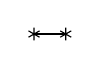
\begin{tikzpicture}[baseline=-3pt]
    \draw [{Rays[n=6]}-{Rays[n=6]}] (0,0) -- (0.55,0);
\end{tikzpicture}
}

\newcommand{\circstar}{% 
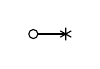
\begin{tikzpicture}
    \draw [{Circle[open]}-{Rays[n=6]}] (0,0) -- (0.55, 0);
\end{tikzpicture}
}

\newcommand{\starcirc}{% 
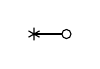
\begin{tikzpicture}
    \draw [{Rays[n=6]}-{Circle[open]}] (0,0) -- (0.55, 0);
\end{tikzpicture}
}

\newcommand{\stararrow}{% 
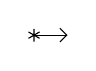
\begin{tikzpicture}
    \draw [{Rays[n=6]}-{Straight Barb[length=2.5pt]}] (0,0) -- (0.5, 0);
\end{tikzpicture}
}

\newcommand{\arrowstar}{% 
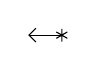
\begin{tikzpicture}
    \draw [{Straight Barb[length=2.5pt]}-{Rays[n=6]}] (0,0) -- (0.5, 0);
\end{tikzpicture}
}

\newcommand{\circarrow}{% 
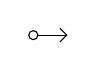
\begin{tikzpicture}
    \draw [{Circle[open]}-{Straight Barb[length=2.5pt]}] (0,0) -- (0.5, 0);
\end{tikzpicture}
}

\newcommand{\tailcirc}{% 
\begin{tikzpicture}[baseline=-3pt] 
    \draw [-{Circle[open]}] (0,0) -- (0.4, 0);
\end{tikzpicture}
}

\newcommand{\circtail}{% 
\begin{tikzpicture}[baseline=-3pt] 
    \draw [{Circle[open]}-] (0,0) -- (0.4, 0);
\end{tikzpicture}
}

\newcommand{\circirc}{% 
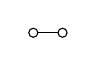
\begin{tikzpicture}[baseline=-3pt] 
    \draw [{Circle[open]}-{Circle[open]}] (0,0) -- (0.5, 0);
\end{tikzpicture}
}

\newcommand{\tailstar}{% 
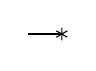
\begin{tikzpicture}[baseline=-3pt] 
    \draw [-{Rays[n=6]}] (0,0) -- (0.5, 0);
\end{tikzpicture}
}

\newcommand{\startail}{% 
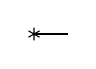
\begin{tikzpicture}
    \draw [{Rays[n=6]}-] (0,0) -- (0.5, 0);
\end{tikzpicture}
}

\newcommand{\tailarrow}{% 
\begin{tikzpicture}
    \draw [-{Straight Barb[length=2.5pt]}](0,0) -- (0.4, 0);
\end{tikzpicture}
}

\newcommand{\arrowtail}{% 
\begin{tikzpicture}
    \draw [{Straight Barb[length=2.5pt]}-](0,0) -- (0.4, 0);
\end{tikzpicture}
}

\newcommand{\arrowarrow}{% 
\begin{tikzpicture}
    \draw [{Straight Barb[length=2.5pt]}-{Straight Barb[length=2.5pt]}](0,0) -- (0.4, 0);
\end{tikzpicture}
}

\newcommand\stackedarrows{%
        \mathrel{\vcenter{\mathsurround0pt
                \ialign{##\crcr
                \noalign{\nointerlineskip}$\arrowtail$\crcr
                \noalign{\nointerlineskip}$\tailarrow$\crcr
                }
        }}%
}
\makeatletter
\@ifpackageloaded{caption}{}{\usepackage{caption}}
\AtBeginDocument{%
\ifdefined\contentsname
  \renewcommand*\contentsname{Table of contents}
\else
  \newcommand\contentsname{Table of contents}
\fi
\ifdefined\listfigurename
  \renewcommand*\listfigurename{List of Figures}
\else
  \newcommand\listfigurename{List of Figures}
\fi
\ifdefined\listtablename
  \renewcommand*\listtablename{List of Tables}
\else
  \newcommand\listtablename{List of Tables}
\fi
\ifdefined\figurename
  \renewcommand*\figurename{Figure}
\else
  \newcommand\figurename{Figure}
\fi
\ifdefined\tablename
  \renewcommand*\tablename{Table}
\else
  \newcommand\tablename{Table}
\fi
}
\@ifpackageloaded{float}{}{\usepackage{float}}
\floatstyle{ruled}
\@ifundefined{c@chapter}{\newfloat{codelisting}{h}{lop}}{\newfloat{codelisting}{h}{lop}[chapter]}
\floatname{codelisting}{Listing}
\newcommand*\listoflistings{\listof{codelisting}{List of Listings}}
\makeatother
\makeatletter
\makeatother
\makeatletter
\@ifpackageloaded{caption}{}{\usepackage{caption}}
\@ifpackageloaded{subcaption}{}{\usepackage{subcaption}}
\makeatother

\ifLuaTeX
  \usepackage{selnolig}  % disable illegal ligatures
\fi
\usepackage{bookmark}

\IfFileExists{xurl.sty}{\usepackage{xurl}}{} % add URL line breaks if available
\urlstyle{same} % disable monospaced font for URLs
\hypersetup{
  pdftitle={From Causal Discovery to Intervention Simulation: Modeling Precariousness and Depression in the HELIUS Study},
  pdfauthor={Kyuri Park ; Leonie K. Elsenburg; Mary Nicolaou; Karien Stronks; Vítor V. Vasconcelos},
  colorlinks=true,
  linkcolor={blue},
  filecolor={Maroon},
  citecolor={Blue},
  urlcolor={Blue},
  pdfcreator={LaTeX via pandoc}}


\title{From Causal Discovery to Intervention Simulation: Modeling
Precariousness and Depression in the HELIUS Study}


\author[1]{%
  Kyuri Park
\thanks{To whom correspondence should be addressed. \url{k.park@uva.nl}}%
  %
}
\author[2]{%
  Leonie K. Elsenburg%
  %
}
\author[2]{%
  Mary Nicolaou%
  %
}
\author[2]{%
  Karien Stronks%
  %
}
\author[1, 3]{%
  Vítor V. Vasconcelos%
  %
}

\affil[1]{\textit{Computational Science Lab, Informatics Institute, University of Amsterdam, PO Box 94323, Amsterdam, 1090GH, the Netherlands}}
\affil[2]{\textit{Department of Public and Occupational Health, Amsterdam Public Health Research Institute, Amsterdam UMC, University of Amsterdam, Amsterdam, the Netherland}}
\affil[3]{\textit{Institute for Advanced Study, University of Amsterdam, Oude Turfmarkt 147, Amsterdam, 1012GC, the Netherland}}

\date{2025-08-25}




\begin{document}
\maketitle
\begin{abstract}
\noindent This study investigates how the internal structure of
depression--precariousness dynamics shapes responsiveness to external
support. Using cross-sectional data from the HELIUS study, we first
apply cycle-capable causal discovery algorithms to estimate directional
dependencies between financial stress, domain-specific precariousness,
and depressive symptoms. Our multi-resolution analysis---spanning both
aggregate and symptom-level constructs---highlights financial stress as
a plausible upstream driver of depression, with symptoms such as sleep
disturbance and depressed mood emerging as initiators of broader social
vulnerability. To translate these structural insights into dynamic
predictions, we construct a family of analytically calibrated linear
stochastic models. Simulations reveal that variations in internal
structure can substantially alter system responses to financial stress
reduction. Some models show rapid but transient improvements in
depression, while others adjust more slowly yet sustain gains over time.
Precariousness tends to respond more immediately across all
configurations, though its trajectory also shifts subtly with structural
variation. Together, these findings demonstrate that intervention
outcomes depend not only on the magnitude of external input but also on
latent properties of the system. More broadly, this study illustrates
how combining causal discovery with dynamical modeling supports
principled, simulation-based exploration of intervention
scenarios---grounded in data, yet able to probe counterfactual
structure. This approach offers a scalable framework for diagnosing
hidden system constraints and informing targeted public health
strategies in complex psychosocial domains.
\end{abstract}


\section{Introduction}\label{introduction}

Mental health disorders represent a growing global health concern,
especially in urbanized regions (Gruebner et al., 2017; World Health
Organization, 2022). In 2019, one in eight people worldwide were living
with a mental health condition, with the highest disability-adjusted
life years (DALYs) due to mental and addictive disorders present in
high-income countries such as those in Northern Europe, North America,
and Australia (Rehm \& Shield, 2019; World Health Organization, 2022).
Despite growing awareness, governments have struggled to design
effective responses. Mental health outcomes arise from complex,
multi-level dynamics between the social, economic, and spatial
structures of urban environments---making both diagnosis and
intervention design deeply challenging (Van Der Wal et al., 2021).

Recent work has shifted focus from individual-level vulnerability to
broader social and structural determinants. While high-income nations
show elevated overall DALYs, within-country disparities reveal that
income inequality is a significant predictor of mental health burden
(Rehm \& Shield, 2019). Moreover, precarious working conditions, housing
instability, and neighborhood disadvantage have all been linked to
increased risk of depression and anxiety (Fone et al., 2014; Pevalin et
al., 2017; Rönnblad et al., 2019; Rugulies et al., 2023). This growing
literature highlights that poor mental health is not merely a personal
issue but one rooted in sustained socioeconomic stress and structural
uncertainty.

Building on this, recent studies have introduced the concept of
precariousness as a multidimensional condition characterized by
instability and lack of control across several life domains, including
employment, finances, housing, social relations, and cultural belonging
(Elsenburg et al., 2025; McKee et al., 2017). This broader view reveals
how different forms of insecurity can co-occur and compound, forming an
ecosystem of risk. However, despite growing evidence of association
between precariousness and mental health, a fundamental question remains
unresolved: \emph{How do these factors causally influence one another?}
Most existing studies rely on cross-sectional correlations, leaving open
questions about directionality and feedback. Without stronger causal
insight, it remains difficult to identify priority targets for
intervention or to anticipate and quantify intended and unintended
effects.

This study aims to investigate the causal mechanisms linking
precariousness and depression and how those mechanisms shape system
responses to external intervention. Specifically, we ask: \emph{How does
the internal configuration of the precariousness--depression
relationship affect the outcomes of stress-reducing interventions?} To
answer this, we combine two approaches. First, we use cycle-capable
causal discovery algorithms to infer directional relationships among
domain-specific precariousness factors and depressive symptoms. By
examining both aggregated measures (depression sum score and a composite
precariousness index) and disaggregated variables (individual depressive
symptoms and specific life-domain indicators), we capture broad patterns
of relationship as well as fine-grained causal pathways. Second, we
translate these insights into a computational dynamical model that
simulates how depression and precariousness co-evolve under varying
levels of external stress. This model enables us to probe how system
properties---such as feedback strength and stochastic noise---govern
responsiveness to intervention. When the effects of depression symptoms
onto the social precarity subsystem are weaker than the reverse path,
there is higher sensitivity of depression to intervention, reflecting
both a faster reduction post financial intervention but also quicker
relapse once financial stresses are reestablished. By integrating causal
discovery with dynamic simulation, we demonstrate that intervention
strategies can be tailored to the underlying architecture of
vulnerability.

\section{Methods}\label{methods}

\subsection{Data}\label{data}

We use data from the HELIUS (HEalthy LIfe in an Urban Setting) study
(Snijder et al., 2017; Stronks et al., 2013). It captures the diverse
population of the city of Amsterdam by including the six main ethnic
groups and provides comprehensive health and lifestyle data, including
depressive symptoms as measured by the PHQ-9 (Galenkamp et al., 2017).
To operationalize indicators of precariousness, we draw on the framework
outlined in previous research (Elsenburg et al., 2025) and select a set
of relevant variables. To ensure a robust representation of
precariousness in our causal discovery models, we conducted exploratory
analyses to identify consistent and meaningful data-driven factor
structures. These analyses led to the identification of five distinct
precariousness factors: three reflecting structural
domains---employment, housing, and social relationships---and two
capturing recent life stressors---financial and relational. Each factor
is composed of multiple observed variables, as outlined below.
Additional details on the HELIUS study and the factor extraction process
are provided in the \hyperref[sec-appendix]{Appendix}.

\begin{itemize}
\tightlist
\item
  Employment precariousness: \texttt{emp\_stat} (current employment
  status), \texttt{work\_sit} (nature of work situation).
\item
  Social precariousness: \texttt{soc\_freq} (frequency of social
  contact), \texttt{soc\_adq} (perceived adequacy of social support).
\item
  Housing precariousness: \texttt{nb\_safe} (neighborhood safety),
  \texttt{nb\_res} (access to neighborhood resources), \texttt{nb\_rent}
  ( proportion of rental housing), \texttt{cul\_rec} (availability of
  cultural resources).
\item
  Recent relational stressors: \texttt{frd\_brk12} (experience of a
  friendship breakup), \texttt{conf12} (recent interpersonal or
  relational conflict).
\item
  Recent financial stressors: \texttt{fincri12} (experience of a
  financial crisis), \texttt{inc\_diff} ( difficulty managing household
  income).
\end{itemize}

Following data cleaning and normalization procedures, the analytical
sample comprises 21,628 individuals. In addition to the five identified
precariousness factors, we computed an overall precariousness score by
summing these five factor scores, thereby capturing a composite measure
of accumulated precariousness across domains. Depression is represented
using the PHQ-9 (Kroenke et al., 2001), both as a total sum score and as
individual symptom scores. In the subsequent causal discovery analysis,
we explore the relationship between depression and precariousness using
both aggregated scores and their disaggregated components. See
Figure~\ref{fig-dist} for the overall distributions of the variables
used in the analysis.

\begin{figure}

\centering{

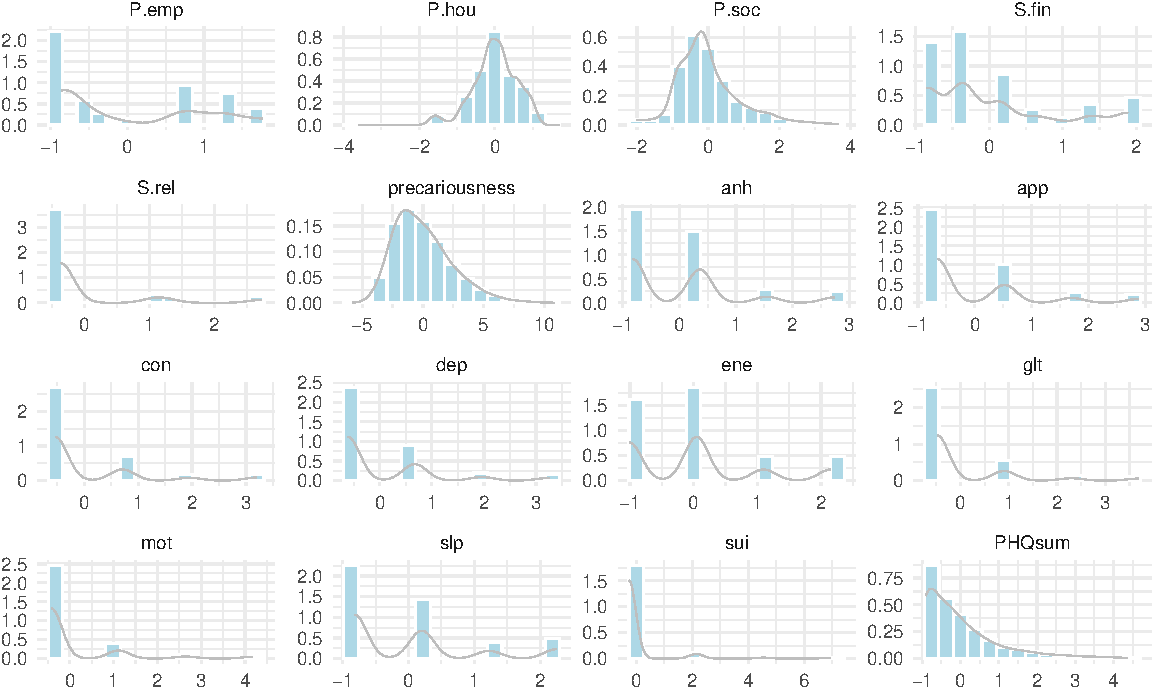
\includegraphics[width=0.9\textwidth,height=\textheight]{draft_v2_files/figure-pdf/fig-dist-1.pdf}

}

\caption{\label{fig-dist}Distributions of variables with density
overlay. \emph{This shows the distributions of the variables used in the
causal analysis, plotted as histograms with overlaid density estimates.
The x-axis represents the value of each variable after preprocessing.
The y-axis shows the corresponding estimated probability density.}
\textbf{\emph{P.emp}} = \emph{employment precariousness};
\textbf{\emph{P.hou}} = \emph{housing precariousness};
\textbf{\emph{P.soc}} = \emph{social precariousness};
\textbf{\emph{S.fin}} = \emph{recent financial stressors};
\textbf{\emph{S.rel}} = \emph{recent relational stressors};
\textbf{\emph{precariousness}} = \emph{overall precariousness};
\textbf{\emph{PHQsum}} = \emph{PHQ-9 sum score}; \textbf{\emph{anh}} =
\emph{anhedonia}; \textbf{\emph{app}} = \emph{appetite};
\textbf{\emph{con}} = \emph{concentration}; \textbf{\emph{dep}} =
\emph{depressed mood}; \textbf{\emph{ene}} = \emph{energy};
\textbf{\emph{glt}} = \emph{guilty}; \textbf{\emph{mot}} = \emph{motor};
\textbf{\emph{slp}} = \emph{sleep}; \textbf{\emph{sui}} =
\emph{suicidal}.}

\end{figure}%

\subsection{Causal Discovery}\label{sec-analysis}

To uncover directional relationships between precariousness and
depression, we use constraint-based causal discovery algorithms that
allow for feedback loops and latent confounding. Specifically, we apply
the \emph{Fast Causal Inference} (FCI) and \emph{Cyclic Causal
Inference} (CCI) algorithms, both of which can detect cycles and
non-acyclic structures (Mooij \& Claassen, 2020; Strobl, 2019). For
reference, we also include the \emph{PC} algorithm, one of the most
widely used methods for acyclic causal discovery (Spirtes et al., 2001).
While our full analysis includes results from three causal discovery
algorithms---FCI, CCI, and PC---we focus on FCI in the main text, as it
offers a strong balance between flexibility and theoretical soundness.
FCI accommodates latent confounding and potential feedback, making it
well-suited for the complexity of our data (Mooij \& Claassen, 2020).
The PC algorithm is included for reference but relies on more
restrictive assumptions, such as acyclicity and no unmeasured
confounding. CCI, while capable of modeling cycles explicitly, has its
own theoretical limitations; for example, its output may not fully
preserve the d-separation properties of the true causal graph (Strobl,
2019). Results from both PC and CCI are provided in the
\hyperref[sec-appendix]{Appendix}
(Section~\ref{sec-cci}, Section~\ref{sec-pc}) for completeness and
comparison. For readers interested in detailed explanations of the
algorithms, edge interpretations, and graph types (e.g., PAG, MAAG,
CPDAG), as well as algorithmic assumptions and limitations, please refer
to the \hyperref[sec-appendix]{Appendix}
(Section~\ref{sec-causalprimer}).

A key challenge in applying these algorithms to the HELIUS dataset is
that many variables are non-Gaussian and likely exhibit nonlinear
relationships. While kernel-based conditional independence tests (such
as KCIT) are well-suited for capturing such complex dependencies, they
are computationally intensive---scaling quadratically with sample size
due to the need to invert large kernel matrices---making them
impractical for large datasets like HELIUS (Rahimi \& Recht, 2007). To
address this, we use the Randomized Conditional Correlation Test (RCoT),
a nonparametric alternative that approximates kernel methods using
random Fourier features. This reduces computational complexity from
quadratic to linear in sample size, substantially lowering runtime while
preserving sensitivity to nonlinear relationships (Strobl et al., 2019;
Zhang et al., 2012). For further details, see Section~\ref{sec-rcot}.

We examine the causal structure using three complementary approaches:

\begin{enumerate}
\def\labelenumi{\arabic{enumi}.}
\tightlist
\item
  Aggregate-level analysis: relationships between five domain-specific
  precariousness factors and the PHQ-9 sum score.
\item
  Fully disaggregated analysis: relationships between individual
  precariousness items and individual depressive symptoms.
\item
  Mixed analysis: relationships between individual symptoms and a
  composite index of overall precariousness.
\end{enumerate}

The aggregate analysis reduces dimensionality and yields interpretable
summaries of how domains of precariousness relate to overall depression
severity. However, it may obscure finer-grained effects. The
disaggregated analysis allows for precise mapping of which symptoms are
influenced by (or influence) specific precariousness conditions, but it
introduces complexity due to the high dimensionality and distributional
properties of the data. The mixed approach, in turn, integrates these
perspectives by examining how individual symptoms respond to cumulative
precariousness across domains.

To robustly estimate the causal structure between depression and
precariousness variables, we implement a comprehensive bootstrapped
causal discovery procedure. This procedure systematically varies key
analysis parameters across a grid of configurations, enabling us to
assess the stability of inferred relationships under different settings.
Specifically, we vary four main components:

\begin{itemize}
\tightlist
\item
  Significance levels for conditional independence tests: \(\alpha\) =
  0.01 and 0.05.
\item
  Stability thresholds: 0.5, 0.6, 0.7, and 0.8, which determine how
  frequently an edge must appear across bootstraps to be retained.
\item
  Conditional independence (CI) tests: Gaussian CI test (partial
  correlation) and RCoT (a nonparametric test).
\item
  Causal discovery algorithms: FCI, CCI, and PC.
\end{itemize}

For each unique parameter combination (2 significance levels × 4
thresholds × 2 CI tests = 16 settings), we run 100 bootstrap samples per
algorithm for the aggregated analyses (see Step 1 in
Figure~\ref{fig-workflow}). For symptom-level analyses, which are more
computationally intensive, we use 30 bootstrap samples per
setting.\footnote{For symptom-level analyses, we further improve
  computational efficiency by fixing the skeleton structure---the
  undirected network of potential connections---using a consensus graph
  derived from all three algorithms (with \(\alpha = 0.01\) and the RCoT
  test). This allows subsequent analyses to focus exclusively on
  estimating edge directions, avoiding the repeated and costly
  computation of skeletons, and thus substantially reducing runtime.}

To summarize these results, we apply a two-level aggregation strategy:

\begin{enumerate}
\def\labelenumi{\arabic{enumi}.}
\tightlist
\item
  \textbf{Within each condition} (fixed \(\alpha\), threshold, CI test,
  and algorithm), we identify the most frequently occurring edge type
  (e.g., arrowhead, circle, none) across bootstraps for each pair of
  variables (Step 2 in Figure~\ref{fig-workflow}).
\item
  \textbf{Across conditions}, we then determine the most dominant edge
  type based on its frequency. In cases where no edge type is clearly
  dominant (i.e., a tie), we mark the edge as uncertain, represented
  with a dashed line in the final graph (Step 3 in
  Figure~\ref{fig-workflow}).
\end{enumerate}

This summarization process is repeated separately for each causal
discovery algorithm (FCI, CCI, PC), yielding a single robust graph per
algorithm. These final graphs represent only the most stable and
consistent relationships across a wide range of plausible
parameterizations, enhancing both reliability and interpretability. To
support transparency, each final graph is accompanied by a matrix
summarizing the relative frequency of each edge type for every variable
pair, enabling readers to assess the degree of uncertainty or agreement
underlying each connection.

\begin{figure}

\centering{

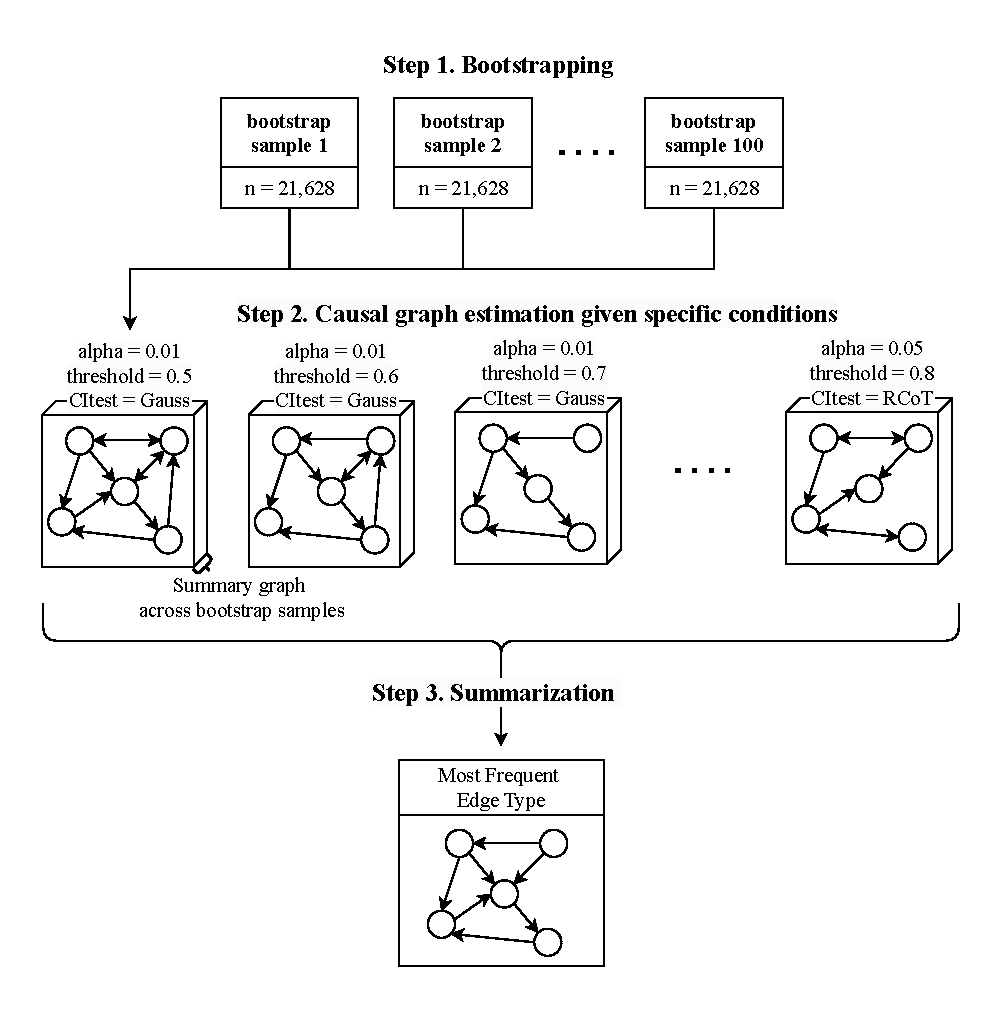
\includegraphics[width=0.9\textwidth,height=\textheight]{img/simsetup.pdf}

}

\caption{\label{fig-workflow}Causal discovery workflow applied across
all three algorithms (FCI, CCI, and PC). \emph{The process involves
three main steps: (1) bootstrapping the dataset to create multiple
resampled datasets; (2) estimating causal graphs under varying parameter
configurations; and (3) summarizing results by identifying the most
frequent edge type across bootstraps and settings to construct a final
stable graph.}}

\end{figure}%

\subsection{Modeling Dynamics between precariousness and
Depression}\label{modeling-dynamics-between-precariousness-and-depression}

To explore how internal system structure shapes responses to external
support, we implement a high-level computational model that formalizes
key mechanisms suggested by the causal discovery analysis. Rather than
attempting to replicate the full estimated causal graph, this model
abstracts the essential structure into a compact, tractable system
focused on dynamic interactions between depression and social
precariousness, both influenced by financial stress.

As illustrated in Figure~\ref{fig-concept}, the model includes three
components: social precariousness \(P_i(t)\), depressive symptoms
\(D_i(t)\), and a static individual-specific external stressor \(S_i\),
representing financial stress. Depression and precariousness are modeled
as coupled state variables that influence each other over time, with
\(S_i\) acting as a shared input. These dynamics are formalized as a
pair of linear stochastic differential equations (SDEs):

\[
\begin{aligned}
dP_i(t) &= \lambda_P \big( \alpha_{PS} S_i + \alpha_{PD} D_i(t) - P_i(t) \big) \, dt + \sigma_P \, dW_{P,i}(t) \\
dD_i(t) &= \lambda_D \big( \alpha_{DS} S_i + \alpha_{DP} P_i(t) - D_i(t) \big) \, dt + \sigma_D \, dW_{D,i}(t)
\end{aligned}
\]

Here, \(D_i(t)\) denotes the depressive state and \(P_i(t)\) denotes the
level of social precariousness for individual \(i\) at time \(t\), with
\(S_i\) representing a static, individual-specific external stressor
(financial stress). The parameters \(\lambda_D\), \(\lambda_P\), as well
as the coefficients \(\alpha\) and noise terms \(\sigma\), are assumed
to be constant across individuals and time. The parameters \(\lambda_D\)
and \(\lambda_P\) govern the timescales over which \(D_i(t)\) and
\(P_i(t)\) adjust toward their respective input-driven target states.
The coefficients \(\alpha_{DS}\) and \(\alpha_{PS}\) quantify the direct
effects of the external stressor \(S_i\) on depression and
precariousness, respectively, while \(\alpha_{DP}\) and \(\alpha_{PD}\)
capture the mutual influence between the two dynamic processes.
Stochastic fluctuations are introduced via the independent Wiener
processes \(dW_{D,i}(t)\) and \(dW_{P,i}(t)\), scaled by their
respective volatility parameters \(\sigma_D\) and \(\sigma_P\). This
linear structure offers a transparent and analytically tractable
framework for modeling how exogenous variation in financial stress may
propagate through individual dynamics of depression and precariousness.
Crucially, all parameters can be calibrated directly from empirical
covariances and variances observed in the HELIUS cohort. The resulting
steady-state distribution of the model aligns with empirical measures:
PHQ-9 total score (PHQsum) for depression, and the derived social
precariousness factor (P.soc) for social precarity. The full calibration
procedure is described in Section~\ref{sec-calibration}.

\begin{figure}

\centering{

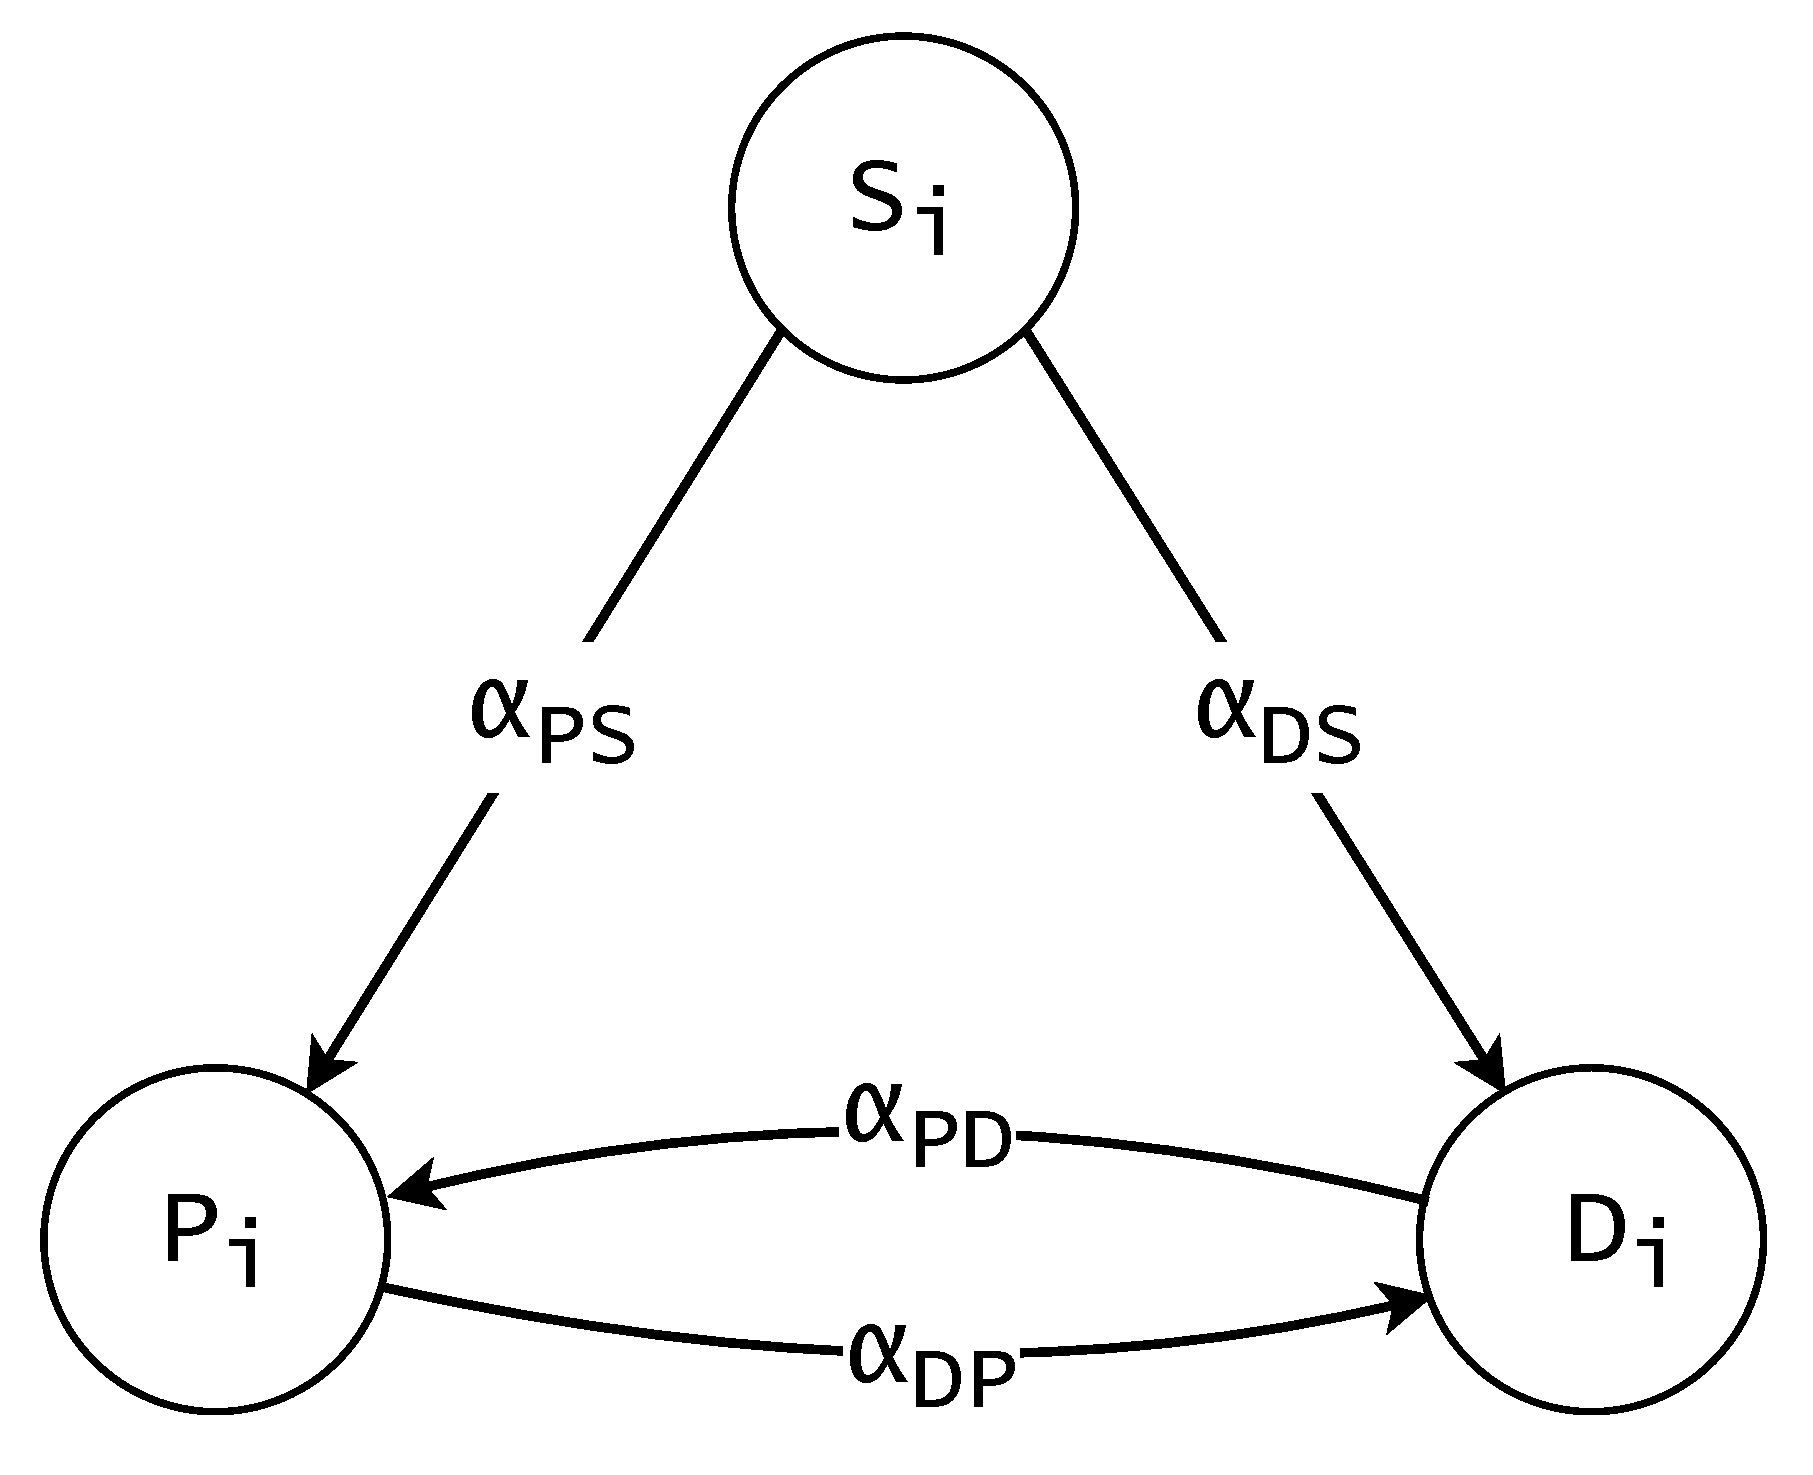
\includegraphics[width=0.4\textwidth,height=\textheight]{img/conceptmodel.pdf}

}

\caption{\label{fig-concept}High-level schematic of the dynamic model
structure used in simulation. Arrows represent influence coefficients
\(\alpha\), matching the terms in the system of stochastic differential
equations. \(D_i(t)\) and \(P_i(t)\) denote depressive symptoms and
social precariousness for individual \(i\), with \(S_i\) representing
static financial stress.}

\end{figure}%

\subsubsection{Model Calibration}\label{sec-calibration}

In our linear model, all parameters are derived analytically to
reproduce the empirical second-order moments observed in the HELIUS
dataset. The system treats depression (\(D\)) and social precariousness
(\(P\)) as jointly evolving under the influence of a shared external
stressor (\(S\)), forming a coupled system of Ornstein--Uhlenbeck
processes. Under the assumption of stationarity, the steady-state
covariances between these variables admit closed-form solutions for the
system's structural parameters.

We fix the adjustment rates \(\lambda_D = \lambda_P = 1\), which
normalizes the time scale given the cross-sectional nature of the HELIUS
data. To resolve the remaining degree of freedom, we treat the feedback
from precariousness to depression (\(\alpha_{DP}\)) as a free parameter,
and we solve algebraically for all other coefficients --- specifically
the direct effects of stress (\(\alpha_{DS}, \alpha_{PS}\)), the reverse
feedback from depression to precariousness (\(\alpha_{PD}\)), and the
noise terms (\(\sigma_D, \sigma_P\)). These solutions are expressed as
closed-form functions of the empirical covariances: \(\mathrm{Var}(D)\),
\(\mathrm{Var}(P)\), \(\mathrm{Var}(S)\), \(\mathrm{Cov}(D, P)\),
\(\mathrm{Cov}(D, S)\), and \(\mathrm{Cov}(P, S)\).

This structure creates a family of analytically calibrated models, each
consistent with the same observed covariances but differing in their
internal configuration. We constrain the space of valid solutions by
imposing that all structural parameters must be positive, reflecting the
assumption that stress and precariousness contribute adversely to
depression. This constraint restricts the allowable range of
\(\alpha_{DP}\) to approximately \([0, 0.698]\) (see Appendix
Section~\ref{sec-analcalibration}).

Figure~\ref{fig-tradeoff} illustrates how the remaining parameters
adjust as \(\alpha_{DP}\) increases to maintain consistency with the
empirical covariances. As \(\alpha_{DP}\) increases, \(\alpha_{PD}\)
tends to decrease, reflecting a compensatory trade-off between the
mutual influences of depression and precariousness. This interplay helps
preserve the model's match with observed covariances, without requiring
major shifts in external input strength. Meanwhile, the external
coupling terms --- \(\alpha_{DS}\) and \(\alpha_{PS}\) --- also shift to
absorb variance in a way that maintains alignment with the empirical
data. Notably, the noise amplitudes \(\sigma_D\) and \(\sigma_P\)
decline slightly as \(\alpha_{DP}\) increases. This indicates that more
of the observed variability is captured by deterministic interactions,
with less left to be explained by stochastic fluctuations.

Rather than being a limitation, this flexibility enables exploration of
a spectrum of equally data-consistent feedback regimes. Each represents
a different plausible causal architecture, offering insight into how
internal dynamics modulate the system's responsiveness to external
stress --- even when the observed covariances remain unchanged.

\begin{figure}

\centering{

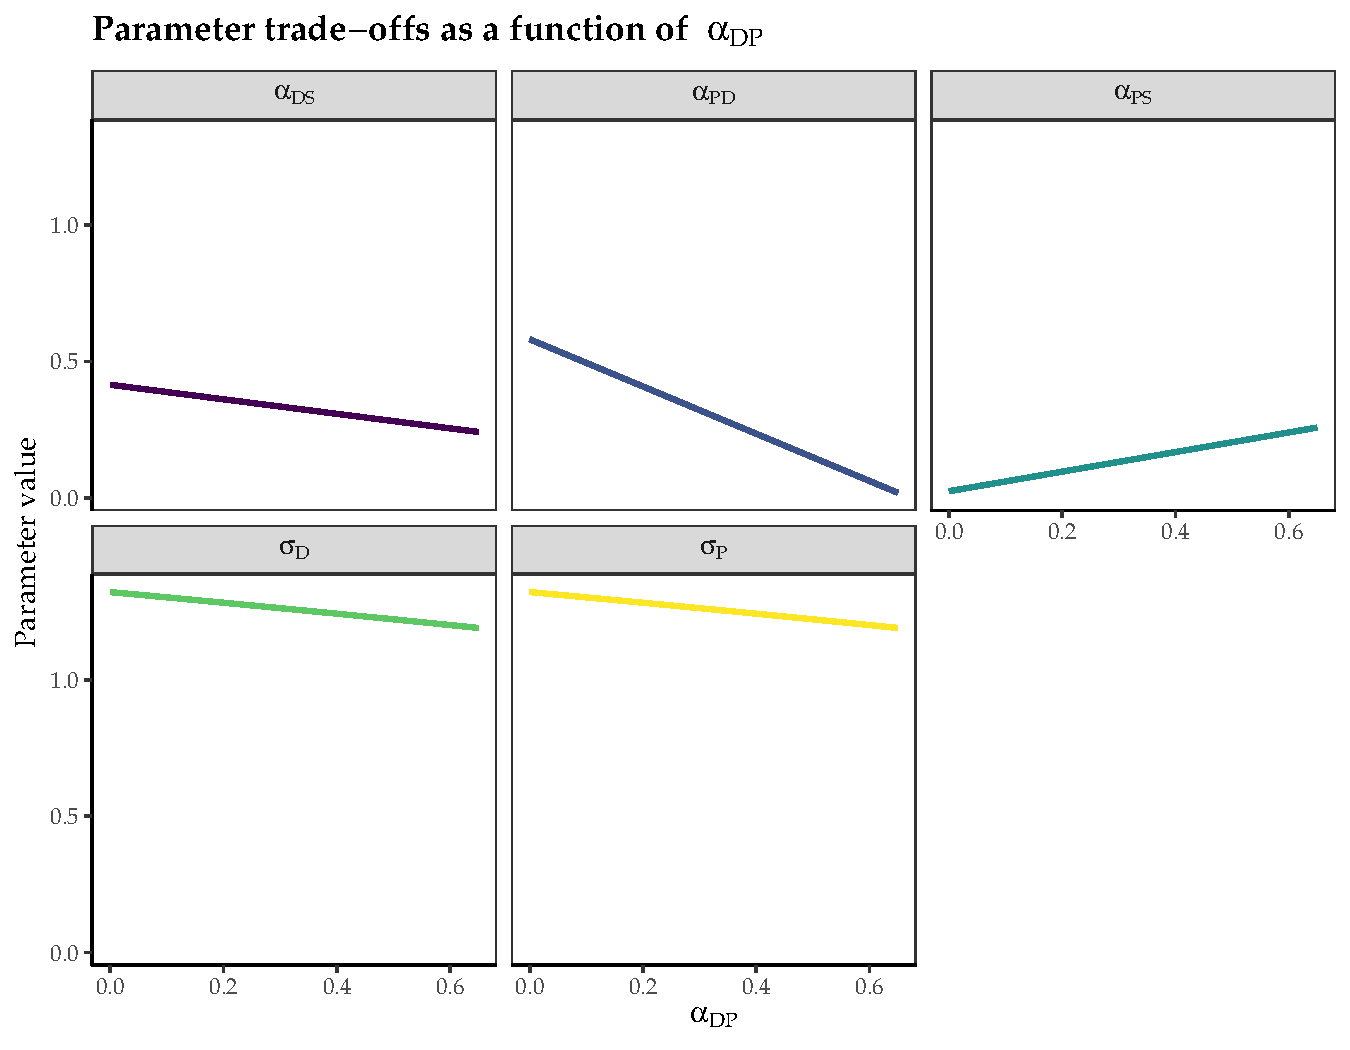
\includegraphics[width=1\textwidth,height=\textheight]{img/param_tradeoff.pdf}

}

\caption{\label{fig-tradeoff}Trade-off curves showing how calibrated
parameters vary with \(\alpha_{DP}\). \emph{Each line shows how a
different parameter adjusts in response to changes in \(\alpha_{DP}\) to
maintain consistency with empirical covariances from the HELIUS data.
All configurations shown are equally consistent with the data,
illustrating how internal dynamics adjust as feedback strength
changes.}}

\end{figure}%

\subsubsection{Intervention Simulation}\label{intervention-simulation}

To evaluate how internal structure affects system responsiveness, we
simulate a family of linear models subjected to external intervention.
Each model corresponds to a different value of \(\alpha_{DP}\),
representing the strength of influence from social precariousness to
depression. The range spans from 0 (no coupling) to 0.65 (maximal
admissible value), with all other parameters derived analytically to
preserve the empirical covariances observed in the HELIUS data (see
Figure~\ref{fig-tradeoff}).

In each simulation, financial stress of individual \(i\) (\(S_i\)) is
proportionally reduced toward the lowest observed value, modeling a
population-wide intervention applied at varying intensities (0--100\%).
For each model, we simulate 1000 virtual individuals whose baseline
stress levels are sampled from the empirical distribution and scaled
according to the intervention level.

We assess the system's behavior using two complementary approaches:

\begin{itemize}
\item
  Snapshot analysis captures the average levels of depression (\(D\))
  and precariousness (\(P\)) at selected time points (\(t = 100\),
  \(300\), \(500\)) following intervention onset. Since all linear
  models converge to the same equilibrium, this highlights how internal
  feedback affects the speed and pathway of adjustment.
\item
  Full trajectory simulation tracks system dynamics over time for two
  representative models: one with minimal (\(\alpha_{DP} = 0\)) and one
  with maximal (\(\alpha_{DP} = 0.65\)) feedback. Each simulation
  includes an intervention period followed by its withdrawal, revealing
  differences in reactivity, delay, and recovery stability.
\end{itemize}

Together, these simulations demonstrate how internal structure governs
not just whether change occurs, but how it unfolds --- shaping the pace,
persistence, and variability of response to external support.

\section{Results}\label{results}

\subsection{Causal Structure Linking Precariousness and
Depression}\label{causal-structure-linking-precariousness-and-depression}

\subsubsection{Depression as sum score}\label{depression-as-sum-score}

Figure~\ref{fig-sum} provides a high-level summary of how precariousness
factors collectively influence and are influenced by overall depression
severity, focusing on the causal relationships between precariousness
factors (\emph{P.hou}, \emph{P.emp}, \emph{P.soc}, \emph{S.rel},
\emph{S.fin}) and the depression sum score (\emph{PHQsum}), as
identified by the FCI algorithm.

In panel (a) we see that employment precariousness (\emph{P.emp}) and
social precariousness (\emph{P.soc}) are not identified as causes of
depression, whereas financial stress (\emph{S.fin}) appears to play a
causal role. While \emph{P.emp} and \emph{P.soc} are generally not
recognized as causes of other precariousness factors, \emph{S.fin}
emerges as a potential cause, as indicated by its circle edge endpoint.
This pattern is further supported by the edge-type proportion matrix
shown in panel (b), which aggregates edge inference outcomes across
bootstrapped datasets.

Relational stress (\emph{S.rel}) plays a more nuanced role, interacting
with depression and \emph{S.fin} through a latent confounder. Its
connection to \emph{P.soc} is less definitive---the proportion matrix in
Figure~\ref{fig-sum-2} suggests that this relationship is frequently
absent, ambiguous, or potentially bidirectional across bootstrap
samples. Meanwhile, housing precariousness (\emph{P.hou}) is not
directly causally related to depression but is linked to \emph{P.emp}
and \emph{S.fin}. While \emph{P.emp} and \emph{S.fin} are identified as
non-causes of \emph{P.hou}, it remains unclear whether \emph{P.hou}
causally influences \emph{P.emp} or if their relationship is mediated by
an unobserved confounder.

The findings from the CCI algorithm (see Figure~\ref{fig-sum-cci}) are
largely consistent with those from the FCI analysis, with one key
distinction: CCI shows greater ambiguity in the directional relationship
between \emph{S.fin} and \emph{PHQsum}: CCI assigns an arrowhead from
\emph{S.fin} to \emph{PHQsum} in roughly 50\% of bootstraps, while the
remaining cases display an undirected (circle) endpoint. Overall, CCI
introduces greater uncertainty in edge orientations relative to FCI,
yielding more undirected endpoints and more frequent bidirectional
(confounded) edges, which in turn contribute to a slightly higher
overall count of arrowheads when directions are inferred. Both
algorithms identify directional pathways from the stressors
(\emph{S.rel}, \emph{S.fin}) to \emph{P.soc} and suggest that
\emph{P.soc} is not a cause of \emph{PHQsum}, but more likely affected
by it. \emph{P.emp} is not inferred to cause any of its neighboring
variables (\emph{P.hou}, \emph{PHQsum}, \emph{S.fin}) and instead
appears to be affected by them. \emph{P.hou}, in turn, is connected to
\emph{P.emp} and \emph{S.fin} with circle endpoints, indicating that it
may be a potential source of influence rather than an outcome.

Causal relationships between five precariousness factors and depression
sum score (PHQsum), as estimated using the FCI algorithm across
bootstrapped samples. (a) Aggregated causal graph showing the most
frequent edge types across bootstraps. Dashed edges indicate ties, with
a bold horizontal bar marking where the tie occurs. (b) Proportion
matrix summarizing edge types across all bootstraps. Each matrix cell
\([i, j]\) represents how often an edge from variable \(i\) to variable
\(j\) exhibited a particular edge mark---arrowhead, tail, circle, or no
edge---adjacent to \(j\). The edge mark in matrix\([i,j]\) reflects the
orientation of the edge ending at \(j\). For example, if
matrix\([i, j]\) shows a green arrowhead (\(>\)) and matrix\([j, i]\)
shows a blue circle (\(\circ\)), then the inferred relationship is
\(i \circarrow j\). Edge types are encoded by distinct colors: green for
arrowheads, coral for arrowtails, blue for circles, and light gray for
absence of an edge. Colors are blended and shaded by frequency, with
greater opacity indicating higher confidence in the inferred edge type.

\begin{figure}

\begin{minipage}{0.50\linewidth}

\centering{

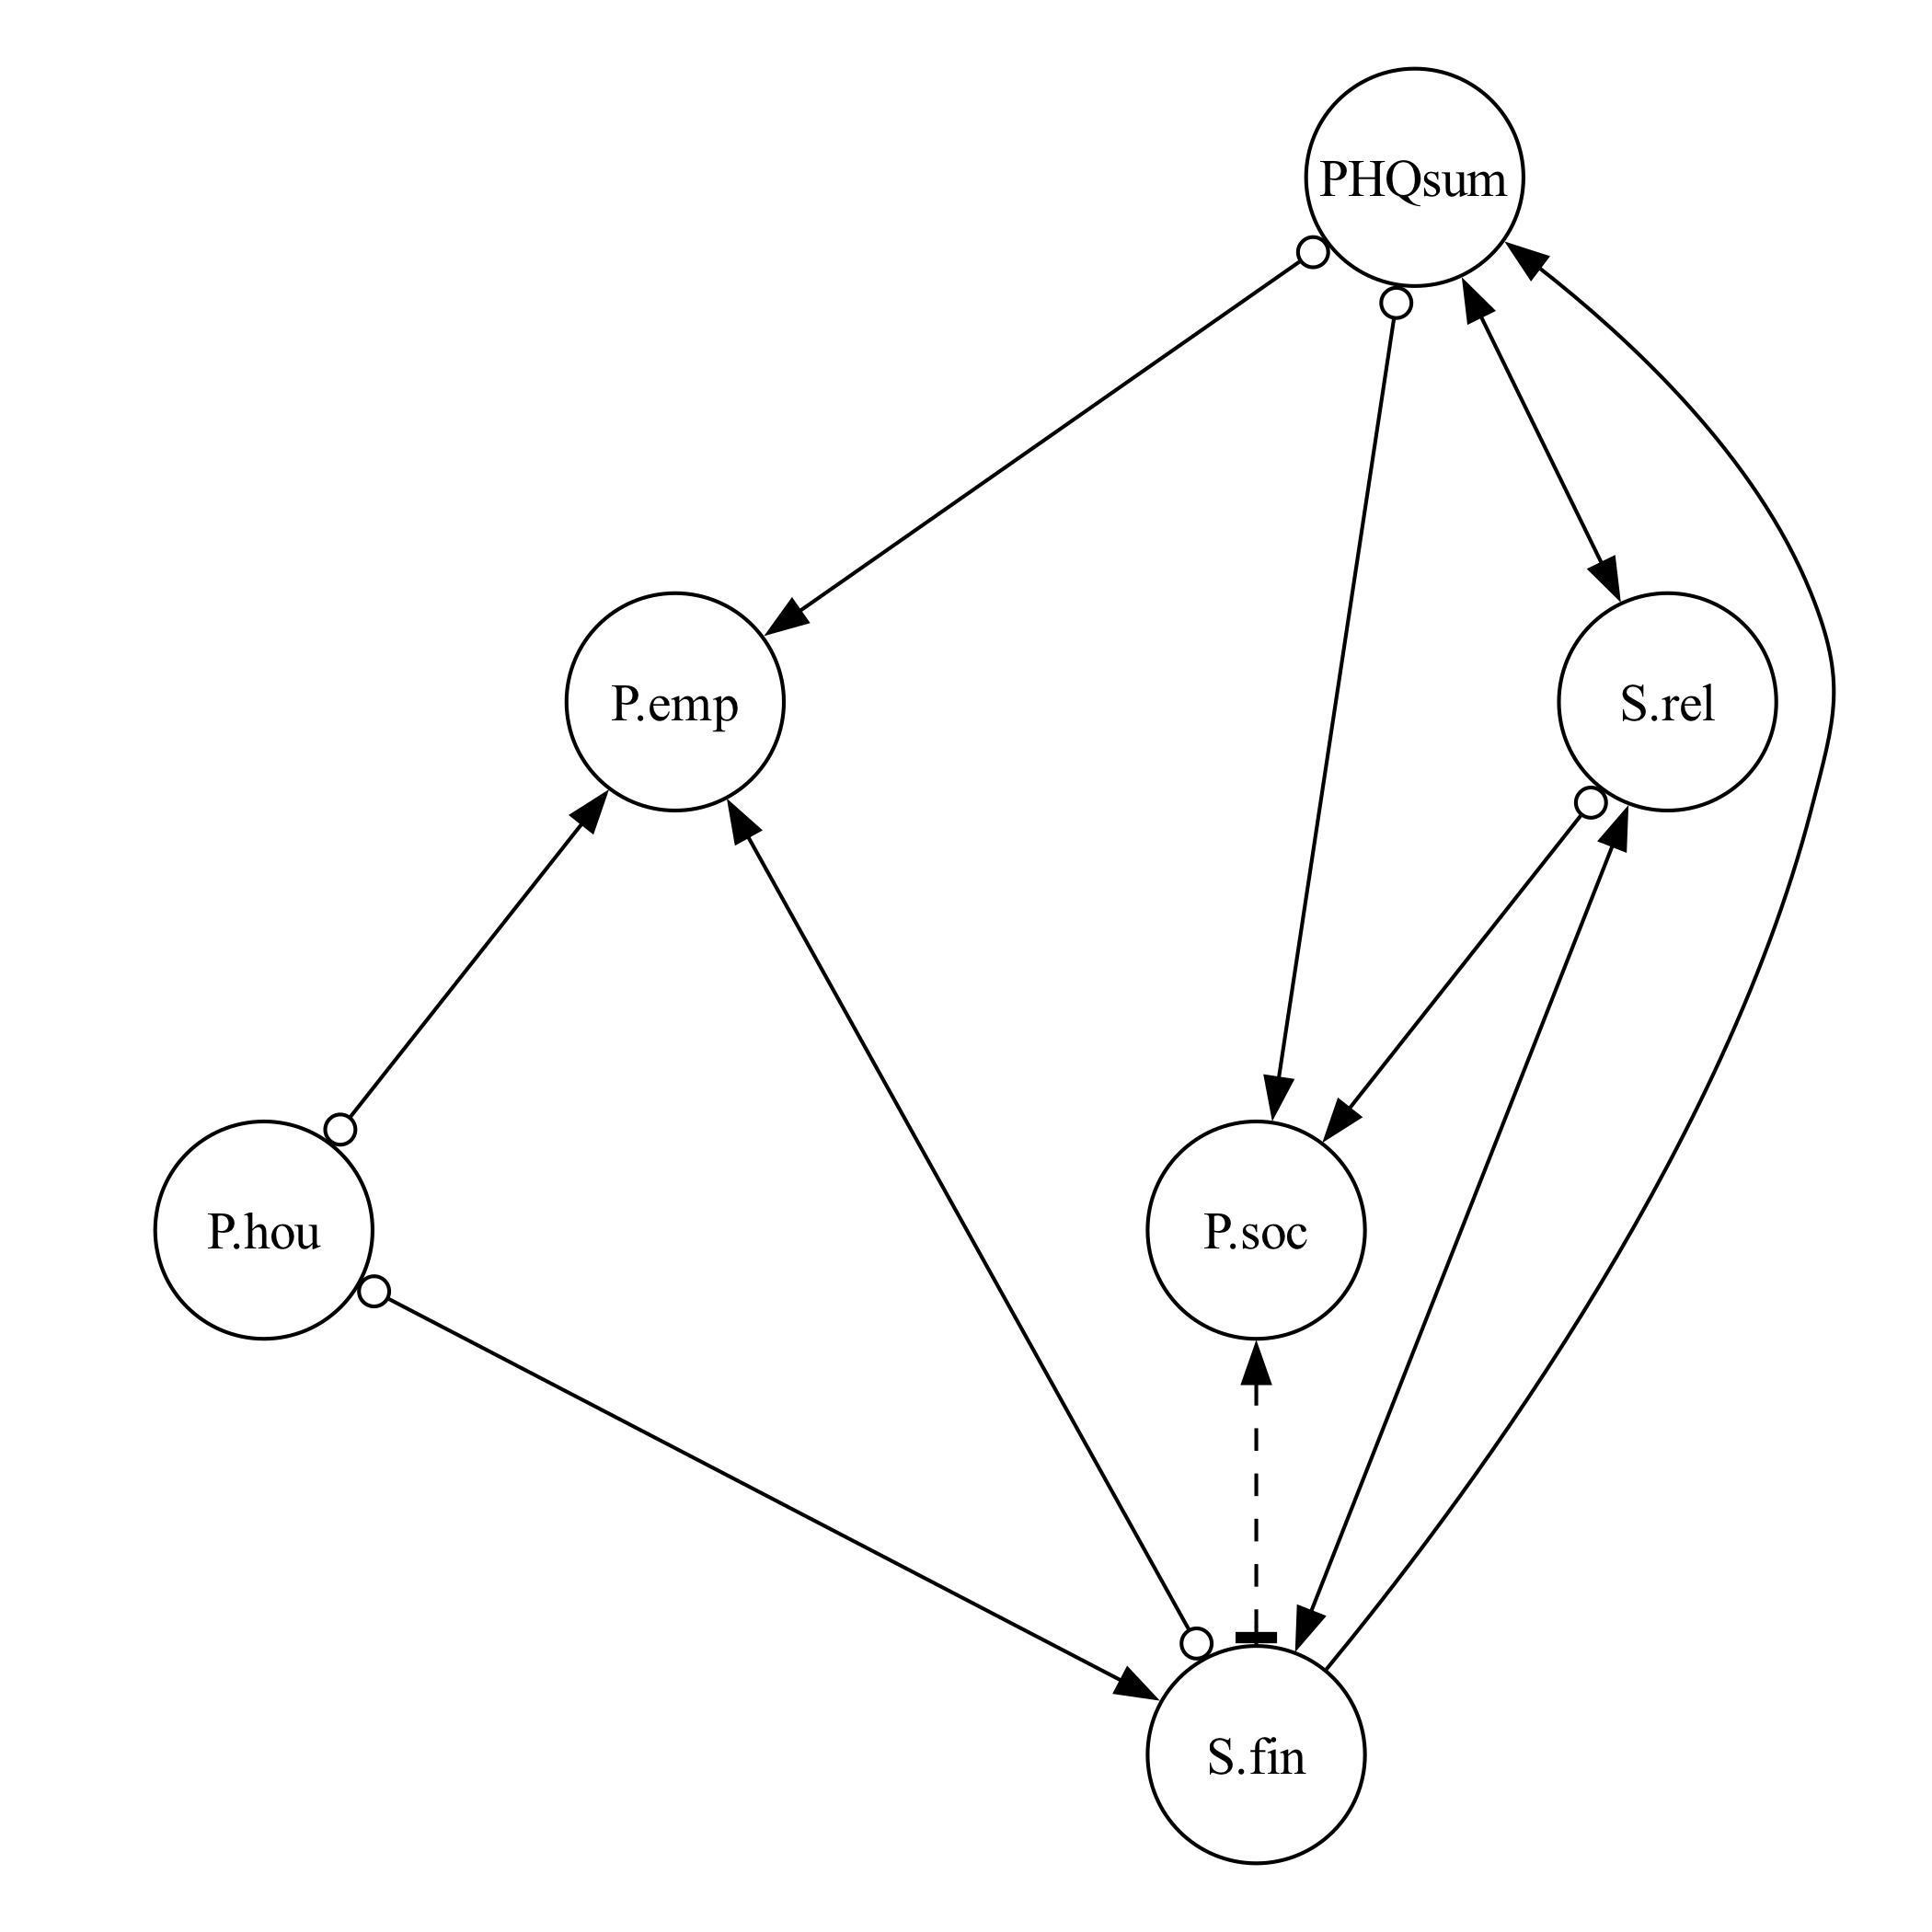
\includegraphics[width=1\textwidth,height=\textheight]{img/FCI_depsum.png}

}

\subcaption{\label{fig-sum-1}FCI PAG}

\end{minipage}%
%
\begin{minipage}{0.50\linewidth}

\centering{

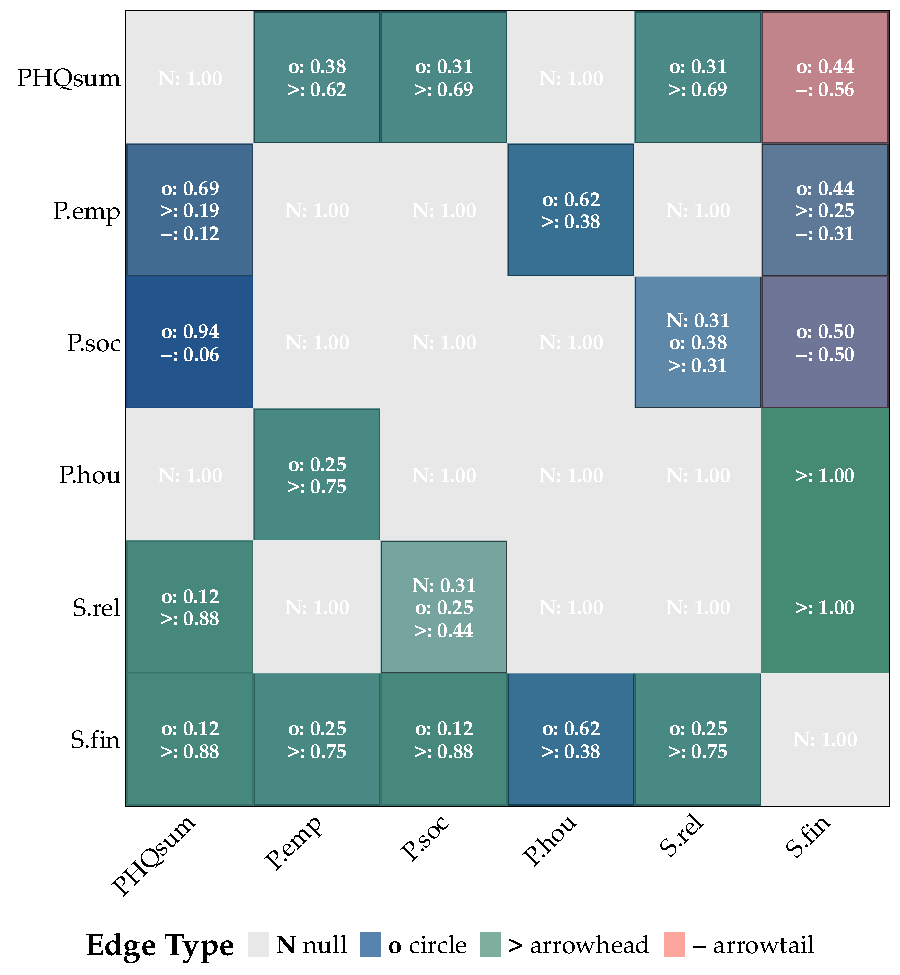
\includegraphics[width=1\textwidth,height=\textheight]{img/depsum_mat_fci.pdf}

}

\subcaption{\label{fig-sum-2}Proportion matrix}

\end{minipage}%

\caption{\label{fig-sum}Causal relationships between five precariousness
factors and depression sum score (\emph{PHQsum}), as estimated using the
FCI algorithm across bootstrapped samples. \textbf{(a)} Aggregated
causal graph showing the most frequent edge types across bootstraps.
Dashed edges indicate ties, with a bold horizontal bar marking where the
tie occurs. \textbf{(b)} Proportion matrix summarizing edge types across
all bootstraps: each matrix cell \([i, j]\) indicates how often a given
edge from variable \(i\) to variable \(j\) exhibited a particular edge
mark (e.g., arrowhead, tail, or circle) adjacent to \(j\). Green
indicates arrowheads, coral arrowtails, blue circle marks, and gray
absence of an edge. Colors are blended and shaded by frequency, with
dominant symbols appearing more opaque. For example,
matrix{[}\(\mathit{S.fin}\), \(\mathit{PHQsum}\){]} shows a green
arrowhead (\(>\)) and matrix{[}\(\mathit{PHQsum}\),
\(\mathit{S.fin}\){]} shows a coral arrowtail (\textemdash), together
indicating that \(\mathit{S.fin} \rightarrow \mathit{PHQsum}\) in the
majority of bootstrapped graphs.}

\end{figure}%

\subsubsection{Individual depression
symptom}\label{individual-depression-symptom}

Moving from the sum score representation to the disaggregated
symptom-level graph provides a more granular perspective on the causal
relationships between precariousness factors and depression symptoms.
Unlike the sum score graph, which aggregates all symptoms into a single
measure, the symptom-level graph in Figure~\ref{fig-sym} reveals the
heterogeneity in how specific symptoms (\emph{con} (concentration),
\emph{slp} (sleep), \emph{ene} (energy), \emph{app} (appetite),
\emph{mot} (motor), \emph{sui} (suicidal), \emph{anh} (anhedonia),
\emph{glt} (guilt), and \emph{dep} (depressed mood)) are influenced by,
and in turn influence, different forms of precariousness.

Figure~\ref{fig-sym-1} reveals a strong interdependence among symptoms
and suggests much presence of latent confounders, as indicated by
numerous bidirectional edges. In Figure~\ref{fig-sym-2}, the proportion
matrix indicates that arrowheads are the most frequently inferred edge
type. However, circle endpoints are particularly common for \emph{anh},
\emph{slp}, \emph{ene}, and \emph{sui}, reflecting uncertainty in the
causal direction among these symptoms. Notably, the only arrowtail
connection appears between \emph{dep} and \emph{anh}, suggesting that
anhedonia is a potential cause of depressed mood.

Looking at the symptom-precariousness connections, one of the key
patterns is that ties are most frequently found in the relationships
between individual symptoms and precariousness factors. This suggests
that these causal links may be less stable across different conditions.
Closer examination reveals that most ties arise due to discrepancies
between the Gaussian CI test and the RCoT test---with Gaussian CI
favoring arrowheads and RCoT more often predicting the absence of an
edge.

Despite these differences, some consistent patterns emerge across both
CI tests, particularly in the case of \emph{S.fin}, which appears to be
connected to nearly all other variables---though many of these
connections are marked by ties, reflecting uncertainty in
directionality. One exception is the stronger evidence suggesting that
\emph{S.fin} may cause changes in \emph{app}, while its relationships
with other symptoms, such as \emph{ene}, \emph{mot}, and \emph{dep},
remain ambiguous. Similarly, \emph{P.soc} exhibits numerous connections
with depressive symptoms, with most edges pointing toward \emph{P.soc}
rather than outward from it. This suggests that depressive symptoms,
particularly \emph{dep} and \emph{glt}, may contribute to worsening
social precariousness rather than the other way around. Additionally,
\emph{anh} also shows signs of a potential causal influence on
\emph{P.soc}, reinforcing the idea that social precariousness is more
often a consequence rather than a driver of depressive symptoms.

Other precariousness factors exhibit more uncertainty but still notable
relationships. \emph{S.rel} is connected to \emph{slp}, \emph{glt}, and
\emph{app}, though directionality remains unclear in many cases.
\emph{P.emp} also connects to symptoms like \emph{slp}, \emph{mot}, and
\emph{con}, but, like \emph{S.rel}, these relationships exhibit a 50/50
split in directionality, reflecting uncertainty in the inferred causal
paths. In line with the aggregated graph in Figure~\ref{fig-sum},
\emph{P.hou} does not appear to have any direct relationship with
depression symptoms but consistently shows associations with
\emph{P.emp} and \emph{S.fin}. The causal relationships among
precariousness factors remain largely unchanged from the aggregated
analysis, with \emph{S.fin} exhibiting the strongest tendency to
influence other precariousness factors.

Among depressive symptoms, \emph{dep}, \emph{glt}, and \emph{slp} appear
to be the most connected to precariousness factors, while \emph{P.soc}
has the most connections with symptoms, predominantly as a recipient
rather than a driver of influence. Within the symptom network,
\emph{slp}, \emph{sui}, and \emph{anh} emerge as causally influential
symptoms, as they exhibit more outgoing arrows compared to other
symptoms. On the other hand, \emph{con}, \emph{mot}, \emph{dep}, and
\emph{glt}, despite having high connectivity, predominantly receive
incoming arrows, indicating they are more likely effects rather than
causes. Considering both symptom-precariousness connections and
symptom-level dynamics, \emph{slp} emerges as a central symptom, given
its strong ties to precariousness factors and its influential role
within the symptom network. \emph{P.soc} appears to function as a bridge
between the depression and precariousness subsystems, as depressive
symptoms appear to feed back into social precariousness, reinforcing a
self-sustaining dynamic between depression and precarious conditions.

Finally, the results from CCI are largely consistent with those from
FCI, but with some key differences. CCI tends to favor arrowheads more
frequently, resulting in a greater number of bidirectional edges, which
suggests a higher involvement of latent confounders. Additionally, CCI
exhibits more tie situations, though, similar to FCI, most ties occur
between absence and arrowhead edges, reflecting the discrepancy between
the Gaussian CI test and RCoT---where the Gaussian test favors
arrowheads, while RCoT more often suggests the absence of an edge. For a
detailed visualization of the CCI-derived graph and proportion matrix,
see Figure~\ref{fig-sym-cci}.

\begin{figure}

\begin{minipage}{\linewidth}

\centering{

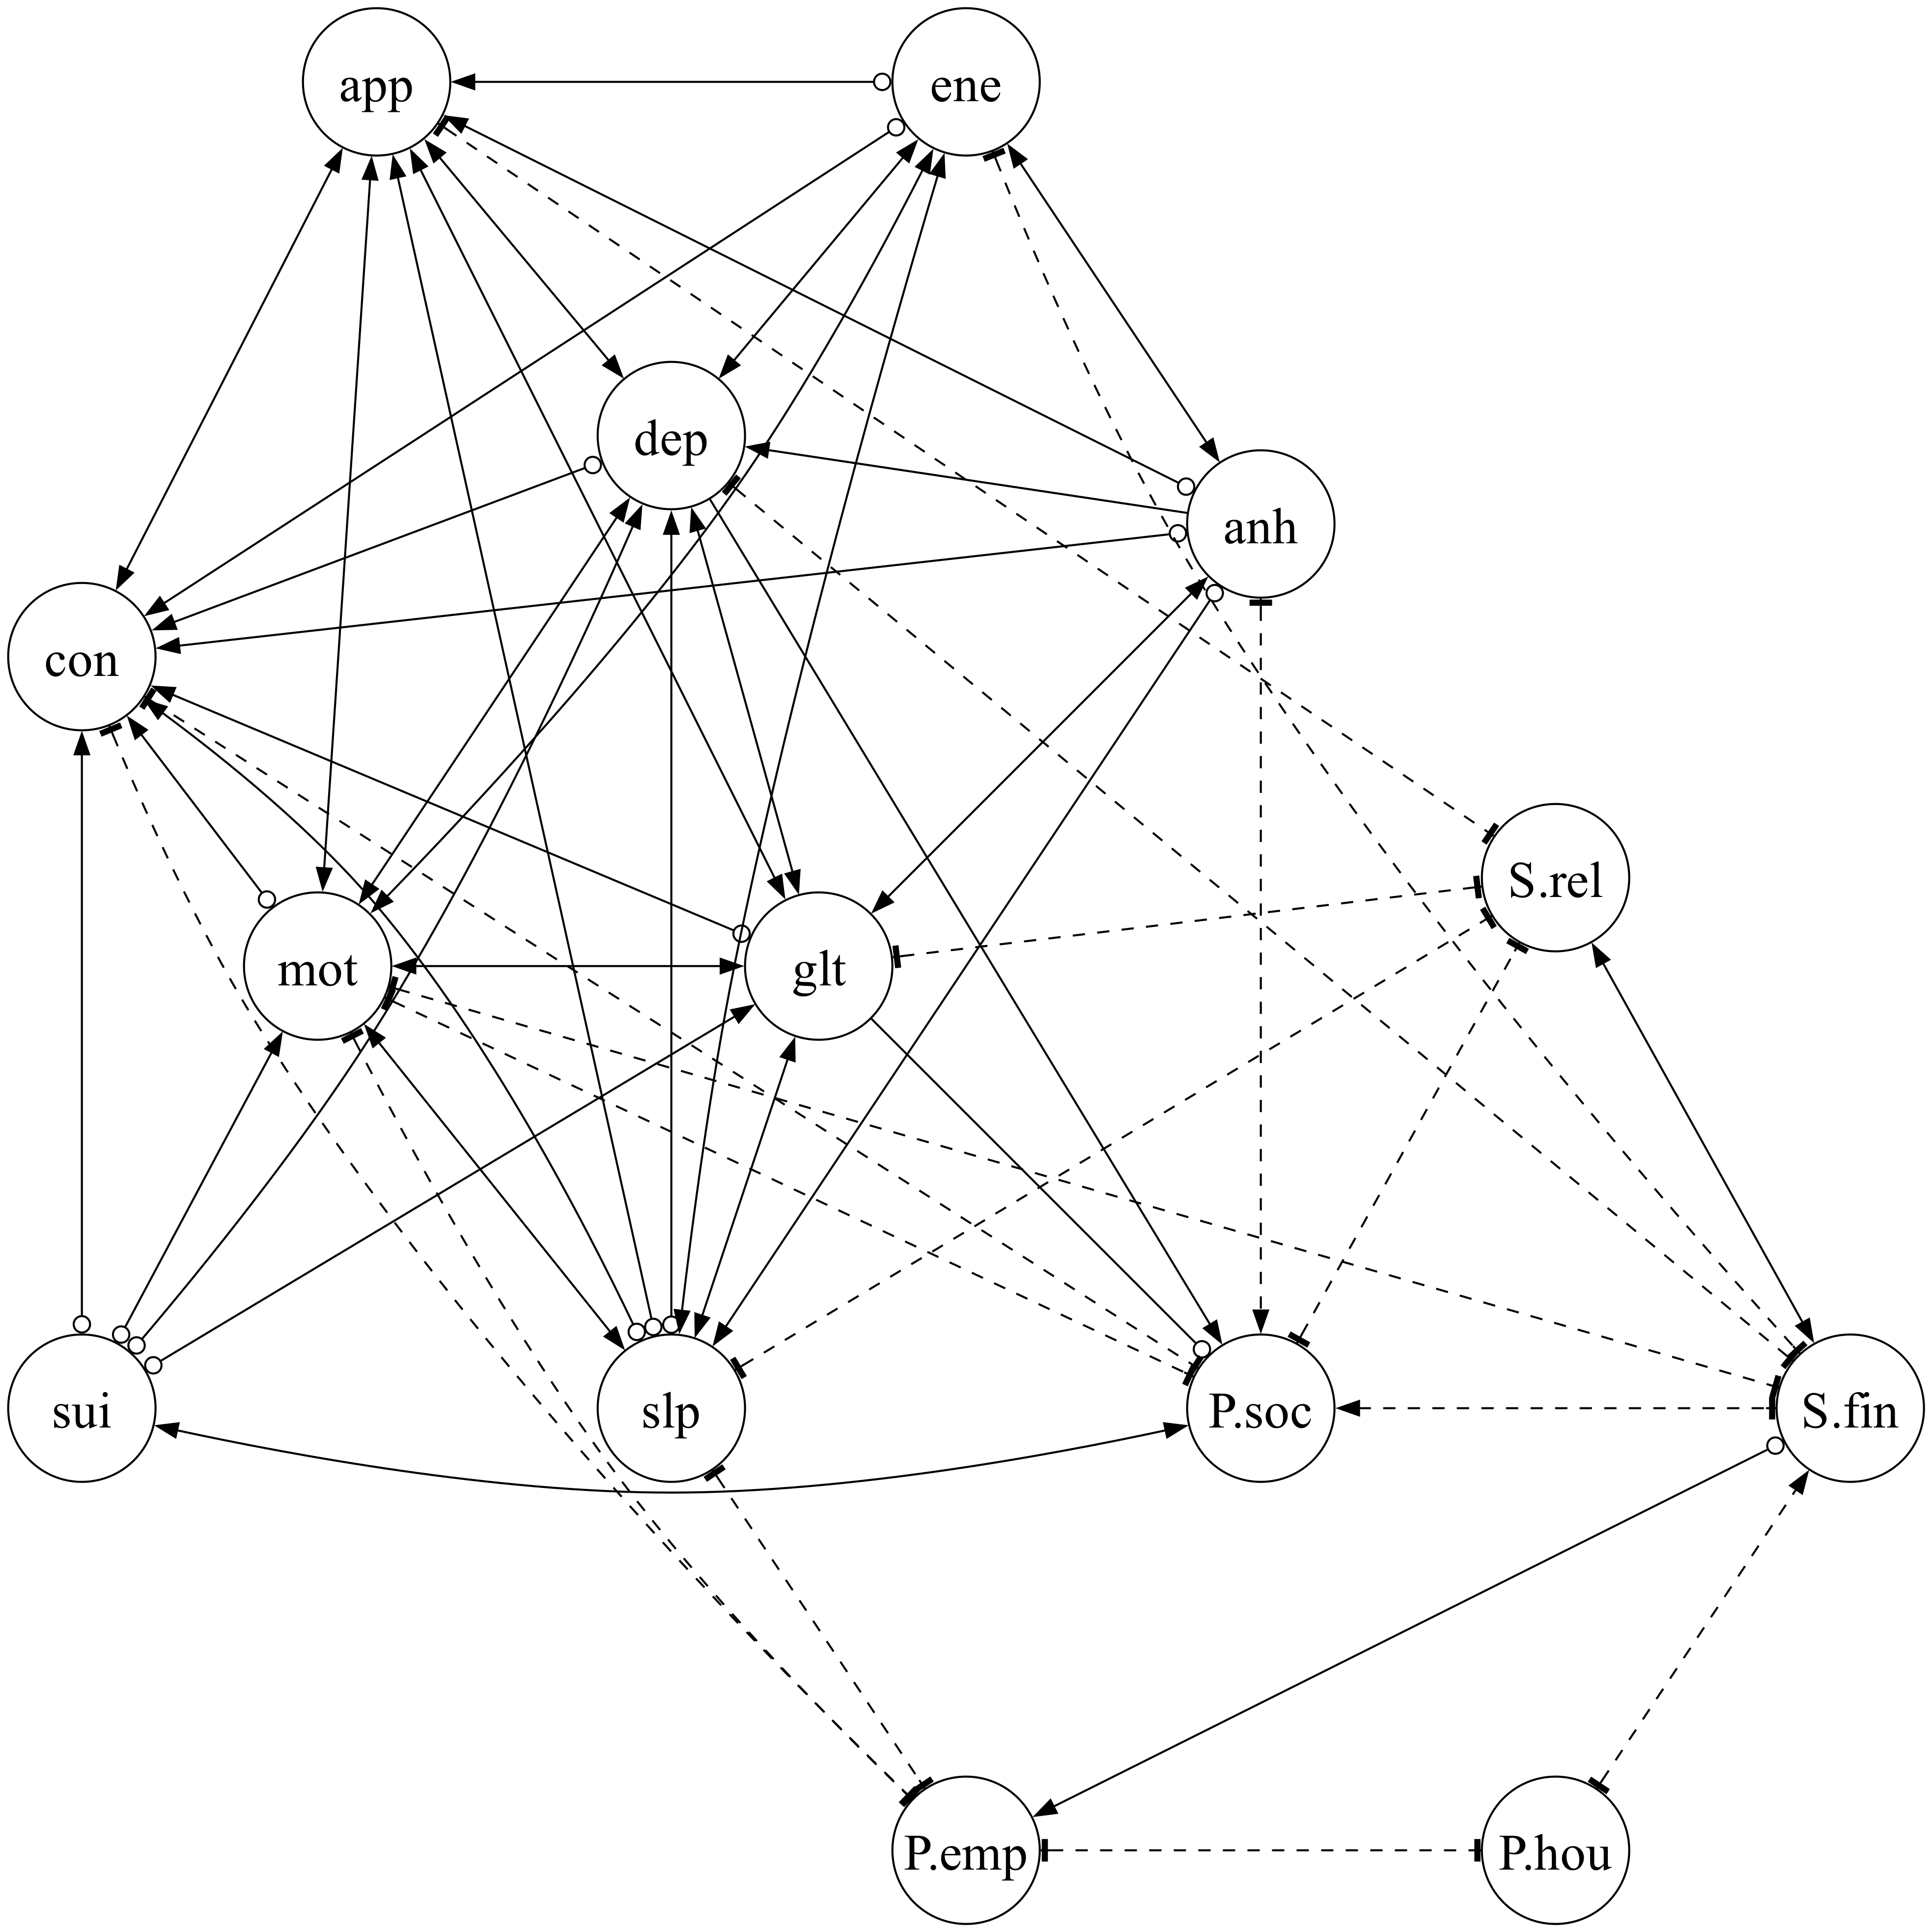
\includegraphics[width=0.7\textwidth,height=\textheight]{img/symptom_graph_FCI.png}

}

\subcaption{\label{fig-sym-1}FCI PAG}

\end{minipage}%
\newline
\begin{minipage}{\linewidth}

\centering{

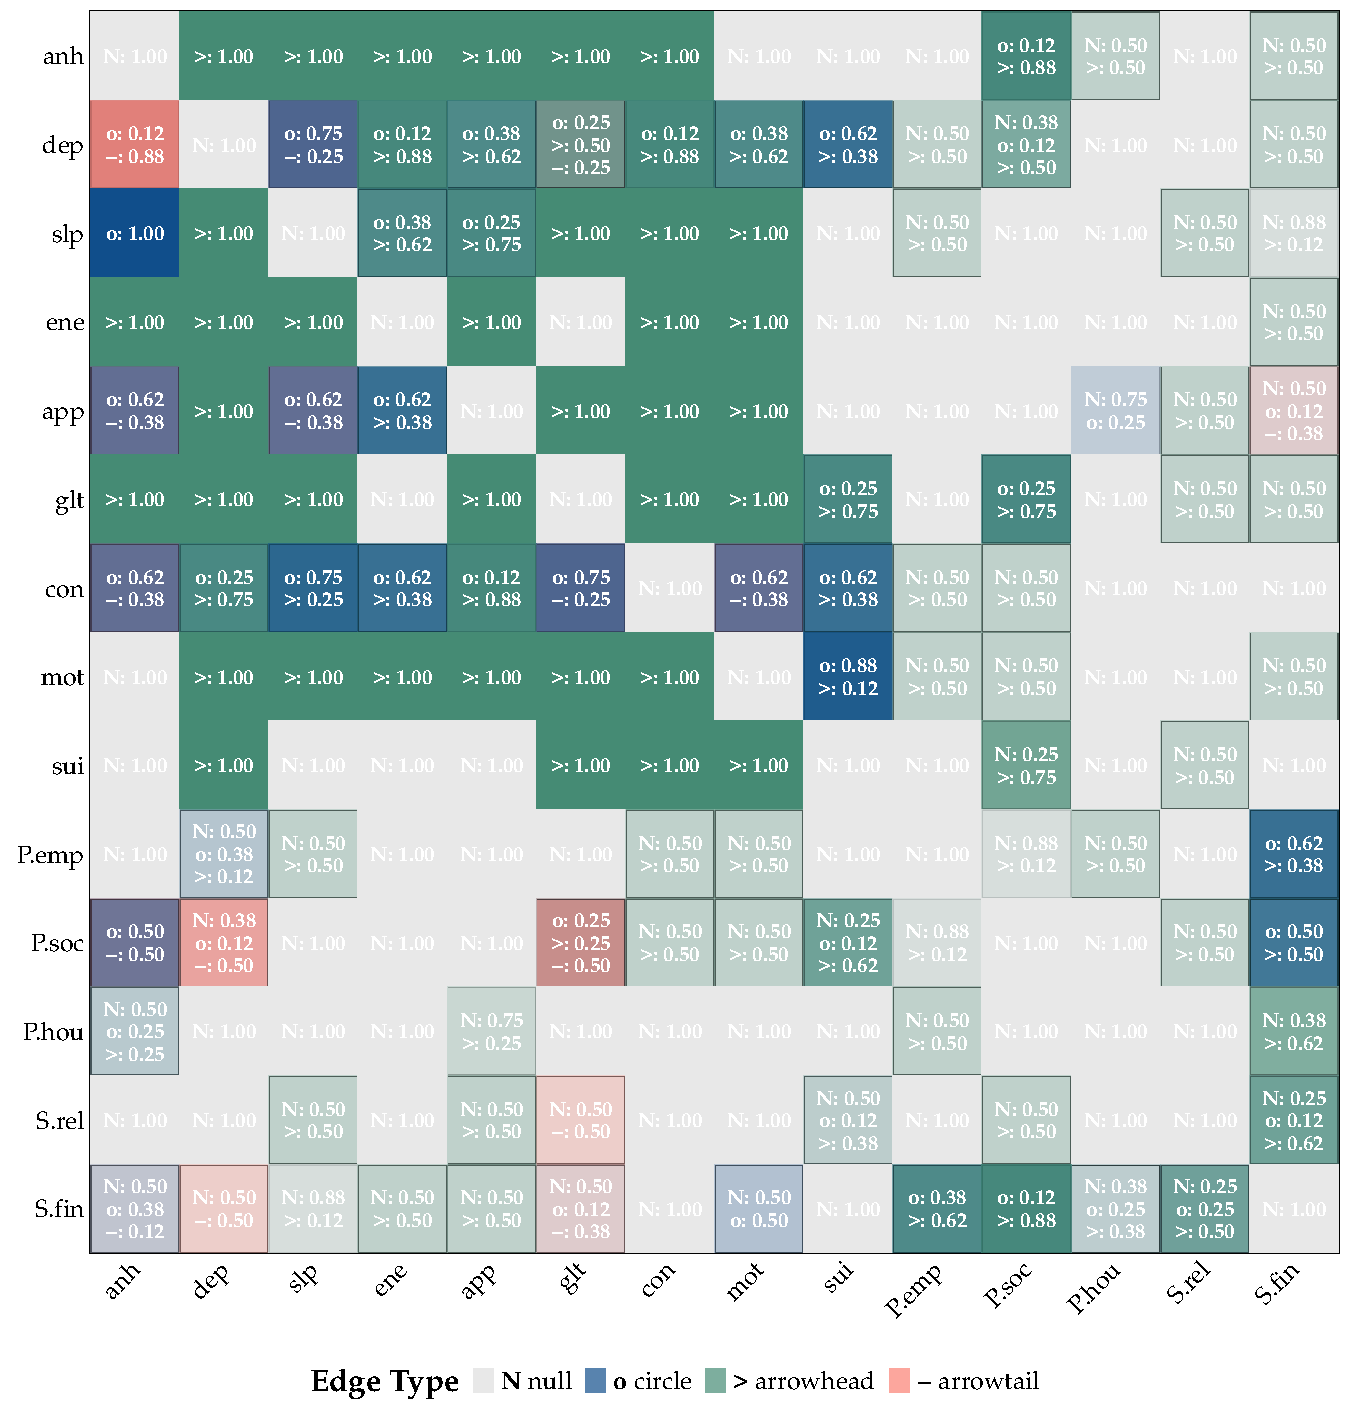
\includegraphics[width=0.7\textwidth,height=\textheight]{img/symptom_mat_fci.pdf}

}

\subcaption{\label{fig-sym-2}Proportion matrix}

\end{minipage}%

\caption{\label{fig-sym}Resulting graph of precariousness factors and
individual depression symptoms using FCI and proportion of edge endpoint
types.}

\end{figure}%

\subsubsection{Precariousness as sum
score}\label{precariousness-as-sum-score}

Lastly, we examine the relationships between individual symptoms and
overall precariousness, an aggregated measure represented by the sum of
five precariousness factors. This analysis provides a complementary
perspective, capturing broader patterns that may not be evident in the
disaggregated symptom-precariousness analysis. By aggregating
precariousness factors into a single score, this approach may capture
distributed relationships across different precariousness factors that
were previously overlooked in the disaggregated analysis.

Unlike the disaggregated graph in Figure~\ref{fig-sym}, the aggregated
symptom-precariousness graph (Figure~\ref{fig-presum-1}) shows greater
certainty in causal directions, with ties occurring only in edges
involving the overall precariousness factor. This is even more evident
in the proportion matrix (Figure~\ref{fig-presum-2}), where
symptom-to-symptom interactions almost fully converge to a single edge
type. Additionally, all symptom interactions are connected either
through bidirectional edges or a combination of an arrowhead and a
circle, suggesting a strong presence of latent confounders.

Examining the symptom-precariousness connections, we observe a stronger
overall trend of depressive symptoms influencing precariousness, rather
than the other way around. Specifically, \emph{anh}, \emph{dep}, and
\emph{slp} frequently emerge as sources of influence on precariousness,
whereas \emph{app}, \emph{glt}, and \emph{mot} exhibit more uncertainty
in directionality, often resulting in circle endpoints. This pattern
suggests that when precariousness factors are aggregated, the dominant
causal flow is from depressive symptoms to precariousness, rather than
precariousness driving depression. Particularly, \emph{dep} emerges as
the strongest predictor of precariousness, exhibiting the highest
proportion of arrowtails, consistent with findings from the
disaggregated analysis.

Comparing this with the CCI-derived graph (Figure~\ref{fig-presum-cci}),
several key differences stand out. The CCI results reveal that most
symptoms are interconnected through bidirectional edges, suggesting a
strong presence of latent confounders. However, \emph{dep} appears to be
a distinct exception, as it is predominantly caused by nearly all other
symptoms, with one exception \emph{sui}, which does not contribute to
\emph{dep}. Similarly, \emph{con} is influenced by multiple symptoms,
albeit with weaker support compared to \emph{dep}. Most interestingly,
the CCI results highlight a distinct feedback loop between \emph{dep}
and overall precariousness, represented by a tail-tail edge
(\textemdash ). This suggests a possible reinforcing cycle between
depression and overall precariousness, where depression not only arises
from precarious conditions but also contributes to their persistence,
creating a self-sustaining dynamic.

Across multiple levels of analysis, our results point to a consistent
and directional link between precariousness and depression. Financial
stress (\emph{S.fin}) emerges as a particularly robust and modifiable
upstream driver: in both aggregated and disaggregated models, it shows
strong and stable causal influence on depressive symptoms. By contrast,
other forms of precariousness---particularly social precarity---more
often appear as outcomes rather than antecedents of depression,
frequently receiving rather than sending causal arrows. Among symptoms,
\emph{dep} and \emph{slp} stand out for their centrality and connections
to precariousness factors, with \emph{dep} also implicated in potential
feedback loops with social precarity (\emph{P.soc}). These findings
motivate the use of a simplified three-node model in the
simulation---capturing depression, financial stress, and social
precarity---as it preserves the key dynamic motifs observed in the
causal graphs while enabling tractable exploration of system-level
responses to stress-reducing interventions.

\begin{figure}

\begin{minipage}{\linewidth}

\centering{

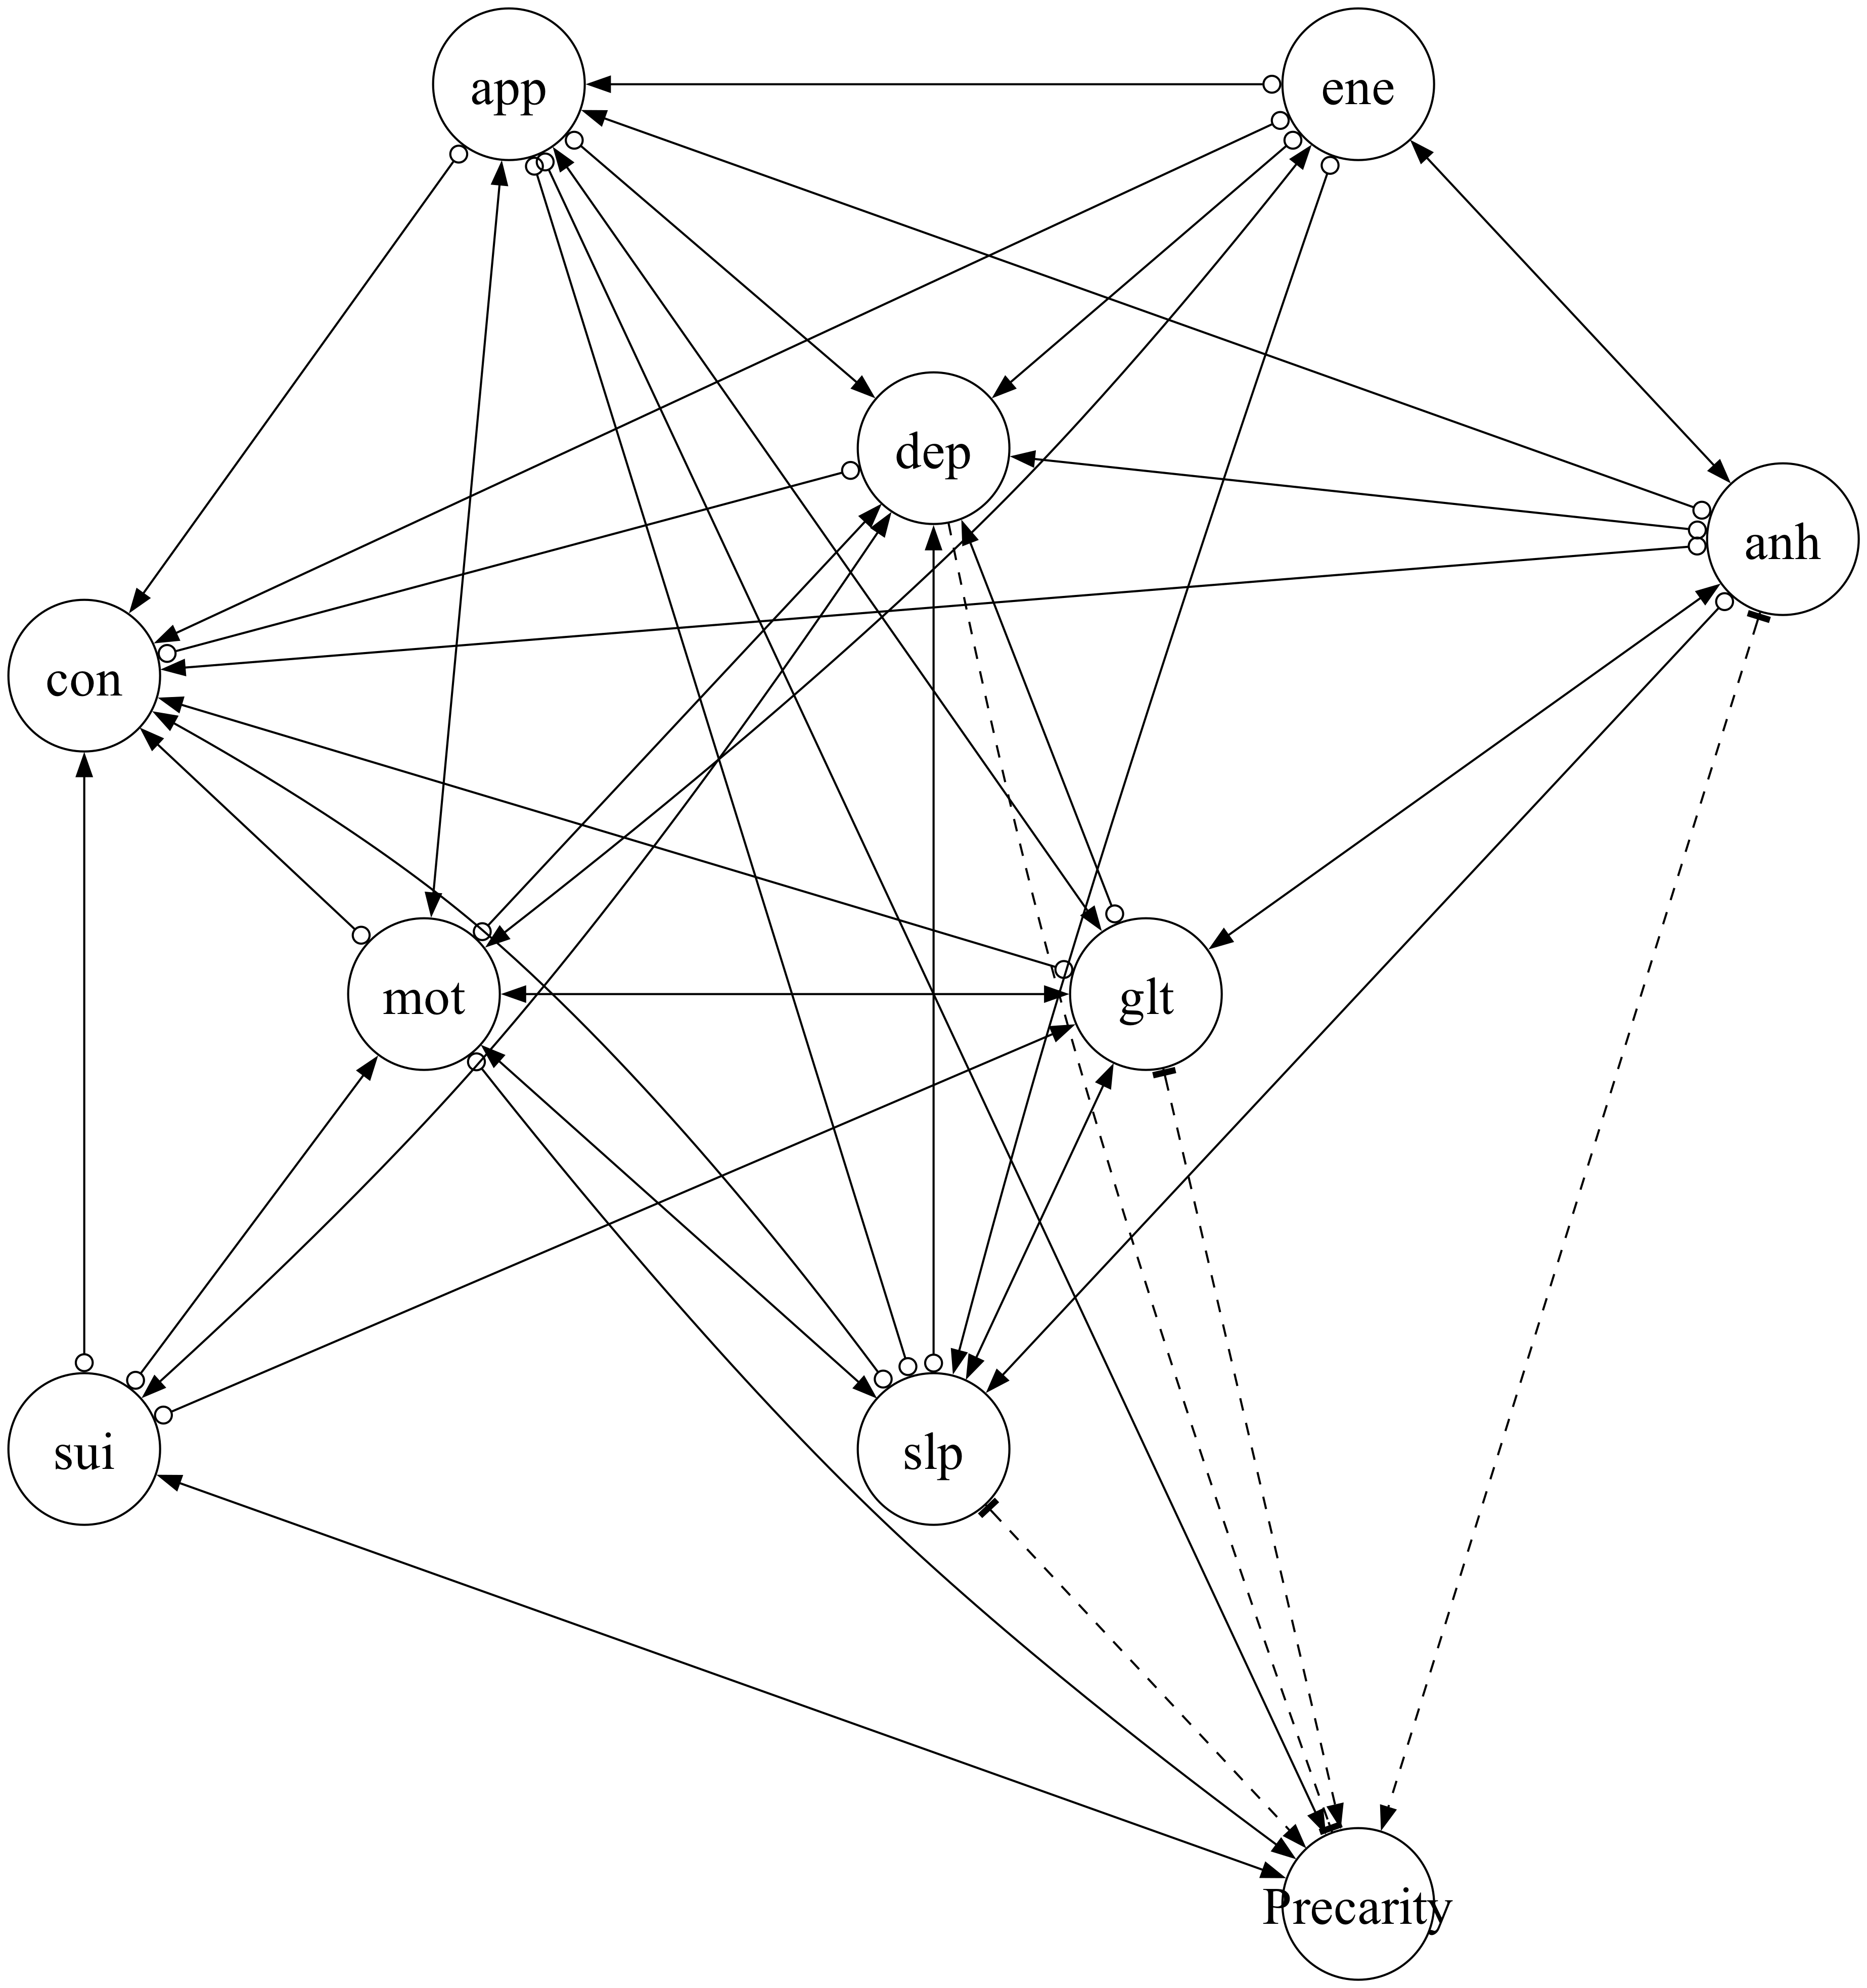
\includegraphics[width=0.6\textwidth,height=\textheight]{img/presum_graph_FCI.png}

}

\subcaption{\label{fig-presum-1}FCI PAG}

\end{minipage}%
\newline
\begin{minipage}{\linewidth}

\centering{

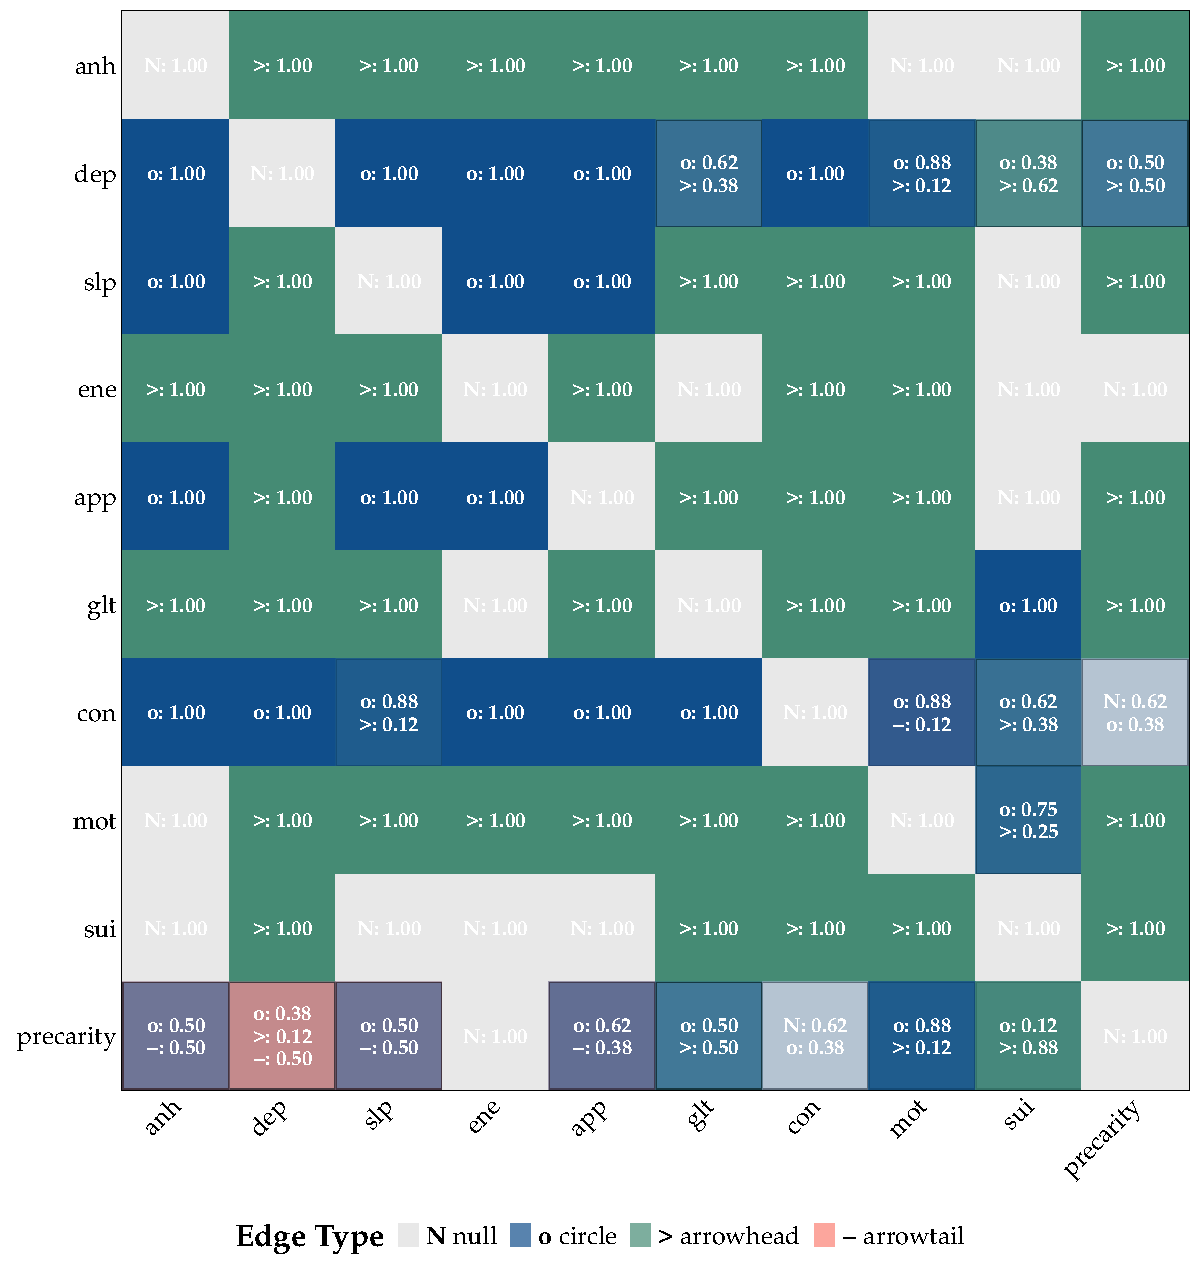
\includegraphics[width=0.6\textwidth,height=\textheight]{img/presum_mat_fci.pdf}

}

\subcaption{\label{fig-presum-2}Proportion matrix}

\end{minipage}%

\caption{\label{fig-presum}Resulting graph of precariousness sum score
and individual depression symptoms using FCI and proportion of edge
endpoint types. As before, dashed edges denote ties, with specific ties
marked by bold horizontal bars.}

\end{figure}%

\subsection{Simulating the Dynamics Between Precariousness and
Depression Under
Intervention}\label{simulating-the-dynamics-between-precariousness-and-depression-under-intervention}

To assess how internal structure influences the system's responsiveness
to external support, we simulate a set of linear models that are
consistent with the data but vary in the assumed strength of influence
from precariousness to depression (\(\alpha_{DP}\)). For each model, we
generate a virtual population of 1,000 individuals and simulate an
external intervention that reduces each individual's financial stress
(\(S\)) proportionally toward the minimum observed value in the dataset.
While individuals begin with different baseline stress levels, the
intervention applies a shared proportional reduction across the
population. This intervention defines the external input, while
variation in \(\alpha_{DP}\) reflects different assumptions about
internal feedback from precariousness to depression. We examine system
behavior in two complementary ways: (1) by analyzing average levels of
depression and precariousness at selected time points following
intervention onset, and (2) by simulating full temporal trajectories
under sustained intervention followed by recovery, using two
representative cases at the extremes of the \(\alpha_{DP}\) range.

Figure~\ref{fig-intervention} summarizes how variation in
\(\alpha_{DP}\) shapes system-level responses to external support. In
Panel A, during the early phase of intervention, depression and
precariousness exhibit contrasting patterns. Depression declines more
rapidly in scenarios with lower \(\alpha_{DP}\), where its dynamics are
driven more directly by the external stressor \(S\). As \(\alpha_{DP}\)
increases, \(D\) becomes more dependent on precariousness (\(P\)), which
itself adjusts more slowly---delaying the depressive response.
Precariousness, by contrast, shows slightly faster early reductions in
scenarios with higher \(\alpha_{DP}\). This reflects a shift in
influence: as \(\alpha_{DP}\) increases, \(P\) becomes more directly
responsive to \(S\) (via increasing \(\alpha_{PS}\)) and less influenced
by \(D\), allowing it to adjust more promptly to changes in the
stressor.

Despite these short-term differences, all scenarios ultimately converge
to similar steady-state levels under sustained intervention. AS the
systm approaches convergence, some variation remains, particularly in
\(P\), where gradients between models are still visible. This
convergence highlights that the key distinctions lie not in whether
intervention is effective, but in how quickly and through which pathways
change unfolds.

Panel B shows full time trajectories for two representative cases: one
with minimal internal feedback (\(\alpha_{DP} = 0\)) and one at the
upper admissible limit (\(\alpha_{DP} = 0.65\)). In both, there is a
temporary intervention period. When \(\alpha_{DP} = 0\), depression
responds rapidly to the reduction in stress and rebounds shortly after
support is withdrawn. In contrast, when \(\alpha_{DP}\) is high, \(D\)
responds more gradually and recovers more slowly---reflecting its
increased dependence on the slower-changing \(P\). Precariousness
declines in both scenarios during intervention and returns to baseline
afterward, but with a slightly sharper drop in the higher
\(\alpha_{DP}\) condition. This occurs because \(P\) becomes more
directly responsive to \(S\), as consistency with the data requires
\(\alpha_{PS}\) to increase with \(\alpha_{DP}\) (see
Figure~\ref{fig-tradeoff}). These parameter shifts reflect trade-offs
needed to preserve the empirical covariances, with further details
provided in Appendix Section~\ref{sec-analcalibration}.

These asymmetries further highlight how internal structure---not just
external inputs---shapes the system's trajectory. Specifically, changes
in coupling parameters reconfigure how stress reduction propagates
through the system, altering the speed and pathway of response even when
long-run outcomes remain unchanged.

\newgeometry{top=20mm, bottom=20mm, left=40mm, right=40mm}

\begin{figure}

\centering{

\includegraphics[width=0.8\textwidth,height=\textheight]{img/intervention_linear.pdf}

}

\caption{\label{fig-intervention}System response to external
intervention across variations in internal structure.
\emph{\textbf{Panel A}: Mean levels of depression (\(D\)) and
precariousness (\(P\)) at time steps 100, 300, and 500, across varying
values of \(\alpha_{DP}\) and intervention strengths. The x-axis
represents the strength of external support, operationalized as the
proportional reduction of financial stress (\(S\)) toward its minimum
observed value. Each line corresponds to a different model defined by a
specific \(\alpha_{DP}\) value, color-coded from low (purple) to high
(yellow). Models with lower \(\alpha_{DP}\) exhibit faster early
reductions in \(D\), while higher \(\alpha_{DP}\) leads to more
immediate declines in \(P\). \textbf{Panel B}: Full time trajectories
for two models---one with no coupling (\(\alpha_{DP} = 0\)) and one with
strong coupling (\(\alpha_{DP} = 0.65\))---illustrating system response
and recovery following intervention onset (step 300) and withdrawal
(step 1500). Depression responds more gradually and persistently in the
high \(\alpha_{DP}\) model, whereas precariousness adjusts more
quickly.}}

\end{figure}%

\restoregeometry

\section{Discussion}\label{discussion}

This study combined constraint-based causal discovery and dynamical
modeling to investigate how depression and socioeconomic precariousness
interact and how their internal structure modulates responsiveness to
intervention. Consistent with prior work linking financial strain to
psychological distress (Ezzy, 1993; Lund et al., 2010), our analysis
identified financial stress as a key upstream driver of depression in
both aggregated and disaggregated models. This supports longstanding
hypotheses that economic stressors can act as modifiable entry points
into broader cycles of psychosocial risk.

At the symptom level, our analysis aligns with established theories of
psychopathology but provides a more fine-grained map of potential causal
relationships, generating concrete, testable hypotheses. It also points
to possible limitations of prevailing models, as some observed
symptom--symptom links may be shaped by shared confounders rather than
direct causal influence. This suggests that, in some contexts, broader
mechanisms or clusters of symptoms may provide more effective units of
analysis and intervention than individual symptoms alone. Within this
framework, sleep disturbance emerged as a potentially initiating
symptom, with directed connections to both symptom-level and
precariousness variables---mirroring longitudinal findings that identify
sleep disruption as an early warning signal for depressive episodes and
social withdrawal (Alvaro et al., 2013; Zawadzki et al., 2013).
Depressed mood, another core symptom, occupied a central position in the
network. Not only was it influenced by upstream symptoms like anhedonia
and guilt, but it also showed directional influence on social
precariousness---suggesting that internal psychological states may
actively shape external vulnerability. The CCI algorithm further
identified a potential feedback loop between depressed mood and overall
precariousness, resonating with social drift theories in depression,
which posit that declining mental health can lead to social exclusion,
job instability, and housing insecurity, reinforcing depressive cycles
(Boschloo et al., 2015; Compton \& Shim, 2015).

In contrast, social precariousness itself appeared more often as an
effect than a cause, receiving arrows from symptoms like depressed mood
and guilt but rarely sending them. This asymmetry supports prior
observations that indicators of social vulnerability often reflect
downstream consequences of poor mental health, though the relationships
are likely bidirectional over time (Lund et al., 2010). Although our
findings are based on Amsterdam-specific data, they align with research
in other high-income urban settings, where structural inequalities such
as poverty, unemployment, and housing insecurity consistently predict
poor psychological outcomes (Fryers et al., 2003; Weich \& Lewis, 1998).
While local contexts may alter specific pathways, these parallels
suggest that similar mechanisms could operate elsewhere, though
replication in other populations is needed to assess robustness.

Taken together, these findings yield actionable insights for mental
health intervention. Symptoms like sleep disturbance, which demonstrate
early and broad influence across both symptom and precariousness
networks, may serve as effective targets for prevention---potentially
halting the progression into more entrenched depressive states or
worsening precariousness. Similarly, targeting symptoms such as
depressed mood, which appear embedded in potential feedback loops
linking psychological and social domains, may offer strategic leverage
for breaking mutually reinforcing cycles of mental decline and social
isolation. Importantly, interventions targeting such nodes may have
ripple effects across domains. For instance, evidence suggests that
treating core depressive symptoms can improve social functioning,
employment engagement, and housing stability---particularly when
combined with social or financial supports (Lund et al., 2018; McDaid et
al., 2019). These dual benefits underscore the value of integrated,
cross-domain strategies that simultaneously address internal symptoms
and external stressors.

Our results also highlight why single-point interventions may fail to
produce lasting change. The broader causal structure reveals multiple
interlocking feedback loops spanning both psychological symptoms and
structural risk factors, which may re-amplify vulnerability even after
temporary relief. Supporting this, recent simulation work by Park, Li,
et al. (2025) shows that feedback loops, even when modest in strength,
can substantially diminish the long-term impact of isolated
interventions unless multiple reinforcing links are simultaneously
disrupted. Our own simulations support this view: while all models
converged to similar long-term outcomes under sustained support,
differences in internal structure---specifically, the strength of the
link from precariousness to depression---produced systematic variation
in how quickly and through which pathways systems responded to
intervention. Stronger coupling slowed recovery and prolonged
depression, showing that internal architecture can be as important as
external input. This supports growing calls for systems-oriented mental
health perspectives (Borsboom, 2017). Rather than assuming uniform
responses, more durable outcomes may require (1) targeting early-acting
symptoms, (2) sustaining support where recovery is slow, and (3)
combining structural and psychological interventions. Tailoring
strategies to match the system's architecture can improve effectiveness,
particularly in populations with layered vulnerabilities. In this light,
understanding causal architecture is not merely theoretical---it is
foundational to designing more effective and equitable interventions.

While the FCI and CCI algorithms are designed to recover causal
structure from cross-sectional data---including feedback and latent
confounding---many edge directions in our results remain ambiguous,
particularly in links between individual symptoms and precariousness
factors. These inconsistencies likely reflect limited statistical signal
in high-dimensional settings, where large conditioning sets reduce power
and small effect sizes are harder to detect. Moreover, our findings
showed sensitivity to the choice of conditional independence (CI) test.
The Gaussian CI test, which assumes linearity and Gaussian noise, often
produced denser graphs, likely due to overestimating weak or noisy
linear associations. In contrast, RCoT, a nonparametric alternative,
avoids these assumptions but relies on a Gaussian radial basis function
(RBF) kernel to assess dependence. While flexible in capturing nonlinear
relationships, this kernel is optimized for smooth, continuous variables
and may underperform with discrete or ordinal data. Its similarity
estimates can be unreliable when applied to variables with
discontinuities, potentially leading to missed dependencies. This is
particularly relevant in the HELIUS dataset, where some variables are
ordinal or mixed-type (Howlett, 2001). To address this, future work
should consider adapting kernel-based CI tests to better handle mixed
data structures---for example, by employing hybrid kernels that
explicitly combine continuous and discrete similarity measures. This
could improve the reliability of nonparametric causal discovery in
settings with heterogeneous variable types.

Although the CCI algorithm is explicitly designed to detect cycles,
aside from the connection between precarity and depression in the
aggregate precarity setting, we found little clear evidence of feedback:
most candidate loops appeared only as bidirectional edges, which may
reflect latent confounding or statistical imprecision. This could point
to either an absence of strong feedback at the symptom and the
precariousness factor levels or limitations in the sensitivity of
full-graph discovery approaches applied to densely interconnected
variables. More focused strategies, such as local structure tests or
theory-guided subgraph modeling, may help resolve these ambiguities.
Moreover, our analyses relied solely on observational data from the
Amsterdam population. Some structural uncertainties, particularly those
involving latent confounding or bidirectional influence, may ultimately
require interventional or semi-interventional designs. Extensions such
as LLC (Hyttinen et al., 2012), NODAGS-Flow (Sethuraman et al., 2023),
or Bicycle (Rohbeck et al., 2024), which integrate observational and
interventional data, could be especially valuable where such data are
available.

Finally, the structure of our dynamical model introduces important
limitations. The model focused on a restricted set of variables
(depression, social precariousness, and financial stress). This design
was intentionally simplified to isolate core mechanisms of interest, but
it necessarily omits other relevant domains of precariousness,
additional stressors, and potential unintended consequences of
intervention. In addition, while the linear formulation offered
analytical tractability and transparent calibration, it likely
oversimplifies the true dynamics of depression and socioeconomic
precariousness. A growing body of evidence suggests that psychosocial
systems are fundamentally nonlinear. Empirical and theoretical work
points to phenomena such as threshold effects, where improvements only
occur after a tipping point is crossed (Leemput et al., 2014; Park,
Waldorp, et al., 2025); saturation, where the impact of support
diminishes as basic needs are met (Cramer et al., 2010); and path
dependence, where past adversity shapes sensitivity to future stressors
(Wichers et al., 2016). These behaviors are fundamentally incompatible
with linear dynamics, yet they may be essential for understanding why
some individuals remain trapped in high-risk states while others recover
more easily. Future modeling efforts should therefore incorporate
mechanisms such as saturating input-response functions (e.g., sigmoidal
form) and state-dependent feedback (where coupling strength varies by
system state). Incorporating such features would allow models to capture
not just average effects but also the critical conditions under which
meaningful change becomes possible---clarifying whether some subgroups
require forceful, threshold-crossing interventions, while others may
benefit from sustained, moderate support.

As public health research has long shown, social and psychological
systems do not always respond passively to external inputs; internal
constraints can limit the impact of even well-intentioned policies
(Savigny \& Adam, 2009; Wagenaar \& Burris, 2013). By using causal
discovery and computational modeling, researchers and policymakers can
better identify these structural constraints and tailor interventions
accordingly. More broadly, this study offers a generalizable framework
for investigating complex mental health dynamics. Causal discovery
supports principled hypothesis generation from observational data, while
dynamical modeling enables exploration of how hypothesized structures
behave under external change. Together, these tools move us beyond
static descriptions toward mechanistic insight with direct relevance for
real-world mental health policy and intervention design. Future research
should build on this foundation by developing richer, more nuanced
dynamical models grounded in longitudinal and interventional data.
Incorporating time, multiple domains of precarity, and adaptive feedback
processes would help assess whether the mechanisms proposed manifest in
actual mental health trajectories. Ultimately, we hope this study
encourages further integration of causal structure learning and systems
modeling in efforts to understand and improve mental health outcomes
under conditions of socioeconomic precariousness.

\section{References}\label{references}

\phantomsection\label{refs}
\begin{CSLReferences}{1}{0}
\bibitem[\citeproctext]{ref-alvaro2013systematic}
Alvaro, P. K., Roberts, R. M., \& Harris, J. K. (2013). A systematic
review assessing bidirectionality between sleep disturbances, anxiety,
and depression. \emph{Sleep}, \emph{36}(7), 1059--1068.

\bibitem[\citeproctext]{ref-borsboom2017network}
Borsboom, D. (2017). A network theory of mental disorders. \emph{World
Psychiatry}, \emph{16}(1), 5--13.

\bibitem[\citeproctext]{ref-boschloo2015network}
Boschloo, L., Van Borkulo, C. D., Rhemtulla, M., Keyes, K. M., Borsboom,
D., \& Schoevers, R. A. (2015). The network structure of symptoms of the
diagnostic and statistical manual of mental disorders. \emph{PloS One},
\emph{10}(9), e0137621.

\bibitem[\citeproctext]{ref-butterworth2012role}
Butterworth, P., Olesen, S. C., \& Leach, L. S. (2012). The role of
hardship in the association between socio-economic position and
depression. \emph{Australian \& New Zealand Journal of Psychiatry},
\emph{46}(4), 364--373.

\bibitem[\citeproctext]{ref-compton2015social}
Compton, M. T., \& Shim, R. S. (2015). The social determinants of mental
health. \emph{Focus}, \emph{13}(4), 419--425.

\bibitem[\citeproctext]{ref-cramer2010comorbidity}
Cramer, A. O., Waldorp, L. J., Van Der Maas, H. L., \& Borsboom, D.
(2010). Comorbidity: A network perspective. \emph{Behavioral and Brain
Sciences}, \emph{33}(2-3), 137--150.

\bibitem[\citeproctext]{ref-deb2002fast}
Deb, K., Pratap, A., Agarwal, S., \& Meyarivan, T. (2002). A fast and
elitist multiobjective genetic algorithm: NSGA-II. \emph{IEEE
Transactions on Evolutionary Computation}, \emph{6}(2), 182--197.

\bibitem[\citeproctext]{ref-dojer2016learning}
Dojer, N. (2016). Learning bayesian networks from datasets joining
continuous and discrete variables. \emph{International Journal of
Approximate Reasoning}, \emph{78}, 116--124.

\bibitem[\citeproctext]{ref-elsenburg2025clustering}
Elsenburg, L. K., Nicolaou, M., Galenkamp, H., Lakerveld, J., \&
Stronks, K. (2025). The clustering of disadvantage in different life
dimensions across ethnic groups: A network analysis of indicators of
precariousness in the HELIUS study. \emph{Social Science \& Medicine},
117970.

\bibitem[\citeproctext]{ref-entner2010causal}
Entner, D., \& Hoyer, P. O. (2010). On causal discovery from time series
data using FCI. \emph{Probabilistic Graphical Models}, \emph{16}.

\bibitem[\citeproctext]{ref-epskamp2018personalized}
Epskamp, S., Borkulo, C. D. van, Veen, D. C. van der, Servaas, M. N.,
Isvoranu, A.-M., Riese, H., \& Cramer, A. O. (2018). Personalized
network modeling in psychopathology: The importance of contemporaneous
and temporal connections. \emph{Clinical Psychological Science},
\emph{6}(3), 416--427.

\bibitem[\citeproctext]{ref-ezzy1993unemployment}
Ezzy, D. (1993). Unemployment and mental health: A critical review.
\emph{Social Science \& Medicine}, \emph{37}(1), 41--52.

\bibitem[\citeproctext]{ref-fone2014effect}
Fone, D., White, J., Farewell, D., Kelly, M., John, G., Lloyd, K.,
Williams, G., \& Dunstan, F. (2014). Effect of neighbourhood deprivation
and social cohesion on mental health inequality: A multilevel
population-based longitudinal study. \emph{Psychological Medicine},
\emph{44}(11), 2449--2460.

\bibitem[\citeproctext]{ref-forre2018constraint}
Forré, P., \& Mooij, J. M. (2018). Constraint-based causal discovery for
non-linear structural causal models with cycles and latent confounders.
\emph{arXiv Preprint arXiv:1807.03024}.

\bibitem[\citeproctext]{ref-nsga2R}
Franz, R., \& Nakamura, R. (2015). \emph{nsga2R: Elitist non-dominated
sorting genetic algorithm for multi-objective optimization}.
\url{https://CRAN.R-project.org/package=nsga2R}

\bibitem[\citeproctext]{ref-fryers2003social}
Fryers, T., Melzer, D., \& Jenkins, R. (2003). Social inequalities and
the common mental disorders: A systematic review of the evidence.
\emph{Social Psychiatry and Psychiatric Epidemiology}, \emph{38}(5),
229--237.

\bibitem[\citeproctext]{ref-galenkamp2017measurement}
Galenkamp, H., Stronks, K., Snijder, M. B., \& Derks, E. M. (2017).
Measurement invariance testing of the PHQ-9 in a multi-ethnic population
in europe: The HELIUS study. \emph{BMC Psychiatry}, \emph{17}, 1--14.

\bibitem[\citeproctext]{ref-gruebner2017cities}
Gruebner, O., Rapp, M. A., Adli, M., Kluge, U., Galea, S., \& Heinz, A.
(2017). Cities and mental health. \emph{Deutsches {Ä}rzteblatt
International}, \emph{114}(8), 121.

\bibitem[\citeproctext]{ref-howlett2001radial}
Howlett, R. J. (2001). \emph{Radial basis function networks 1: Recent
developments in theory and applications}.

\bibitem[\citeproctext]{ref-hyttinen2012learning}
Hyttinen, A., Eberhardt, F., \& Hoyer, P. O. (2012). Learning linear
cyclic causal models with latent variables. \emph{The Journal of Machine
Learning Research}, \emph{13}(1), 3387--3439.

\bibitem[\citeproctext]{ref-kroenke2001phq}
Kroenke, K., Spitzer, R. L., \& Williams, J. B. (2001). The PHQ-9:
Validity of a brief depression severity measure. \emph{Journal of
General Internal Medicine}, \emph{16}(9), 606--613.

\bibitem[\citeproctext]{ref-van2014critical}
Leemput, I. A. van de, Wichers, M., Cramer, A. O., Borsboom, D.,
Tuerlinckx, F., Kuppens, P., Van Nes, E. H., Viechtbauer, W., Giltay, E.
J., Aggen, S. H., et al. (2014). Critical slowing down as early warning
for the onset and termination of depression. \emph{Proceedings of the
National Academy of Sciences}, \emph{111}(1), 87--92.

\bibitem[\citeproctext]{ref-lindsay2000moment}
Lindsay, B. G., Pilla, R. S., \& Basak, P. (2000). Moment-based
approximations of distributions using mixtures: Theory and applications.
\emph{Annals of the Institute of Statistical Mathematics}, \emph{52},
215--230.

\bibitem[\citeproctext]{ref-lorant2003socioeconomic}
Lorant, V., Deliège, D., Eaton, W., Robert, A., Philippot, P., \&
Ansseau, M. (2003). Socioeconomic inequalities in depression: A
meta-analysis. \emph{American Journal of Epidemiology}, \emph{157}(2),
98--112.

\bibitem[\citeproctext]{ref-lund2010poverty}
Lund, C., Breen, A., Flisher, A. J., Kakuma, R., Corrigall, J., Joska,
J. A., Swartz, L., \& Patel, V. (2010). Poverty and common mental
disorders in low and middle income countries: A systematic review.
\emph{Social Science \& Medicine}, \emph{71}(3), 517--528.

\bibitem[\citeproctext]{ref-lund2018social}
Lund, C., Brooke-Sumner, C., Baingana, F., Baron, E. C., Breuer, E.,
Chandra, P., Haushofer, J., Herrman, H., Jordans, M., Kieling, C., et
al. (2018). Social determinants of mental disorders and the sustainable
development goals: A systematic review of reviews. \emph{The Lancet
Psychiatry}, \emph{5}(4), 357--369.

\bibitem[\citeproctext]{ref-mcdaid2019economic}
McDaid, D., Park, A.-L., \& Wahlbeck, K. (2019). The economic case for
the prevention of mental illness. \emph{Annual Review of Public Health},
\emph{40}(1), 373--389.

\bibitem[\citeproctext]{ref-mckee2017living}
McKee, M., Reeves, A., Clair, A., \& Stuckler, D. (2017). Living on the
edge: Precariousness and why it matters for health. \emph{Archives of
Public Health}, \emph{75}, 1--10.

\bibitem[\citeproctext]{ref-mooij2020constraint}
Mooij, J. M., \& Claassen, T. (2020). Constraint-based causal discovery
using partial ancestral graphs in the presence of cycles.
\emph{Conference on Uncertainty in Artificial Intelligence}, 1159--1168.

\bibitem[\citeproctext]{ref-neapolitan2004learning}
Neapolitan, R. E. et al. (2004). \emph{Learning bayesian networks} (Vol.
38). Pearson Prentice Hall Upper Saddle River.

\bibitem[\citeproctext]{ref-park2025role}
Park, K., Li, X., Waldorp, L., Lees, M., \& Vasconcelos, V. V. (2025).
\emph{The role of feedback loops in dynamical symptom networks}.

\bibitem[\citeproctext]{ref-park2024discovering}
Park, K., Waldorp, L. J., \& Ryan, O. (2024). Discovering cyclic causal
models in psychological research. \emph{Advances. In/Psychology},
\emph{2}, e72425.

\bibitem[\citeproctext]{ref-park2025individual}
Park, K., Waldorp, L., \& Vasconcelos, V. V. (2025). \emph{The
individual-and population-level mechanistic implications of statistical
networks of symptoms}.

\bibitem[\citeproctext]{ref-pevalin2017impact}
Pevalin, D. J., Reeves, A., Baker, E., \& Bentley, R. (2017). The impact
of persistent poor housing conditions on mental health: A longitudinal
population-based study. \emph{Preventive Medicine}, \emph{105},
304--310.

\bibitem[\citeproctext]{ref-rahimi2007random}
Rahimi, A., \& Recht, B. (2007). Random features for large-scale kernel
machines. \emph{Advances in Neural Information Processing Systems},
\emph{20}.

\bibitem[\citeproctext]{ref-rehm2019global}
Rehm, J., \& Shield, K. D. (2019). Global burden of disease and the
impact of mental and addictive disorders. \emph{Current Psychiatry
Reports}, \emph{21}, 1--7.

\bibitem[\citeproctext]{ref-ridley2020poverty}
Ridley, M., Rao, G., Schilbach, F., \& Patel, V. (2020). Poverty,
depression, and anxiety: Causal evidence and mechanisms. \emph{Science},
\emph{370}(6522), eaay0214.

\bibitem[\citeproctext]{ref-rohbeck2024}
Rohbeck, M., Clarke, B., Mikulik, K., Pettet, A., Stegle, O., \&
Ueltzhöffer, K. (2024). Bicycle: Intervention-based causal discovery
with cycles. In F. Locatello \& V. Didelez (Eds.), \emph{Proceedings of
the third conference on causal learning and reasoning} (Vol. 236, pp.
209--242). PMLR.

\bibitem[\citeproctext]{ref-ronnblad2019precarious}
Rönnblad, T., Grönholm, E., Jonsson, J., Koranyi, I., Orellana, C.,
Kreshpaj, B., Chen, L., Stockfelt, L., \& Bodin, T. (2019). Precarious
employment and mental health. \emph{Scandinavian Journal of Work,
Environment \& Health}, \emph{45}(5), 429--443.

\bibitem[\citeproctext]{ref-rugulies2023work}
Rugulies, R., Aust, B., Greiner, B. A., Arensman, E., Kawakami, N.,
LaMontagne, A. D., \& Madsen, I. E. (2023). Work-related causes of
mental health conditions and interventions for their improvement in
workplaces. \emph{The Lancet}, \emph{402}(10410), 1368--1381.

\bibitem[\citeproctext]{ref-runge2019detecting}
Runge, J., Nowack, P., Kretschmer, M., Flaxman, S., \& Sejdinovic, D.
(2019). Detecting and quantifying causal associations in large nonlinear
time series datasets. \emph{Science Advances}, \emph{5}(11), eaau4996.

\bibitem[\citeproctext]{ref-desavigny2009systems}
Savigny, D. de, \& Adam, T. (Eds.). (2009). \emph{Systems thinking for
health systems strengthening}. Alliance for Health Policy; Systems
Research, World Health Organization.

\bibitem[\citeproctext]{ref-sethuraman2023nodags}
Sethuraman, M. G., Lopez, R., Mohan, R., Fekri, F., Biancalani, T., \&
Hütter, J.-C. (2023). NODAGS-flow: Nonlinear cyclic causal structure
learning. \emph{International Conference on Artificial Intelligence and
Statistics}, 6371--6387.

\bibitem[\citeproctext]{ref-snijder2017cohort}
Snijder, M. B., Galenkamp, H., Prins, M., Derks, E. M., Peters, R. J.,
Zwinderman, A. H., \& Stronks, K. (2017). Cohort profile: The healthy
life in an urban setting (HELIUS) study in amsterdam, the netherlands.
\emph{BMJ Open}, \emph{7}(12), e017873.

\bibitem[\citeproctext]{ref-spirtes2001causation}
Spirtes, P., Glymour, C., \& Scheines, R. (2001). \emph{Causation,
prediction, and search}. MIT press.

\bibitem[\citeproctext]{ref-spirtes_causal_1995}
Spirtes, P., Meek, C., \& Richardson, T. (1995). Causal inference in the
presence of latent variables and selection bias. \emph{Proceedings of
the {Eleventh} Conference on {Uncertainty} in Artificial Intelligence},
499--506.

\bibitem[\citeproctext]{ref-storn1997differential}
Storn, R., \& Price, K. (1997). Differential evolution--a simple and
efficient heuristic for global optimization over continuous spaces.
\emph{Journal of Global Optimization}, \emph{11}, 341--359.

\bibitem[\citeproctext]{ref-strobl2019}
Strobl, E. V. (2019). A constraint-based algorithm for causal discovery
with cycles, latent variables and selection bias. \emph{International
Journal of Data Science and Analytics}, \emph{8}(1), 33--56.
\url{https://doi.org/10.1007/s41060-018-0158-2}

\bibitem[\citeproctext]{ref-strobl2019approximate}
Strobl, E. V., Zhang, K., \& Visweswaran, S. (2019). Approximate
kernel-based conditional independence tests for fast non-parametric
causal discovery. \emph{Journal of Causal Inference}, \emph{7}(1),
20180017.

\bibitem[\citeproctext]{ref-stronks2013unravelling}
Stronks, K., Snijder, M. B., Peters, R. J., Prins, M., Schene, A. H., \&
Zwinderman, A. H. (2013). Unravelling the impact of ethnicity on health
in europe: The HELIUS study. \emph{BMC Public Health}, \emph{13}, 1--10.

\bibitem[\citeproctext]{ref-van2021advancing}
Van Der Wal, J. M., Van Borkulo, C. D., Deserno, M. K., Breedvelt, J.
J., Lees, M., Lokman, J. C., Borsboom, D., Denys, D., Holst, R. J. van,
Smidt, M. P., et al. (2021). Advancing urban mental health research:
From complexity science to actionable targets for intervention.
\emph{The Lancet Psychiatry}, \emph{8}(11), 991--1000.

\bibitem[\citeproctext]{ref-wagenaar2013public}
Wagenaar, A. C., \& Burris, S. (2013). \emph{Public health law research:
Theory and methods}. John Wiley \& Sons.

\bibitem[\citeproctext]{ref-weich1998poverty}
Weich, S., \& Lewis, G. (1998). Poverty, unemployment, and common mental
disorders: Population based cohort study. \emph{Bmj}, \emph{317}(7151),
115--119.

\bibitem[\citeproctext]{ref-wichers2016critical}
Wichers, M., Groot, P. C., Psychosystems, E., Group, E., et al. (2016).
Critical slowing down as a personalized early warning signal for
depression. \emph{Psychotherapy and Psychosomatics}, \emph{85}(2),
114--116.

\bibitem[\citeproctext]{ref-WHO_2022}
World Health Organization. (2022). \emph{Mental disorders}. World Health
Organization.
\url{https://www.who.int/news-room/fact-sheets/detail/mental-disorders}

\bibitem[\citeproctext]{ref-zawadzki2013rumination}
Zawadzki, M. J., Graham, J. E., \& Gerin, W. (2013). Rumination and
anxiety mediate the effect of loneliness on depressed mood and sleep
quality in college students. \emph{Health Psychology}, \emph{32}(2),
212.

\bibitem[\citeproctext]{ref-zhang2012kernel}
Zhang, K., Peters, J., Janzing, D., \& Schölkopf, B. (2012).
Kernel-based conditional independence test and application in causal
discovery. \emph{arXiv Preprint arXiv:1202.3775}.

\end{CSLReferences}

\section{Appendix}\label{sec-appendix}

\subsection{HELIUS study}\label{sec-helius}

The HELIUS (HEalthy LIfe in an Urban Setting) study is a large-scale,
multiethnic cohort study conducted in Amsterdam. Participants were
randomly selected from the municipality register and stratified by
ethnic origin to ensure balanced representation across six major groups.
Invitation letters were sent by mail, followed by a reminder after two
weeks. Non-respondents were contacted via home visits where applicable.

Of those invited, approximately 55\% responded (Dutch: 55\%, Surinamese:
62\%, Ghanaian: 57\%, Turkish: 46\%, Moroccan: 48\%). Among those
contacted, 50\% agreed to participate (Dutch: 60\%, Surinamese: 51\%,
Ghanaian: 61\%, Turkish: 41\%, Moroccan: 43\%), resulting in an overall
participation rate of 28\%.

Participants completed either a digital or paper version of the
questionnaire, with assistance offered when needed, and received a
confirmation letter for a physical examination appointment.

At baseline (2011--2015), 24,780 individuals were enrolled. Of these,
23,936 participants completed the questionnaire that included items
relevant to precariousness. After excluding individuals with missing
data on key variables, the final analytical sample consisted of 21,628
participants.

The HELIUS study received approval from the Medical Ethics Committee of
the Academic Medical Center (AMC), and written informed consent was
obtained from all participants prior to enrollment.

\subsection{Causal Discovery Primer}\label{sec-causalprimer}

As shown in Table 1, the resulting graphs from FCI and CCI differ
slightly (\emph{PAG}: partial ancestral graph; \emph{MAAG}: maximal
almost ancestral graph) due to their reliance on different underlying
assumptions. Despite these differences, both graphs belong to the class
of \emph{ancestral graphs}, which are designed to encode causal
relationships between variables, where the presence of an edge indicates
causal \emph{ancestry.} In these graphs, directed edges,
\(A \stararrow B\), indicate that \(B\) is not an ancestor of \(A\) in
every graph within the Markov equivalence class, \(Equiv(G)\). The
Markov equivalence class represents a set of graphs that encode the same
conditional independence relationships, ensuring that the same
\emph{d-separation} conditions hold across all graphs in the class
(Spirtes et al., 2001). Conversely, an edge marked as \(A \startail B\)
indicates that \(B\) is an ancestor of \(A\) across all graphs in
\(Equiv(G)\). Circle endpoints, \(A \starcirc B\), represent ambiguity
in the ancestral relationship, meaning \(B\)'s ancestral status relative
to \(A\) varies across graphs in \(Equiv(G)\).\footnote{\(*\) serves as
  a \textit{meta-symbol}, representing one of the three possible
  edge-endpoints. For instance, \(A \tailstar B\) can indicate any of
  the following edges: \(A\) \textemdash~\(B\), \(A\tailarrow B\), or
  \(A \tailcirc B\) (Park et al., 2024).} Finally, when an edge is
represented as \(A \arrowarrow B\), it implies that neither \(A\) nor
\(B\) is an ancestor of the other, suggesting the presence of a latent
confounder influencing both variables.

\begin{table}[ht]
\centering
\small % Make the font size smaller
\caption{Assumptions of causal discovery algorithms}
\begin{tabular}{lccccc}
\toprule
Algorithm & Acyclicity & \makecell{Causal \\ sufficiency} & 
\makecell{Absence of \\ selection bias} & Linearity & Output \\ 
\midrule
PC  & $\checkmark$ & $\checkmark$ & $\checkmark$ & $\checkmark$ & CPDAG \\ 
FCI & $-^{a}$ & $\checkmark$ & $-^{a}$ & $-^{a}$ & PAG \\ 
CCI & x & x & x & $\checkmark$ & \makecell{\footnotesize(partially oriented) \\ MAAG} \\ 
\bottomrule
\end{tabular}
\caption*{\footnotesize{\textit{Note}. $^{a}$The FCI algorithm, introduced by Spirtes (1995), is a constraint-based causal discovery method for DAGs that accounts for latent confounding and selection bias. Mooij \& Claassen (2020) later showed its applicability to cyclic causal discovery with latent confounding under general faithfulness and Markov conditions, assuming non-linear causal relationships.}}
\end{table}

The algorithms also differ in how they detect cycles and represent
cyclic relationships in their resulting graphs. In CCI's MAAG, \(A\)
\textemdash~\(B\) indicates that \(A\) is an ancestor of \(B\), and
simultaneously \(B\) is an ancestor of \(A\), referring to a cyclic
relationship between \(A \stackedarrows B\). FCI, on the other hand,
identifies potential cycles more subtly. In its PAG, fully-connected
nodes with circle endpoints (\(\circirc\)) may suggest the presence of
cyclic structures. FCI, therefore, provides a sufficient condition to
distinguish variables that are not part of a cycle, offering a more
nuanced approach to handling cyclic relationships (Mooij \& Claassen,
2020).

Table 1 highlights further differences in the assumptions underlying
these algorithms. CCI operates under the assumption of a linear system,
whereas FCI, particularly when used to infer cyclic relationships,
assumes a non-linear system without selection bias and adheres to more
general faithfulness and Markov conditions (i.e.,
\emph{\(\sigma\)-separation} and \emph{\(\sigma\)-faithfulness} setting)
(Forré \& Mooij, 2018). When the respective assumptions of each
algorithm are met, their inferred cyclic relationships align with those
illustrated in Figure~\ref{fig-examplegraphs}.

While CCI's MAAG provides an explicit representation of cyclic
relationships, it has certain theoretical limitations, as the MAAG may
not always fully preserve d-separation relations from the original
graph, \(\mathcal{G}\) (Strobl, 2019). Given these considerations, we
examine and compare results from both algorithms, placing more weight on
the FCI results, which are presented in the main results section, while
discussing CCI results where relevant, with detailed findings provided
in Section~\ref{sec-cci}. A full discussion of causal discovery concepts
and algorithmic details is beyond the scope of this paper; however,
readers seeking a more in-depth understanding can refer to Park et al.
(2024) for a comprehensive exploration of these methods and their
applications.

\begin{figure}

\begin{minipage}{0.33\linewidth}

\centering{

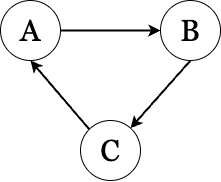
\includegraphics[width=0.6\textwidth,height=\textheight]{img/original_DCG.png}

}

\subcaption{\label{fig-examplegraphs-1}Example graph \(\mathcal{G}\)}

\end{minipage}%
%
\begin{minipage}{0.33\linewidth}

\centering{

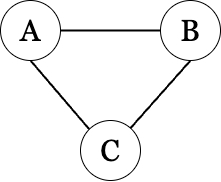
\includegraphics[width=0.6\textwidth,height=\textheight]{img/FCI_graph.png}

}

\subcaption{\label{fig-examplegraphs-2}Corresponding MAAG}

\end{minipage}%
%
\begin{minipage}{0.33\linewidth}

\centering{

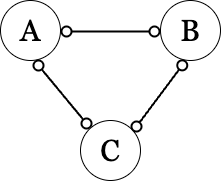
\includegraphics[width=0.6\textwidth,height=\textheight]{img/CCI_graph.png}

}

\subcaption{\label{fig-examplegraphs-3}Corrsponding PAG}

\end{minipage}%

\caption{\label{fig-examplegraphs}Example graph \(\mathcal{G}\)
featuring a cycle and the corresponding MAAG from CCI and PAG from FCI.}

\end{figure}%

The graph produced by the PC algorithm is a \emph{CPDAG} (completed
partially directed acyclic graph), where directed edges (\(A\) → \(B\))
indicate that \(A\) is a direct cause (parent) of \(B\). Unlike FCI and
CCI, the CPDAG does not include circle symbols. Instead, when the PC
algorithm cannot determine the direction of causality, it represents
this uncertainty with bidirectional arrows. While the PC algorithm
serves as a useful reference, its strict assumptions --- acyclicity and
the absence of latent confounders---limit its applicability in more
complex scenarios. For this reason, our primary focus remains on the
results obtained from FCI and CCI, with all PC algorithm results
provided in Section~\ref{sec-pc} for completeness.

\subsection{Precariousness Domains Based on Elsenburg et
al.~(2025)}\label{precariousness-domains-based-on-elsenburg-et-al.-2025}

\begin{enumerate}
\def\labelenumi{\arabic{enumi}.}
\tightlist
\item
  EMPLOYMENT PRECARIOUSNESS
\end{enumerate}

\begin{itemize}
\tightlist
\item
  \texttt{H1\_Arbeidsparticipatie}: Working status
\item
  \texttt{H1\_WerkSit}: Which work situation most applies to you?
\item
  \texttt{H1\_RecentErv8}: Experiences past 12 months: h. You were
  sacked from your job or became unemployed (\emph{reverse})
\end{itemize}

\begin{enumerate}
\def\labelenumi{\arabic{enumi}.}
\setcounter{enumi}{1}
\tightlist
\item
  FINANCIAL PRECARIOUSNESS
\end{enumerate}

\begin{itemize}
\tightlist
\item
  \texttt{H1\_InkHhMoeite}: During the past year, did you have problems
  managing your household income?
\item
  \texttt{H1\_RecentErv9}: Experiences past 12 months: i. You had a
  major financial crisis (\emph{reverse})
\end{itemize}

\begin{enumerate}
\def\labelenumi{\arabic{enumi}.}
\setcounter{enumi}{2}
\tightlist
\item
  HOUSING PRECARIOUSNESS
\end{enumerate}

\begin{itemize}
\tightlist
\item
  \texttt{veilig\_2012}: Score safety (veiligheid) in 2012
  (\emph{reverse})
\item
  \texttt{vrz\_2012}: Score level of resources (niveau voorzieningen) in
  2012 (\emph{reverse})
\item
  \texttt{P\_HUURWON}: Percentage Huurwoningen
\end{itemize}

\begin{enumerate}
\def\labelenumi{\arabic{enumi}.}
\setcounter{enumi}{3}
\tightlist
\item
  CULTURAL PRECARIOUSNESS
\end{enumerate}

\begin{itemize}
\tightlist
\item
  \texttt{H1\_Discr\_sumscore}: Perceived discrimination: sum score of 9
  items (range 9-45)
\item
  \texttt{H1\_SBSQ\_meanscore}: Health literacy: SBSQ meanscore (range
  1-5) (\emph{reverse})
\item
  \texttt{A\_BED\_RU}: Aantal bedrijfsvestigingen; cultuur, recreatie,
  overige diensten (\emph{reverse})
\end{itemize}

\begin{enumerate}
\def\labelenumi{\arabic{enumi}.}
\setcounter{enumi}{4}
\tightlist
\item
  SOCIAL PRECARIOUSNESS
\end{enumerate}

\begin{itemize}
\tightlist
\item
  \texttt{H1\_RecentErv5}: Experiences past 12 months: e. Your steady
  relationship ended (\emph{reverse})
\item
  \texttt{H1\_RecentErv6}: Experiences past 12 months: f.~A long-term
  friendship with a good friend or family member was broken off
  (\emph{reverse})
\item
  \texttt{H1\_RecentErv7}: Experiences past 12 months: g. You had a
  serious problem with a good friend or family member, or neighbour
  (\emph{reverse})
\item
  \texttt{H1\_SSQT}: SSQT (frequency of social contact): sum score of 5
  items (range 5-20) (\emph{reverse})
\item
  \texttt{H1\_SSQSa}: SSQS (adequacy of social contact): sum score of 5
  items, category 3 and 4 not combined (range 5-20) (\emph{reverse})
\end{itemize}

\begin{center}
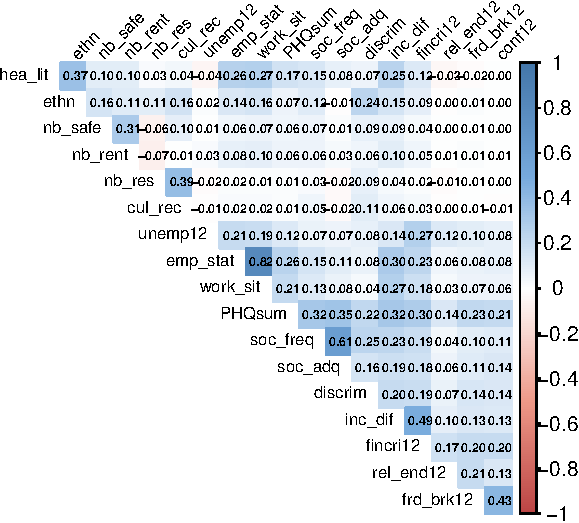
\includegraphics{draft_v2_files/figure-pdf/unnamed-chunk-12-1.pdf}
\end{center}

\begin{itemize}
\item
  \textbf{High} Correlations: \texttt{emp\_stat} (employment status) and
  \texttt{work\_sit} (work situation) have a strong positive correlation
  of 0.82. This suggests that individuals with higher employment status
  tend to have more secure or favorable work situations.
  \texttt{soc\_freq} (social contact frequency) shows a strong positive
  correlation with \texttt{soc\_adq} (social adequacy) at 0.61. This
  indicates that individuals with more frequent social contact also tend
  to have higher perceived adequacy of social interactions.
\item
  \textbf{Moderate} Correlations: \texttt{nb\_safe} (neighborhood
  safety) and \texttt{nb\_res} (resources) have a moderate positive
  correlation of 0.39, suggesting that areas with higher safety also
  have better resources. \texttt{hea\_lit} (health literacy) has
  moderate correlations with \texttt{emp\_stat} (0.26) and
  \texttt{work\_sit} (0.25), which could mean that higher health
  literacy is associated with better employment situations.
  \texttt{frd\_brk12} (friendship breakups) and \texttt{conf12}
  (conflicts) have a notable correlation of 0.43, indicating a
  relationship between having conflicts and friendship losses.
\item
  \textbf{Low to Moderate} Correlations in Financial Precariousness:
  \texttt{inc\_dif} (income difficulties) has a moderate correlation
  with \texttt{fincri12} (financial crisis) at 0.49. This aligns with
  the expected relationship, where individuals who experience general
  income difficulties are more likely to report financial crises.
\item
  \textbf{Low} Correlations (0.1 - 0.2): Many variables, such as
  \texttt{discrim} (discrimination), \texttt{unemp12} (unemployment
  experience), and \texttt{rel\_end12} (relationship end), have low
  correlations with other variables, suggesting relatively independent
  relationships in the context of this dataset.
\end{itemize}

\subsubsection{Exploratory Factor Analysis
(EFA)}\label{exploratory-factor-analysis-efa}

\begin{center}
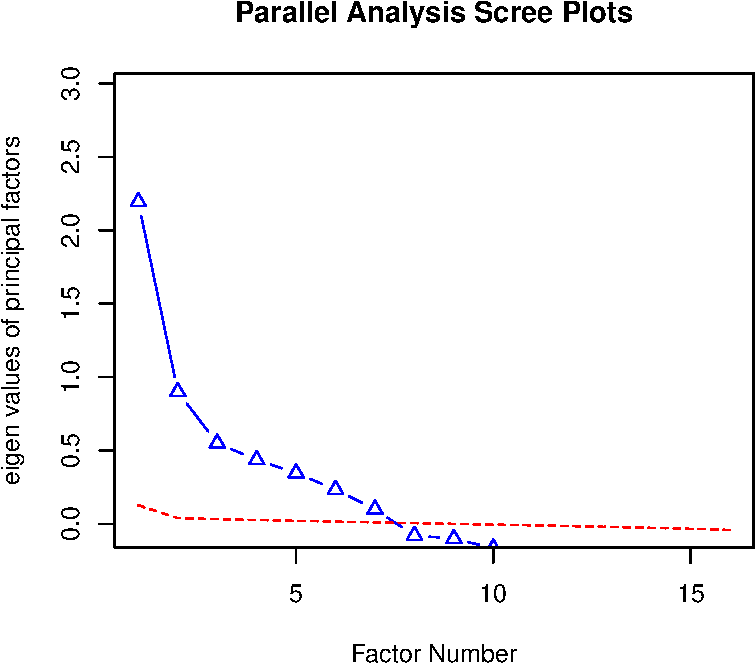
\includegraphics[width=0.55\textwidth,height=\textheight]{draft_v2_files/figure-pdf/unnamed-chunk-13-1.pdf}
\end{center}

\begin{center}
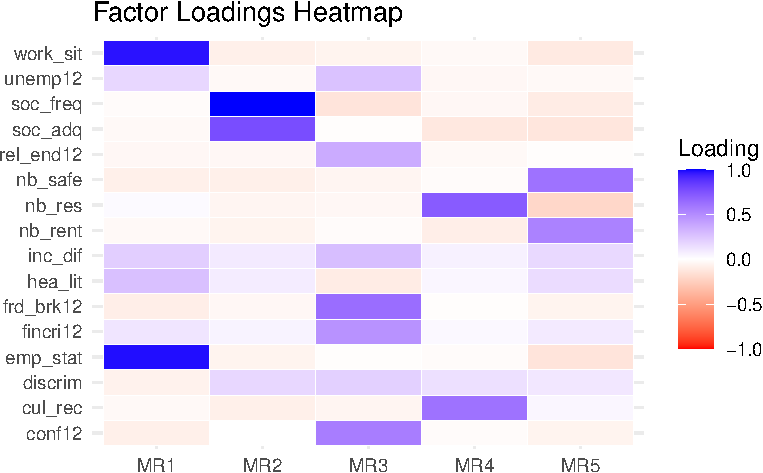
\includegraphics[width=0.7\textwidth,height=\textheight]{draft_v2_files/figure-pdf/unnamed-chunk-14-1.pdf}
\end{center}

\paragraph{Factor Loadings (Pattern
Matrix)}\label{factor-loadings-pattern-matrix}

\begin{itemize}
\tightlist
\item
  \textbf{MR1}: High loadings on \texttt{emp\_stat} and
  \texttt{work\_sit} suggest this factor captures \emph{employment}
  precariousness.
\item
  \textbf{MR2}: Strong loadings on \texttt{soc\_freq} and
  \texttt{soc\_adq} indicate \emph{social} precariousness.
\item
  \textbf{MR3}: Key items like \texttt{frd\_brk12}, \texttt{conf12}, and
  \texttt{fincri12}, suggest recent \emph{stressful events}.
\item
  \textbf{MR4}: High loadings on \texttt{nb\_res} and \texttt{cul\_rec}
  may reflect \emph{community resources} precariousness.
\item
  \textbf{MR5}: Variables \texttt{nb\_safe} and \texttt{nb\_rent} with
  high loadings indicate \emph{housing} precariousness.
\end{itemize}

\paragraph{Variance Explained}\label{variance-explained}

The factors cumulatively explain \textbf{38\%} of the variance, with MR1
being the most influential factor. Each factor contributes a smaller
proportion to the total variance (MR1 at 12\%, MR2 at 9\%, etc.).

\paragraph{Factor Intercorrelations}\label{factor-intercorrelations}

Factors are moderately correlated, especially between \emph{MR1 and
MR5}, and \emph{MR2 and MR3}. This indicates that while distinct, these
factors are related---reasonable in a complex socio-economic context.

\paragraph{Model Fit Statistics}\label{model-fit-statistics}

RMSEA (0.071) suggest an acceptable fit. Tucker Lewis Index (0.802)
suggests moderate reliability for the model.

\paragraph{Summary}\label{summary}

The 5-factor model appears interpretable and captures distinct
dimensions of precariousness: \emph{employment, social, stressors,
community resources, and housing precariousness}. Although the overall
fit and explained variance could be stronger, these factors offer
insights into the underlying structure of the data, highlighting key
areas of precariousness.

\subsubsection{PCA}\label{pca}

\begin{center}
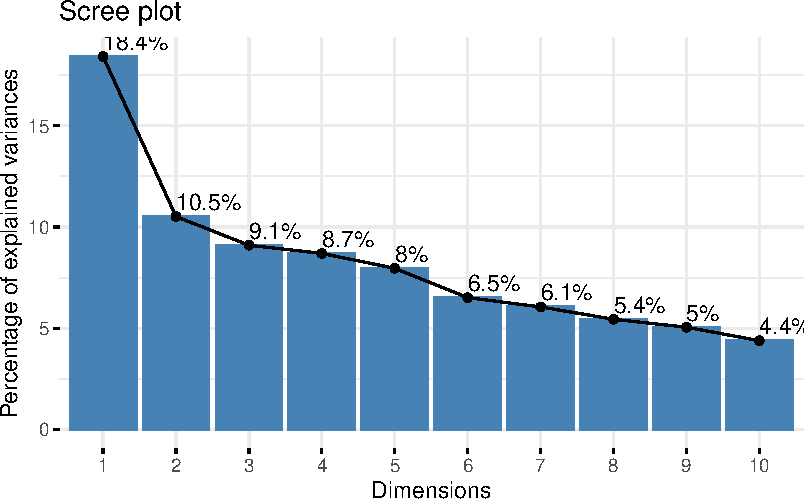
\includegraphics[width=0.7\textwidth,height=\textheight]{draft_v2_files/figure-pdf/unnamed-chunk-15-1.pdf}
\end{center}

\begin{itemize}
\tightlist
\item
  Component Retention: The scree plot shows a clear ``elbow'' after the
  first component. This steep drop suggests that most variance is
  explained by the first component. After Dimension 5, the percentage of
  explained variance decreases slightly more gradually, indicating
  diminishing returns for adding more components. If we need to choose
  multiple components, retaining the first 5 components seems
  reasonable, as they capture most of the variance (cumulatively
  explaining about 54.7\% of the total variance).
\end{itemize}

\begin{center}
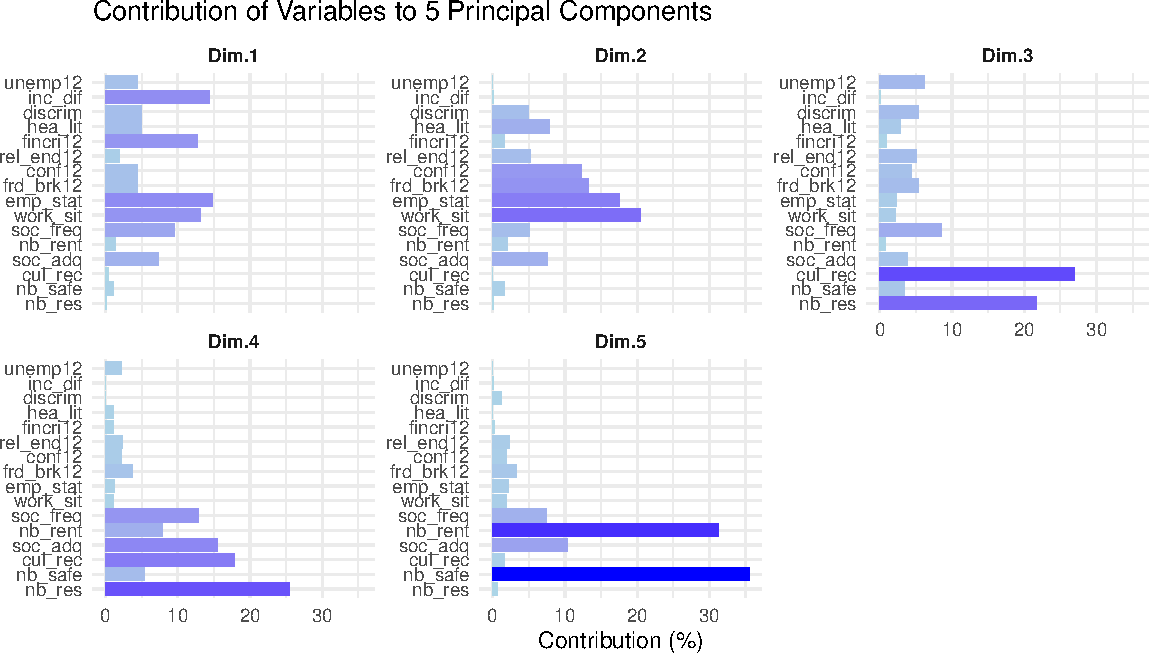
\includegraphics{draft_v2_files/figure-pdf/unnamed-chunk-16-1.pdf}
\end{center}

\paragraph{Explained variance (contributions) of
variables}\label{explained-variance-contributions-of-variables}

It shows the importance of variables within each component.

\begin{itemize}
\item
  \textbf{Dim1}: High contributions are observed from
  \texttt{emp\_stat}, \texttt{work\_sit}, \texttt{inc\_dif}, and
  \texttt{fincri12}, suggesting that this dimension captures aspects of
  \emph{employment and financial} security.
\item
  \textbf{Dim2}: While \texttt{emp\_stat} and \texttt{work\_sit} overlap
  with Dim1, the strong contributions from \texttt{frd\_brk12} and
  \texttt{rel\_end12} indicate that this dimension captures a focus on
  \emph{recent relationship stressors}.
\item
  \textbf{Dim3}: \texttt{cul\_rec}, \texttt{nb\_res} have the highest
  contributions, indicating this dimension likely represents
  \emph{community and cultural} factors.
\item
  \textbf{Dim4}: \texttt{soc\_freq} and \texttt{soc\_adq} stand out in
  this dimension, suggesting an emphasis on \emph{social}
  precariousness.
\item
  \textbf{Dim5}: \texttt{nb\_safe} and \texttt{nb\_rent} are the top
  contributors, pointing to \emph{housing} security as key themes in
  this component.
\end{itemize}

\paragraph{Cos² Values}\label{cosuxb2-values}

Cos² (squared cosine) values, or the quality of representation, show how
well each variable is represented by each dimension. where higher cos²
values (closer to 1) indicate better representation of a variable by a
component.

\begin{center}
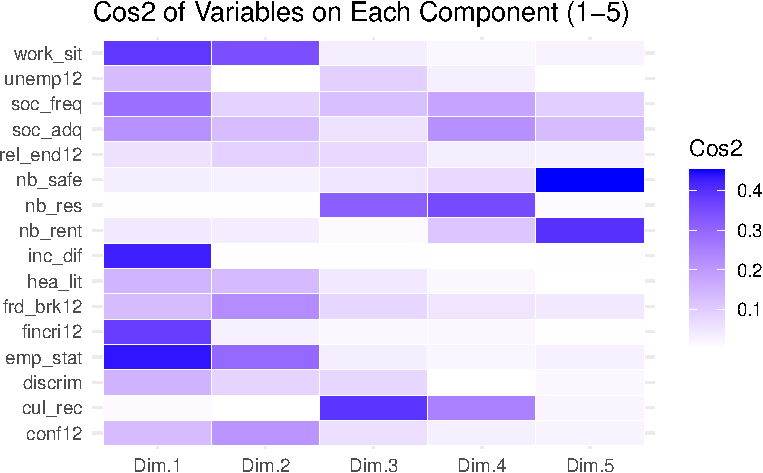
\includegraphics[width=0.7\textwidth,height=\textheight]{draft_v2_files/figure-pdf/unnamed-chunk-17-1.pdf}
\end{center}

\begin{itemize}
\item
  \textbf{Dim.1}: Variables \texttt{emp\_stat}, \texttt{work\_sit},
  \texttt{inc\_dif}, and \texttt{fincri12} show high cos² values,
  meaning that PC1 primarily captures variations in employment and
  financial difficulties. This component could represent
  \emph{employment \& finance} precariousness.
\item
  \textbf{Dim.2}: Variables \texttt{work\_sit}, \texttt{emp\_stat},
  \texttt{frd\_brk12}, and \texttt{conf12} are well-represented in this
  component, suggesting PC2 captures aspects of \emph{recent
  relationship stressors}.
\item
  \textbf{Dim.3}: Variables \texttt{nb\_res} and \texttt{cul\_rec} load
  strongly on PC3. This may represent community or cultural resources,
  indicating that this component is associated with \emph{neighborhood
  resources}.
\item
  \textbf{Dim.4}: This component has high cos² values for
  \texttt{nb\_res}, \texttt{cul\_rec}, \texttt{soc\_freq}, and
  \texttt{soc\_adq.} While \texttt{nb\_res} and \texttt{cul\_rec} are
  also prominent in PC3, PC4 uniquely captures nuanced differentiation
  in \emph{social} precariousness.
\item
  \textbf{Dim.5}: \texttt{nb\_safe} and \texttt{nb\_rent} are
  well-represented by PC5. This component might capture \emph{housing}
  precariousness.
\end{itemize}

\subsubsection{ICA}\label{ica}

\begin{center}
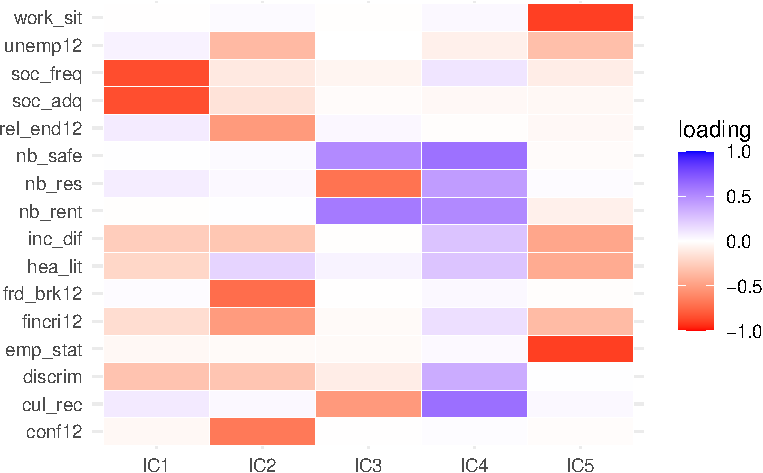
\includegraphics[width=0.7\textwidth,height=\textheight]{draft_v2_files/figure-pdf/unnamed-chunk-18-1.pdf}
\end{center}

\paragraph{Dominant Variables per
Component:}\label{dominant-variables-per-component}

For each Independent Component (IC), we can identify variables with
\emph{high absolute} values in each column. These values indicate that
the IC captures a strong, independent signal associated with these
variables.

\begin{itemize}
\item
  \textbf{IC1}: \texttt{soc\_freq} and \texttt{soc\_adq} have strong
  negative loadings on this component, indicating that this component
  might represent \emph{social} precariousness.
\item
  \textbf{IC2}: \texttt{frd\_brk12}, \texttt{conf12},
  \texttt{rel\_end12}, \texttt{fincri12} and \texttt{unemp12} have the
  most substantial loadings on this component, all with negative signs.
  This might point to a \emph{recent relational or social stressor}
  component.
\item
  \textbf{IC3}: \texttt{nb\_res} and \texttt{cul\_rec} show notable
  negative loadings, pointing to a focus on \emph{community resource}
  precariousness.
\item
  \textbf{IC4}: High loadings for \texttt{nb\_safe}, \texttt{nb\_rent},
  \texttt{nb\_res}, \texttt{cul\_rec}, and \texttt{discrim} suggest a
  theme of \emph{housing and community-based} precariousness, reflecting
  both safety and social challenges within the neighborhood context.
\item
  \textbf{IC5}: \texttt{emp\_stat} and \texttt{work\_sit} both have
  strong negative loadings on this component, suggesting it captures
  \emph{employment} precariousness.
\end{itemize}

\subsubsection{Hierarchical clustering}\label{hierarchical-clustering}

\paragraph{Using Euclidean distance}\label{using-euclidean-distance}

\begin{itemize}
\tightlist
\item
  Ward.D's method: Minimizes the variance within clusters, producing
  more compact and spherical clusters.
\item
  Single linkage: Groups clusters based on the minimum distance between
  points.
\item
  Complete linkage: Groups clusters based on the maximum distance
  between points.
\item
  Average linkage: Uses the average distance between all pairs of points
  in the two clusters.
\end{itemize}

\begin{figure}

\begin{minipage}{0.50\linewidth}
\begin{center}
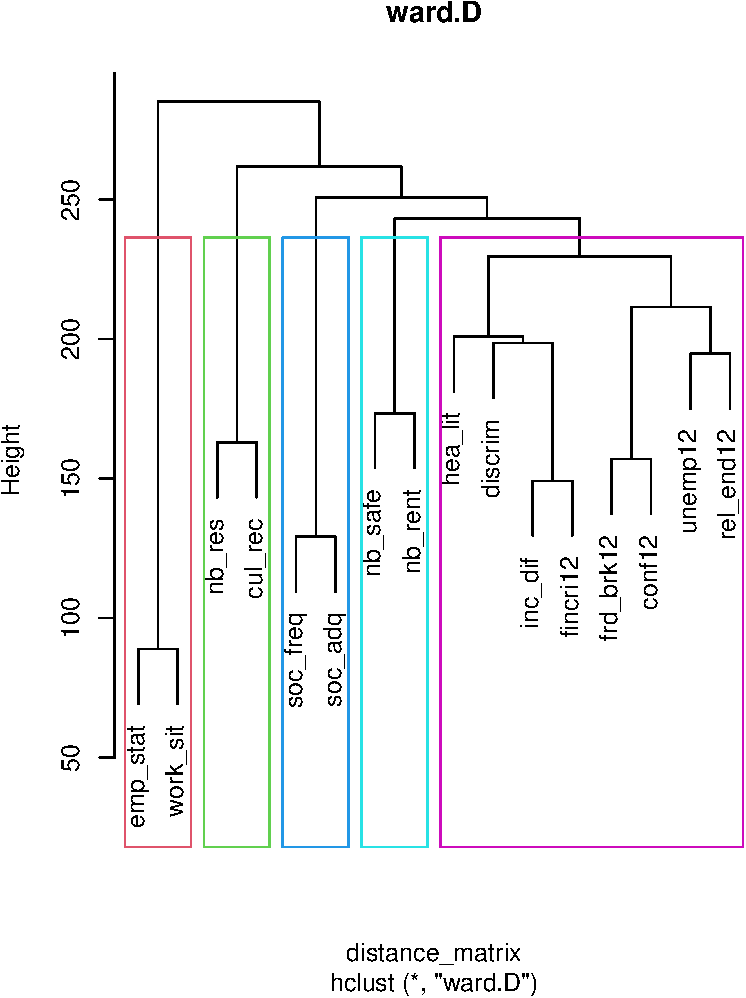
\includegraphics{draft_v2_files/figure-pdf/unnamed-chunk-19-1.pdf}
\end{center}
\end{minipage}%
%
\begin{minipage}{0.50\linewidth}
\begin{center}
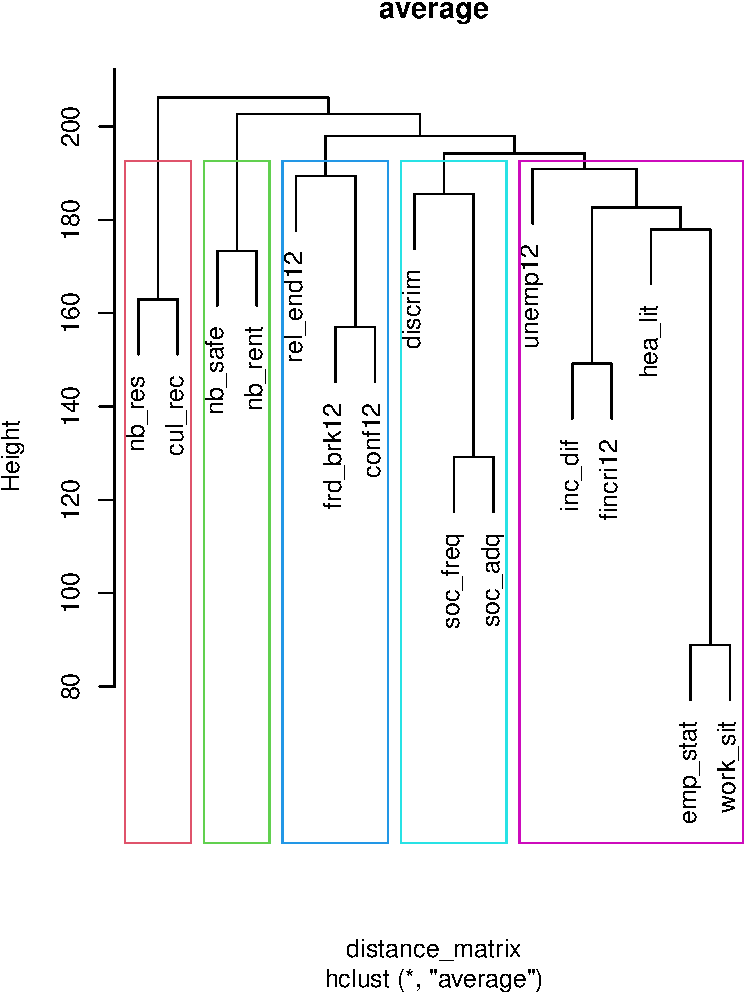
\includegraphics{draft_v2_files/figure-pdf/unnamed-chunk-19-2.pdf}
\end{center}
\end{minipage}%
\newline
\begin{minipage}{0.50\linewidth}
\begin{center}
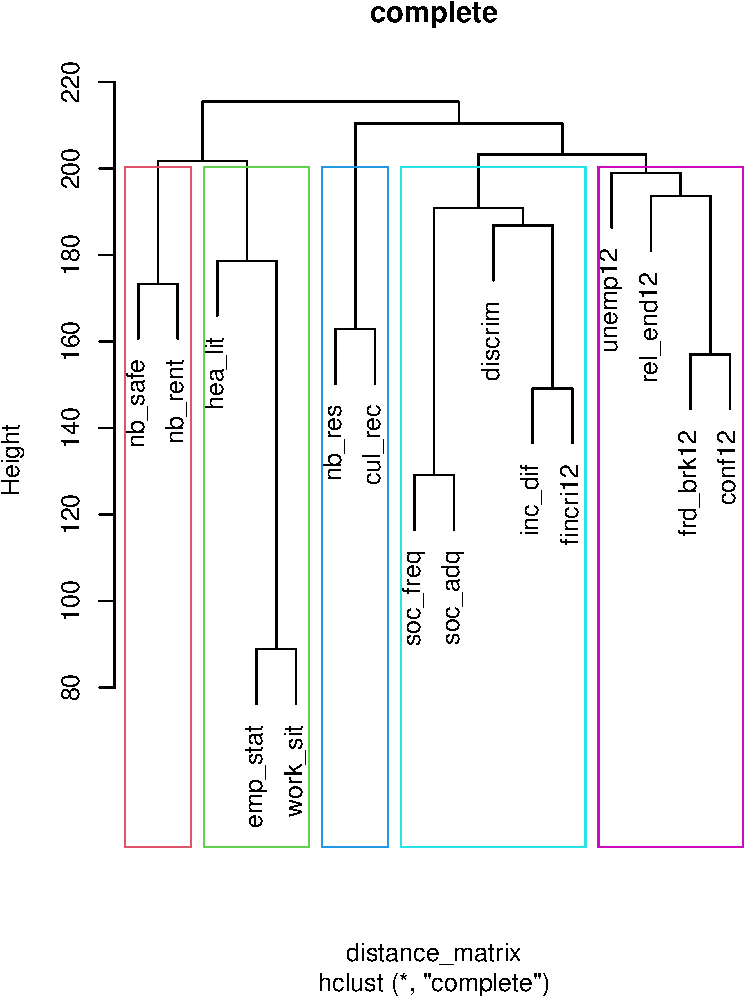
\includegraphics{draft_v2_files/figure-pdf/unnamed-chunk-19-3.pdf}
\end{center}
\end{minipage}%
%
\begin{minipage}{0.50\linewidth}
\begin{center}
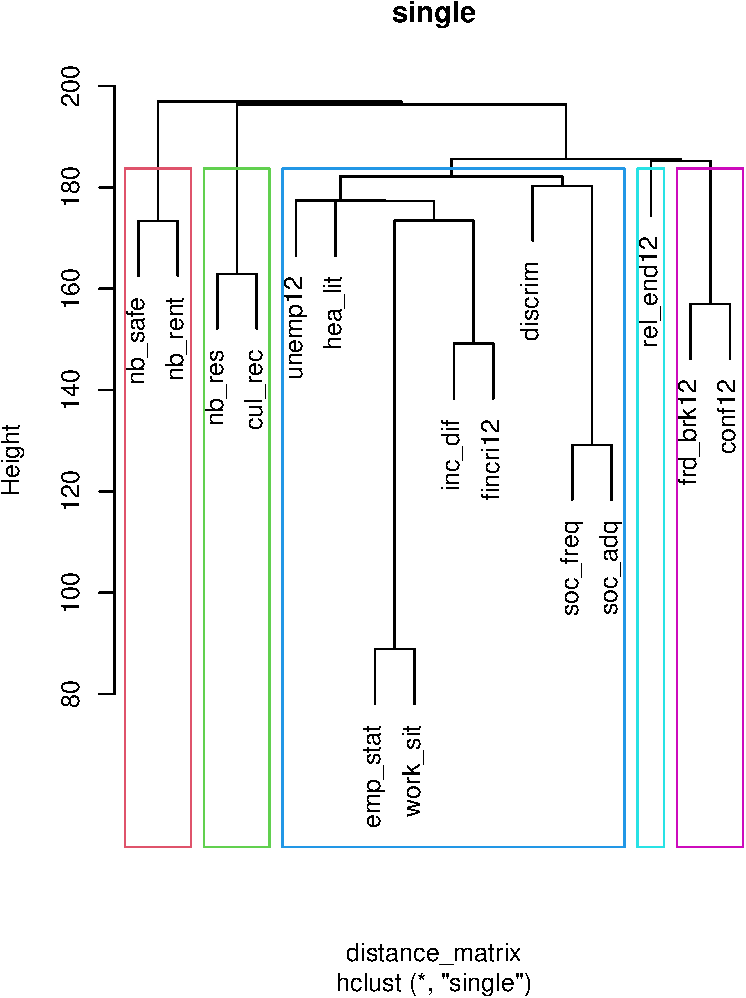
\includegraphics{draft_v2_files/figure-pdf/unnamed-chunk-19-4.pdf}
\end{center}
\end{minipage}%

\end{figure}%

\subparagraph{Consistent Groupings (Across All or Most
Methods)}\label{consistent-groupings-across-all-or-most-methods}

\begin{itemize}
\item
  \texttt{emp\_stat} and \texttt{work\_sit}: This pair consistently
  clusters together across all linkage methods, suggesting that they are
  closely related variables, likely capturing a similar aspect of the
  data (possibly employment status or employment-related information).
\item
  \texttt{nb\_safe}, \texttt{nb\_res}, and \texttt{nb\_rent}: These
  variables are often grouped closely in several methods (especially
  Ward.D, average, and complete linkage). This suggests a similarity or
  common theme among them, potentially related to neighborhood or
  housing precariousness.
\item
  \texttt{soc\_freq} and \texttt{soc\_adq}: These two variables
  frequently cluster together, indicating they likely measure aspects of
  social frequency and adequacy in similar ways. They appear together in
  Ward.D, average, and complete linkage.
\item
  \texttt{frd\_brk12} and \texttt{conf12}: These variables are often
  clustered closely (though they sometimes join with other variables
  like rel\_end12), suggesting they may capture aspects of relationship
  or social conflict. This pair appears in close proximity, especially
  in average and Ward.D.
\end{itemize}

\subparagraph{Inconsistent Groupings (Variability Across
Methods)}\label{inconsistent-groupings-variability-across-methods}

\begin{itemize}
\item
  \texttt{hea\_lit}: This variable shows inconsistent clustering across
  methods. In Ward.D, it joins with \texttt{fincri12}, while in other
  methods, it's often more isolated or grouped with variables that do
  not appear similar. This may suggest that \texttt{hea\_lit} does not
  strongly correlate with other variables, or it has multidimensional
  aspects affecting its grouping across methods.
\item
  \texttt{discrim}: This variable also shows variable groupings. In
  Ward.D, it is grouped with \texttt{hea\_lit}, while in other methods
  (e.g., complete and single linkage), it clusters differently,
  sometimes on its own. This variability may indicate that
  \texttt{discrim} has weaker associations with the main clusters in the
  data or overlaps partially with multiple clusters.
\item
  Social and Financial Variables (\texttt{inc\_dif}, \texttt{fincri12},
  \texttt{unemp12}): These variables appear together in some methods
  (e.g., Ward.D clusters \texttt{fincri12} and \texttt{inc\_dif}), but
  in others, they are spread out. This inconsistency suggests that
  social and financial variables may not have strong or consistent ties
  across different methods, perhaps due to capturing different aspects
  of precariousness.
\end{itemize}

\subparagraph{Summary}\label{summary-1}

The consistent clusters are likely capturing distinct thematic
dimensions of the data (e.g., employment, housing, social contact),
while the inconsistent variables may reflect multifaceted or weakly
correlated attributes that do not fit neatly into one cluster.

\paragraph{Using Mutual Information}\label{using-mutual-information}

Using mutual information (MI) as a basis for hierarchical clustering
differs from using traditional distance measures (like Euclidean
distance) in a few key ways.

\begin{center}
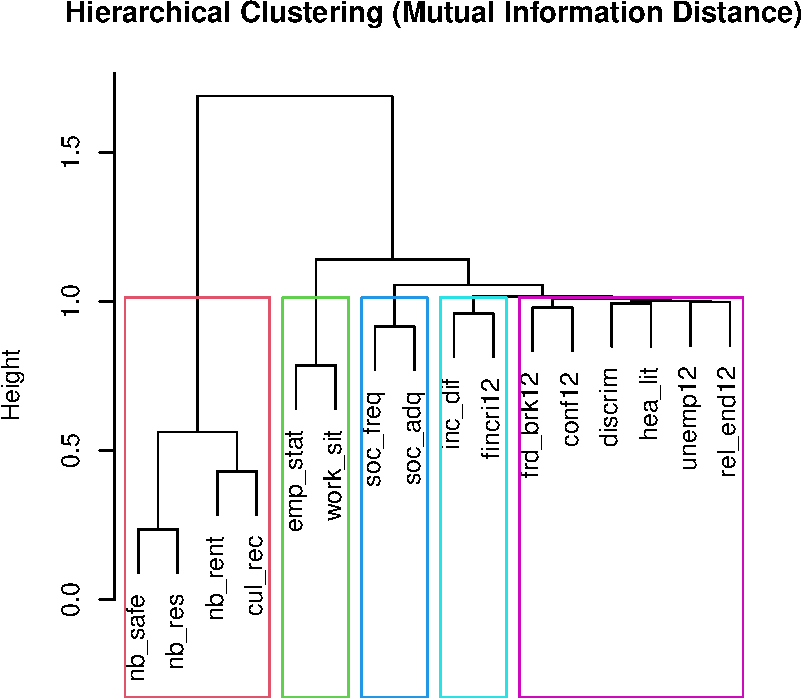
\includegraphics[width=0.6\textwidth,height=\textheight]{draft_v2_files/figure-pdf/unnamed-chunk-20-1.pdf}
\end{center}

\subparagraph{Comparison to Euclidean Distance
Clustering}\label{comparison-to-euclidean-distance-clustering}

\begin{itemize}
\item
  \textbf{Housing and Community} Cluster: The variables
  \texttt{nb\_safe}, \texttt{nb\_res}, \texttt{nb\_rent}, and
  \texttt{cul\_rec} cluster together, indicating a strong association
  among housing-related and community-based factors. This suggests a
  shared theme of housing or community precariousness. This grouping is
  also observed in the Euclidean-based clustering, but it appears more
  tightly connected here, potentially due to the non-linear
  relationships highlighted by mutual information.
\item
  \textbf{Employment and Social Support} Cluster: \texttt{emp\_stat} and
  \texttt{work\_sit} form a cluster, linking employment status and work
  situation together as they did in Euclidean-based clustering. These
  remain closely associated regardless of the distance metric used.
  \texttt{soc\_freq} and \texttt{soc\_adq}, related to social contact
  frequency and adequacy, cluster nearby, indicating they have a
  stronger non-linear relationship with employment variables. This is a
  subtle difference as Euclidean distance might not capture this
  association as effectively.
\item
  \textbf{Financial Stressor} Cluster: \texttt{inc\_dif} and
  \texttt{fincri12}, representing income difficulties and recent
  financial crises, consistently cluster together in both approaches,
  showing a strong association, likely linear. However, mutual
  information-based clustering links these financial stressors with
  social support variables, suggesting that financial challenges may
  have complex dependencies with social support in this dataset.
\item
  \textbf{Relational Stressor} Cluster: \texttt{frd\_brk12},
  \texttt{conf12}, \texttt{discrim}, \texttt{hea\_lit},
  \texttt{unemp12}, and \texttt{rel\_end12} form a \emph{looser} cluster
  focused on social and relational stressors (e.g., friendship breakup,
  conflicts, and discrimination). Compared to Euclidean clustering,
  \texttt{discrim} and \texttt{hea\_lit} (health literacy) appear closer
  to relational stressors here, indicating that non-linear relationships
  might play a larger role in linking these variables.
\end{itemize}

\subparagraph{Summary}\label{summary-2}

In conclusion, mutual information-based clustering provides an
alternative perspective that can reveal more intricate associations
between variables, especially for those with non-linear relationships.
Compared to Euclidean clustering, it shows a similar high-level
structure but emphasizes nuanced connections between variables,
particularly around social support, employment, and financial stress.

\subsubsection{Conclusions on Precariousness
factors}\label{conclusions-on-precariousness-factors}

Based on the consistent findings across multiple analyses, we decided to
exclude the variables \texttt{discrim}, \texttt{hea\_lit},
\texttt{umemp12}, and \texttt{rel\_end12}, as they do not clearly belong
to any specific precariousness factor nor exhibit strong associations
with depression (see the correlation table above). Therefore, we propose
retaining the following key precariousness factors:

\begin{itemize}
\tightlist
\item
  Employment Precariousness: \texttt{emp\_stat}, \texttt{work\_sit}
\item
  Social Precariousness: \texttt{soc\_freq}, \texttt{soc\_adq}
\item
  Housing Precariousness: \texttt{nb\_safe}, \texttt{nb\_res},
  \texttt{nb\_rent}, \texttt{cul\_rec}
\item
  Recent Relational Stressors: \texttt{frd\_brk12}, \texttt{conf12}
\item
  Recent Financial Stressors: \texttt{fincri12}, \texttt{inc\_diff}
\end{itemize}

We construct each precariousness factor by calculating the mean value of
the combined variables. Below, we present the updated correlation table
for the newly composed factors, along with the corresponding
distributions of all variables to be used in the causal discovery
analysis.

\begin{center}
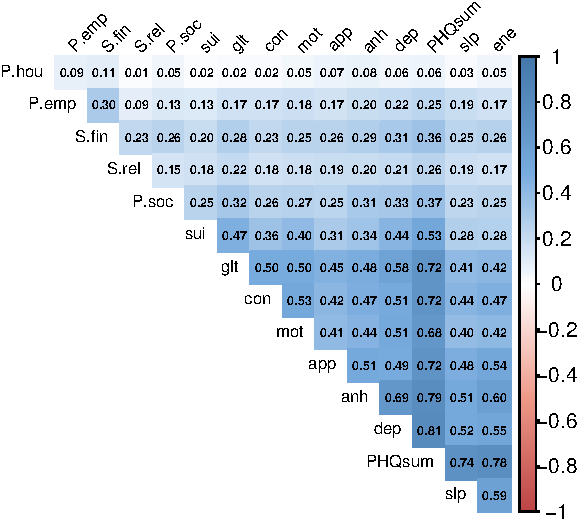
\includegraphics{draft_v2_files/figure-pdf/unnamed-chunk-21-1.pdf}
\end{center}

\begin{center}
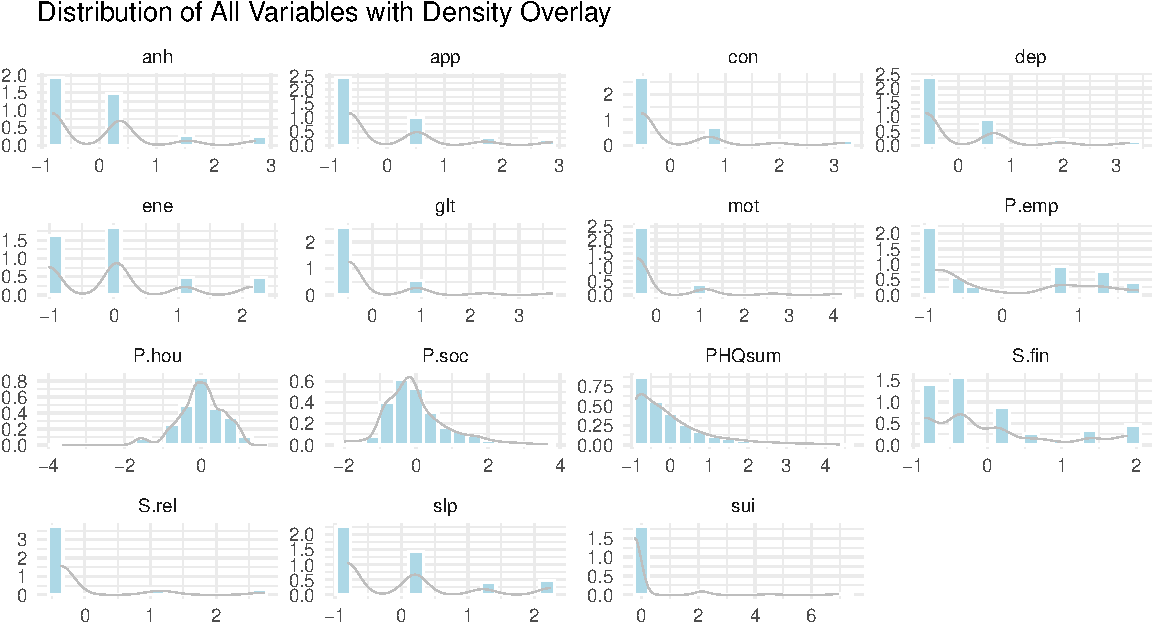
\includegraphics{draft_v2_files/figure-pdf/unnamed-chunk-22-1.pdf}
\end{center}

\subsection{Results from CCI algorithm}\label{sec-cci}

\begin{figure}

\begin{minipage}{0.50\linewidth}

\centering{

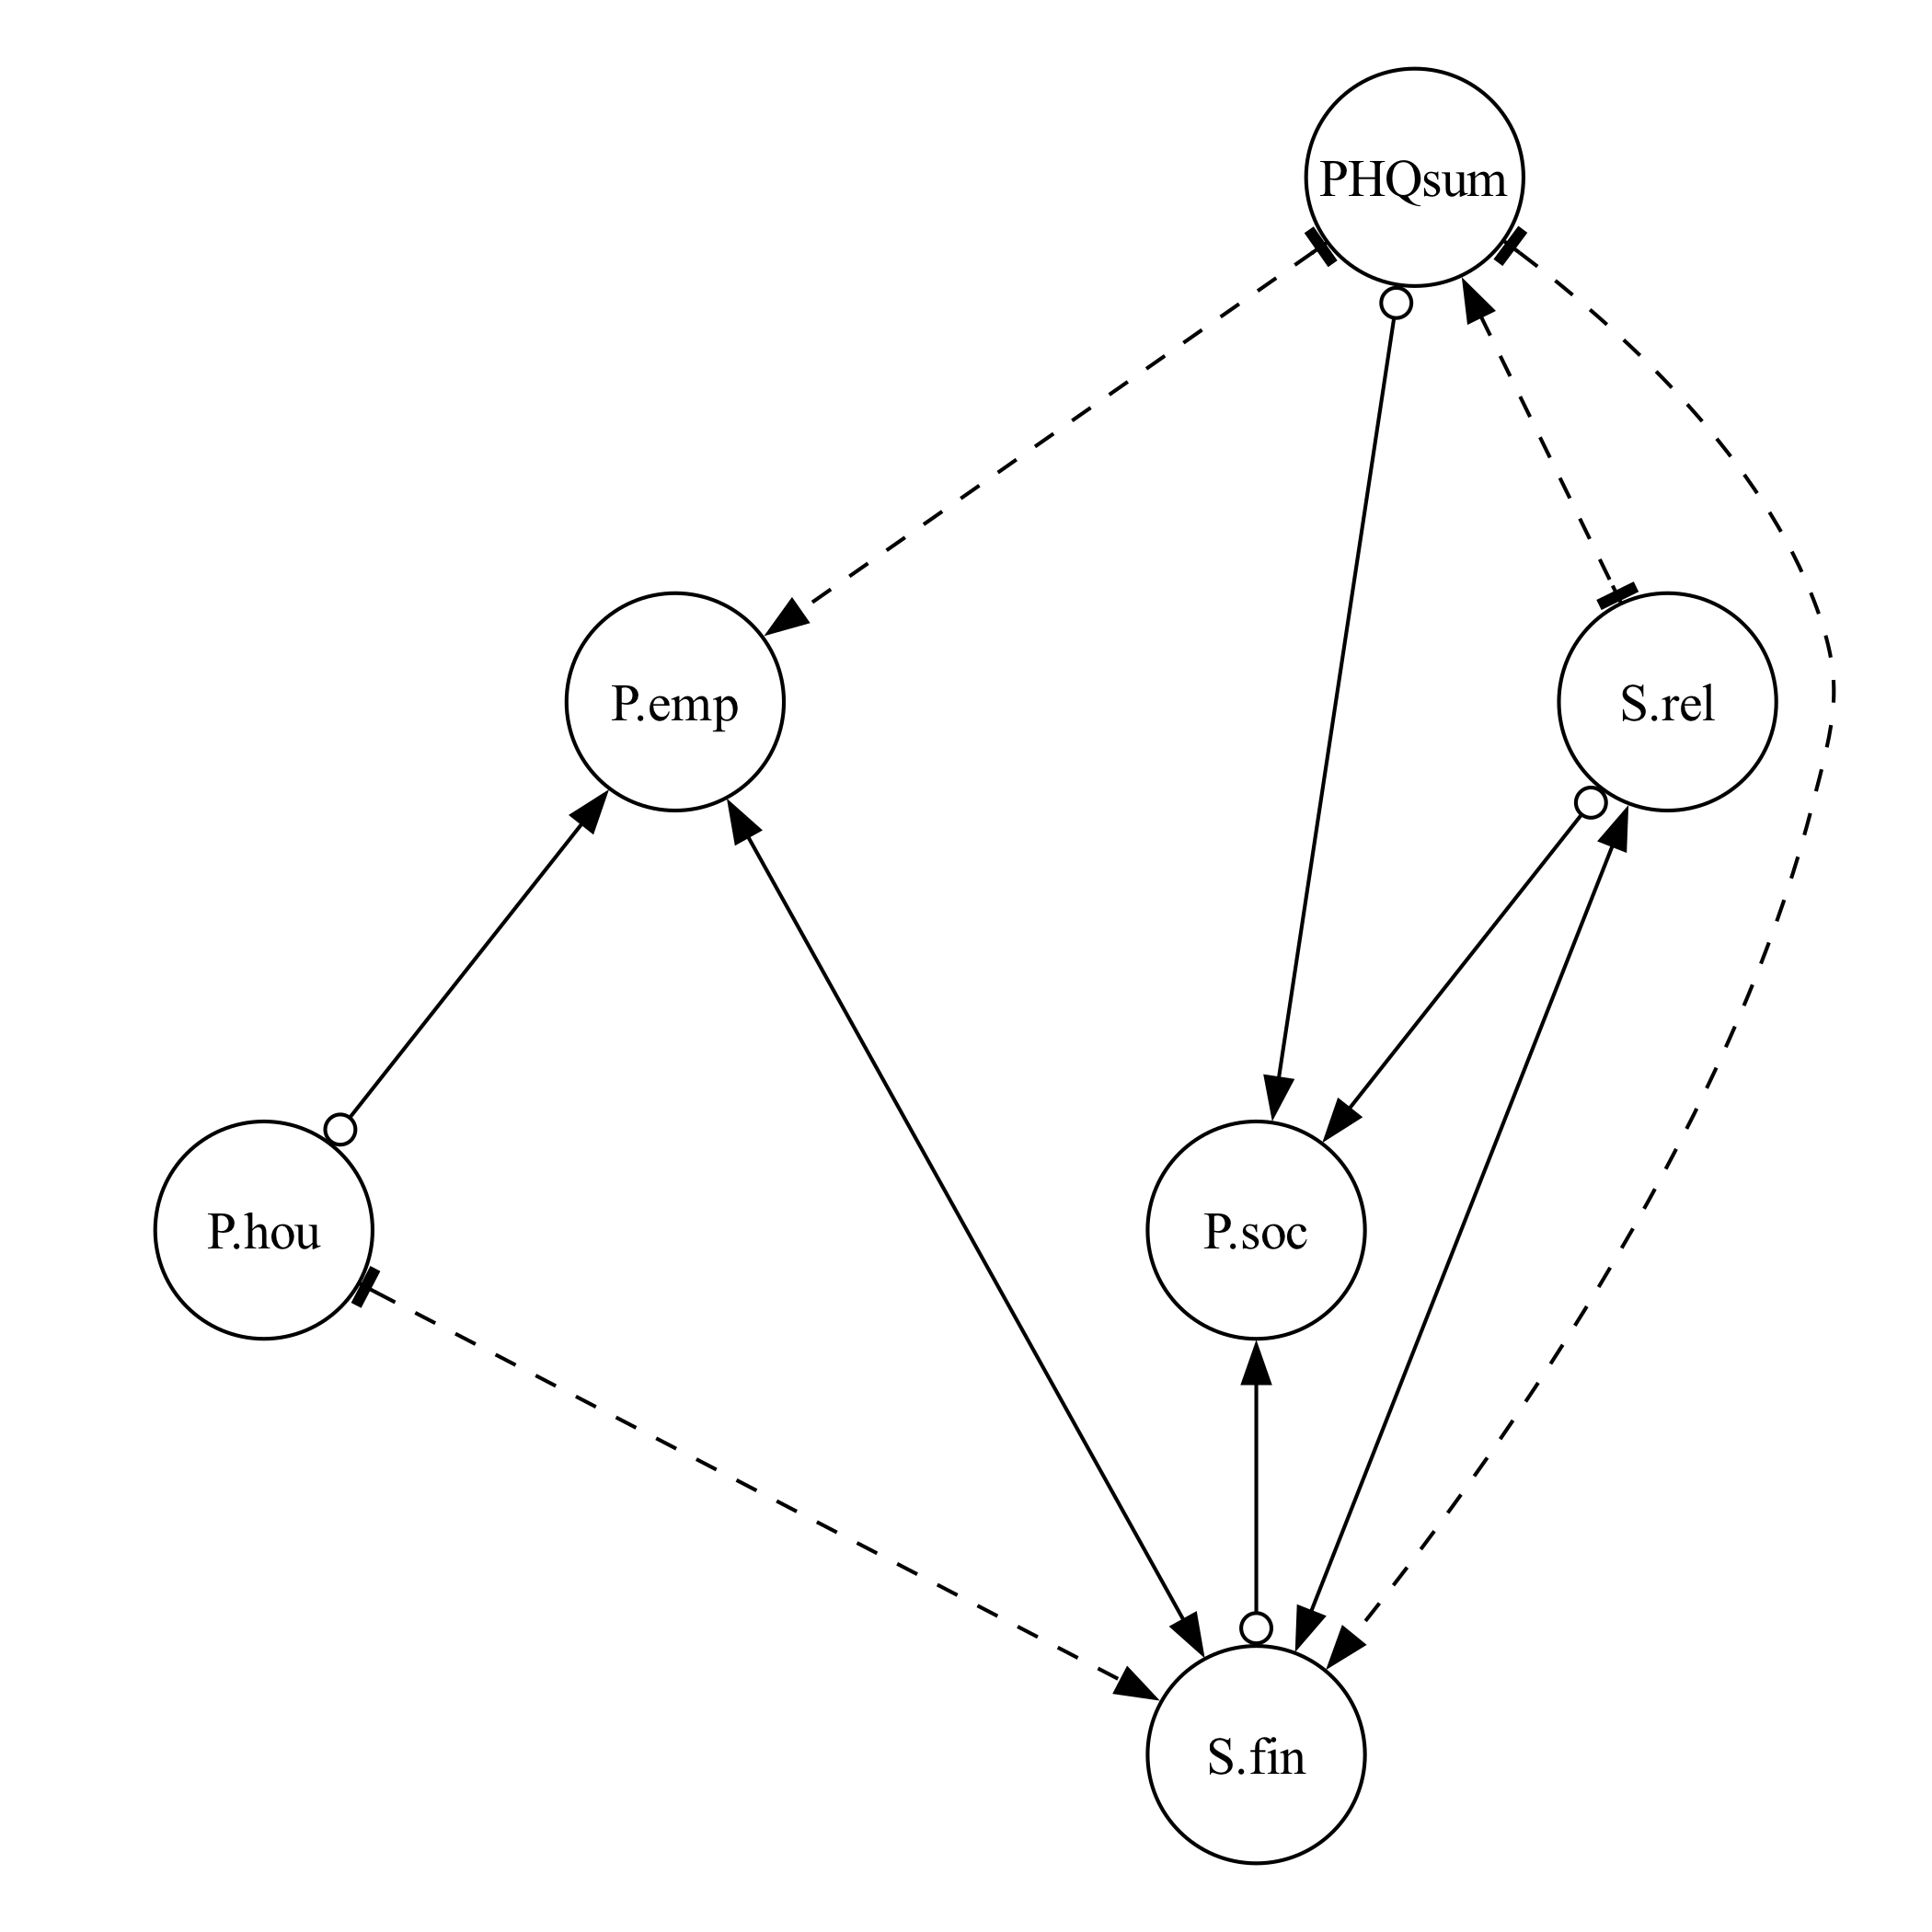
\includegraphics[width=1\textwidth,height=\textheight]{img/CCI_depsum.png}

}

\subcaption{\label{fig-sum-cci-1}CCI MAAG}

\end{minipage}%
%
\begin{minipage}{0.50\linewidth}

\centering{

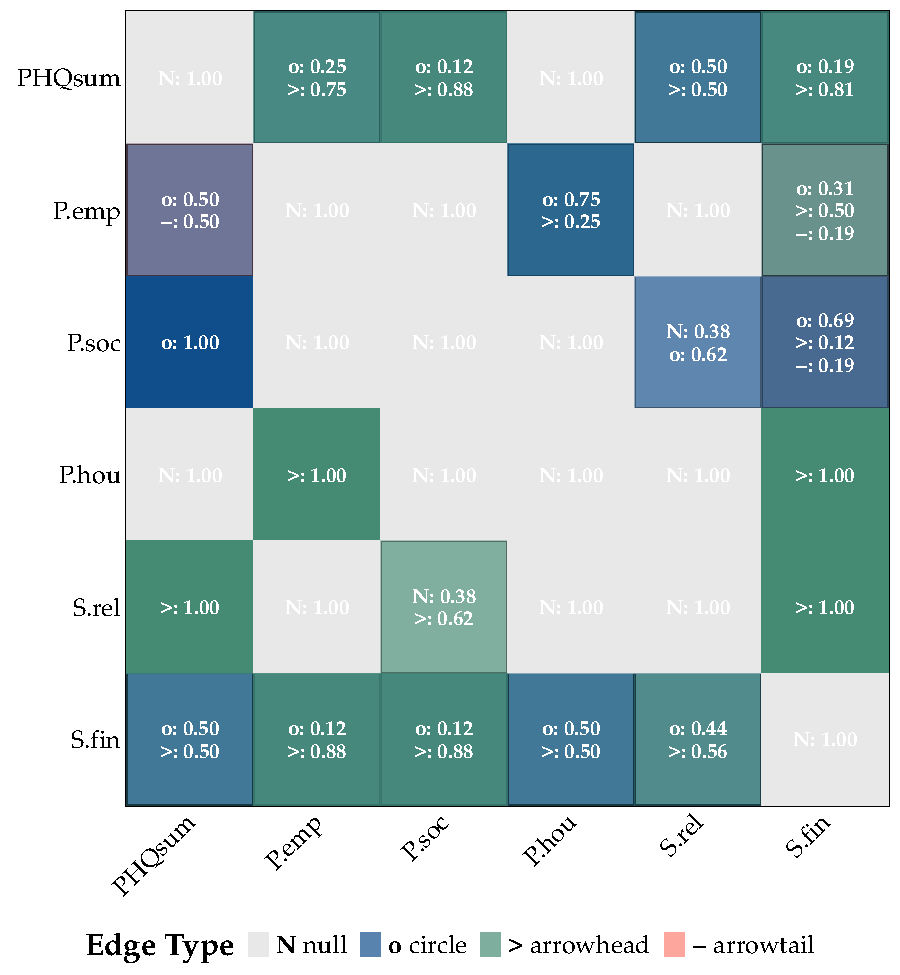
\includegraphics[width=1\textwidth,height=\textheight]{img/depsum_mat_cci.pdf}

}

\subcaption{\label{fig-sum-cci-2}Proportion matrix}

\end{minipage}%

\caption{\label{fig-sum-cci}Resulting graph of precariousness factors
and depression sum score using CCI and proportion of edge endpoint
types.}

\end{figure}%

\begin{figure}

\begin{minipage}{\linewidth}

\centering{

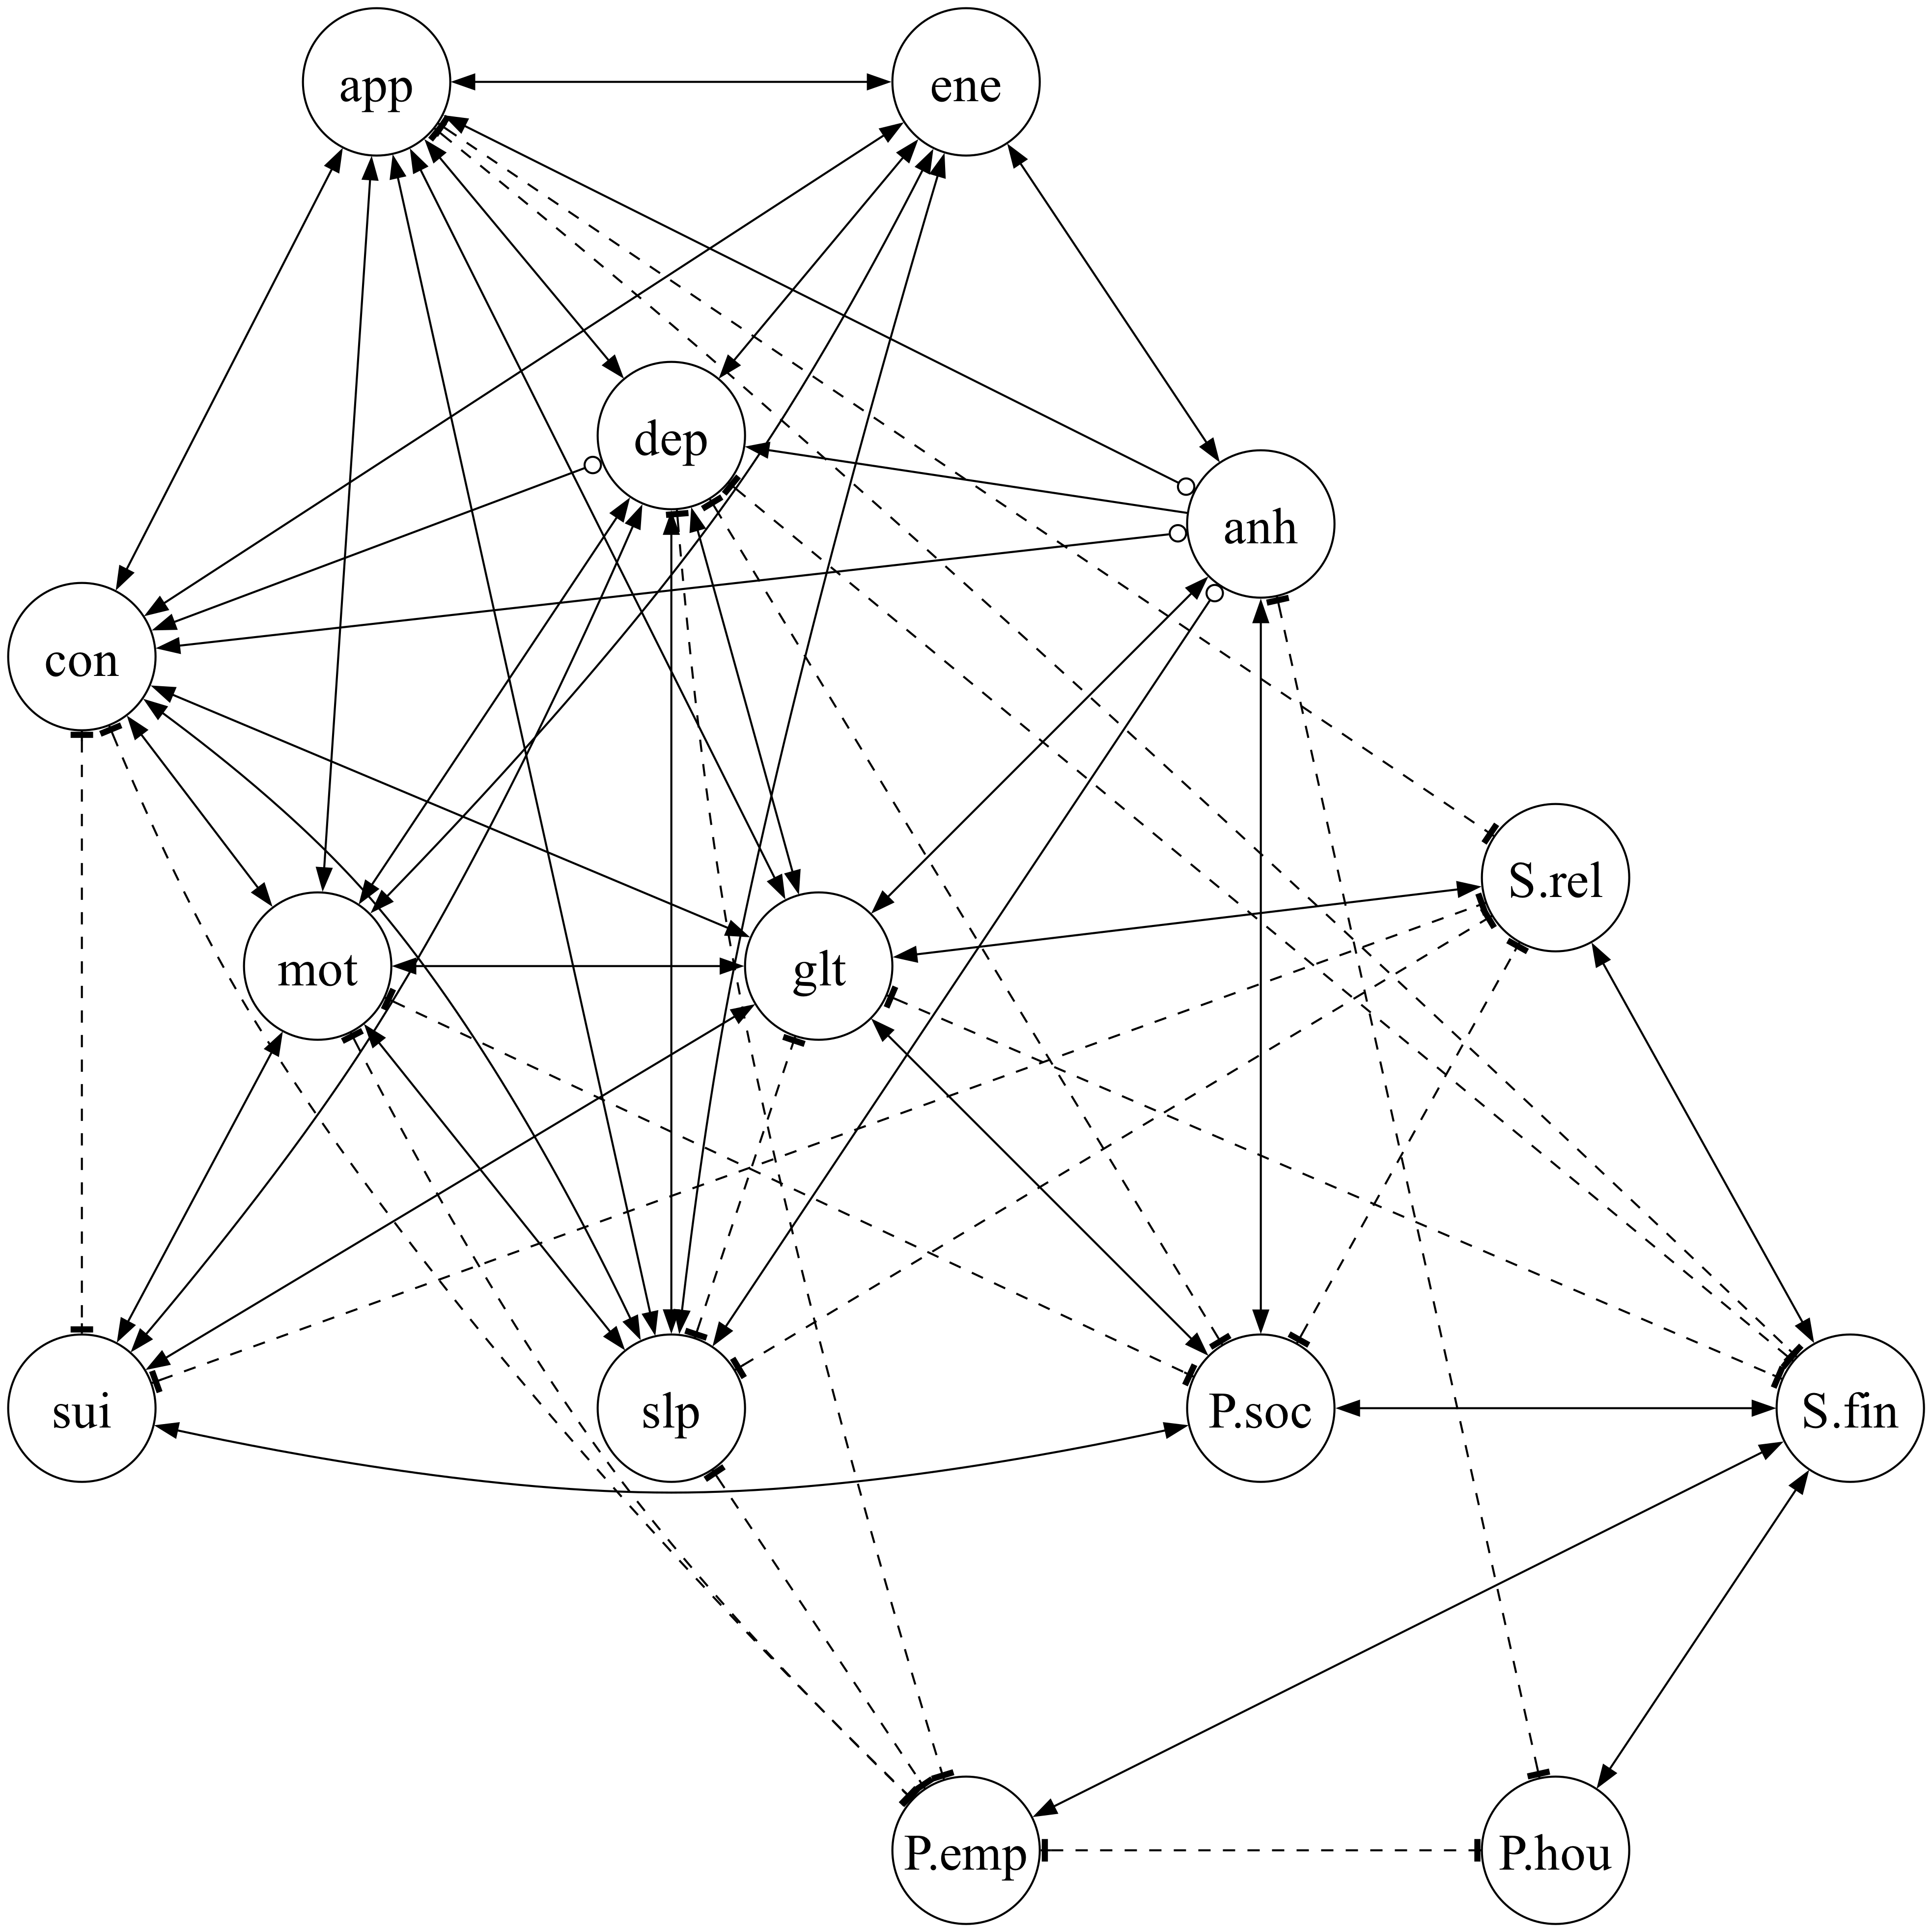
\includegraphics[width=0.6\textwidth,height=\textheight]{img/symptom_graph_CCI.png}

}

\subcaption{\label{fig-sym-cci-1}CCI MAAG}

\end{minipage}%
\newline
\begin{minipage}{\linewidth}

\centering{

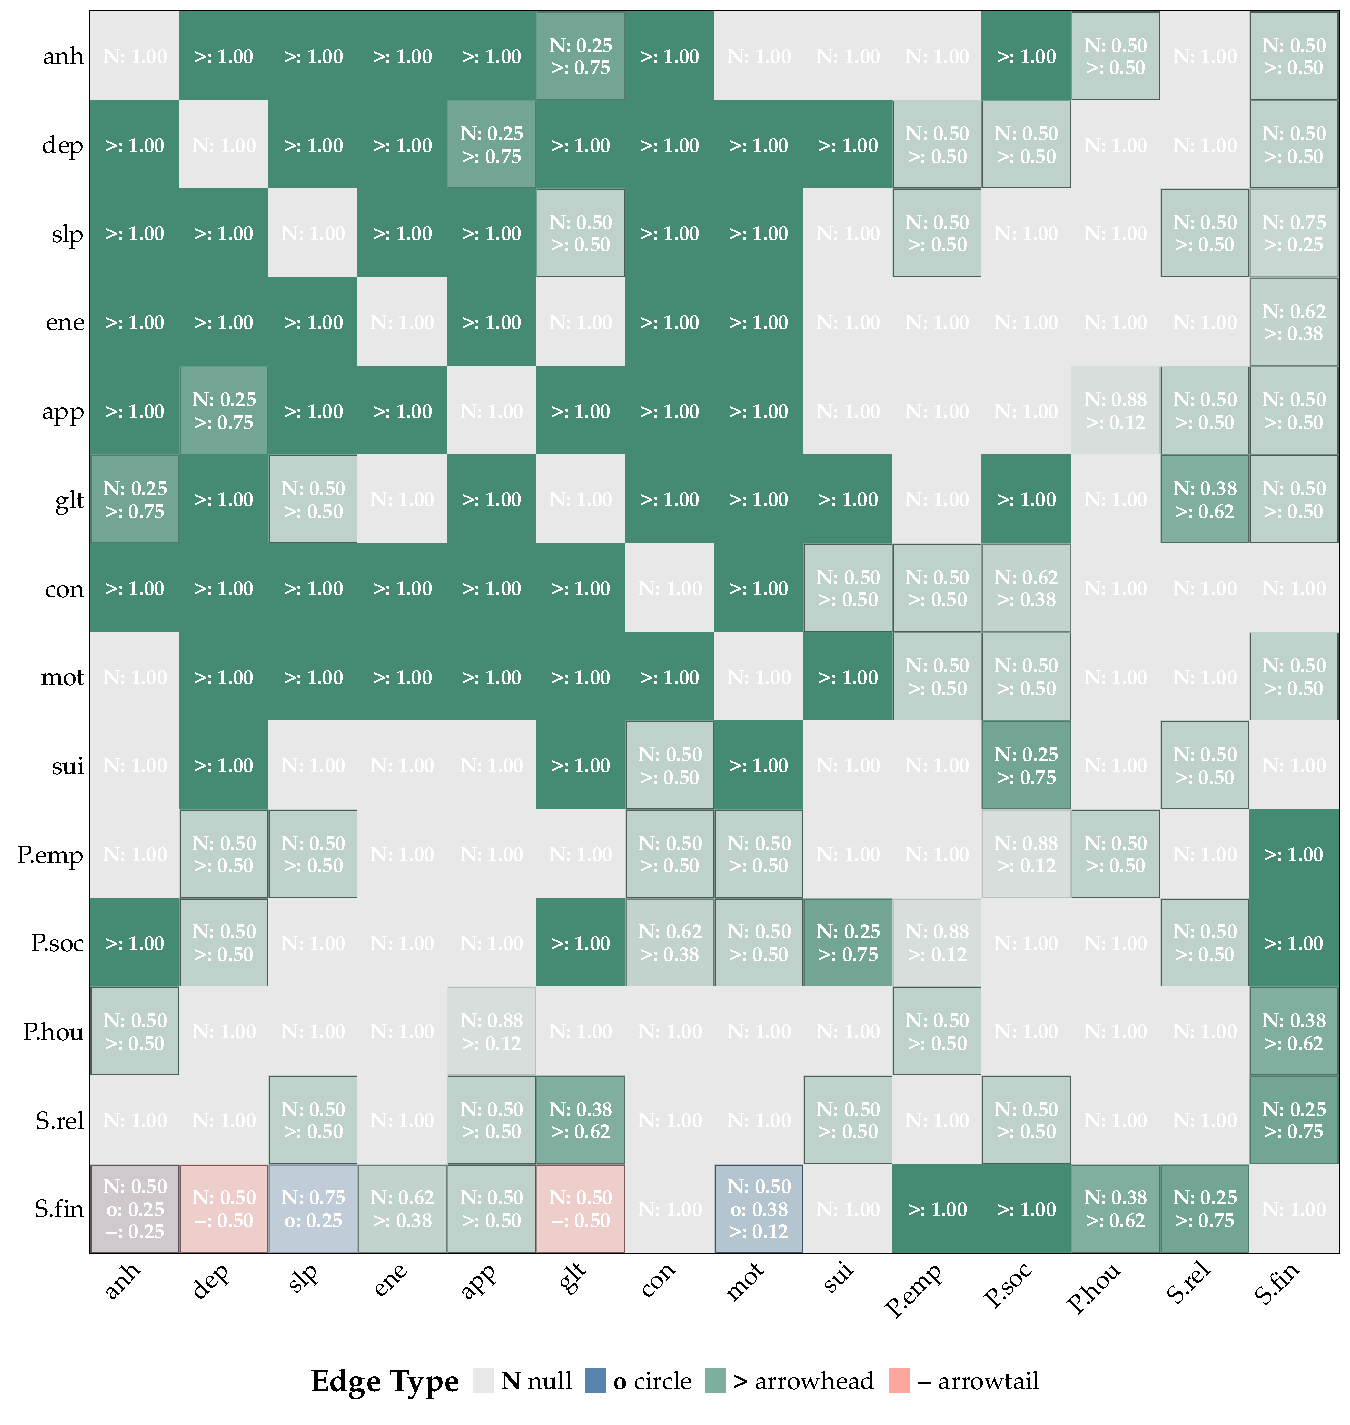
\includegraphics[width=0.6\textwidth,height=\textheight]{img/symptom_mat_cci.pdf}

}

\subcaption{\label{fig-sym-cci-2}Proportion matrix}

\end{minipage}%

\caption{\label{fig-sym-cci}Resulting graph of precariousness factors
and individual depression symptoms using CCI and proportion of edge
endpoint types.}

\end{figure}%

\begin{figure}

\begin{minipage}{\linewidth}

\centering{

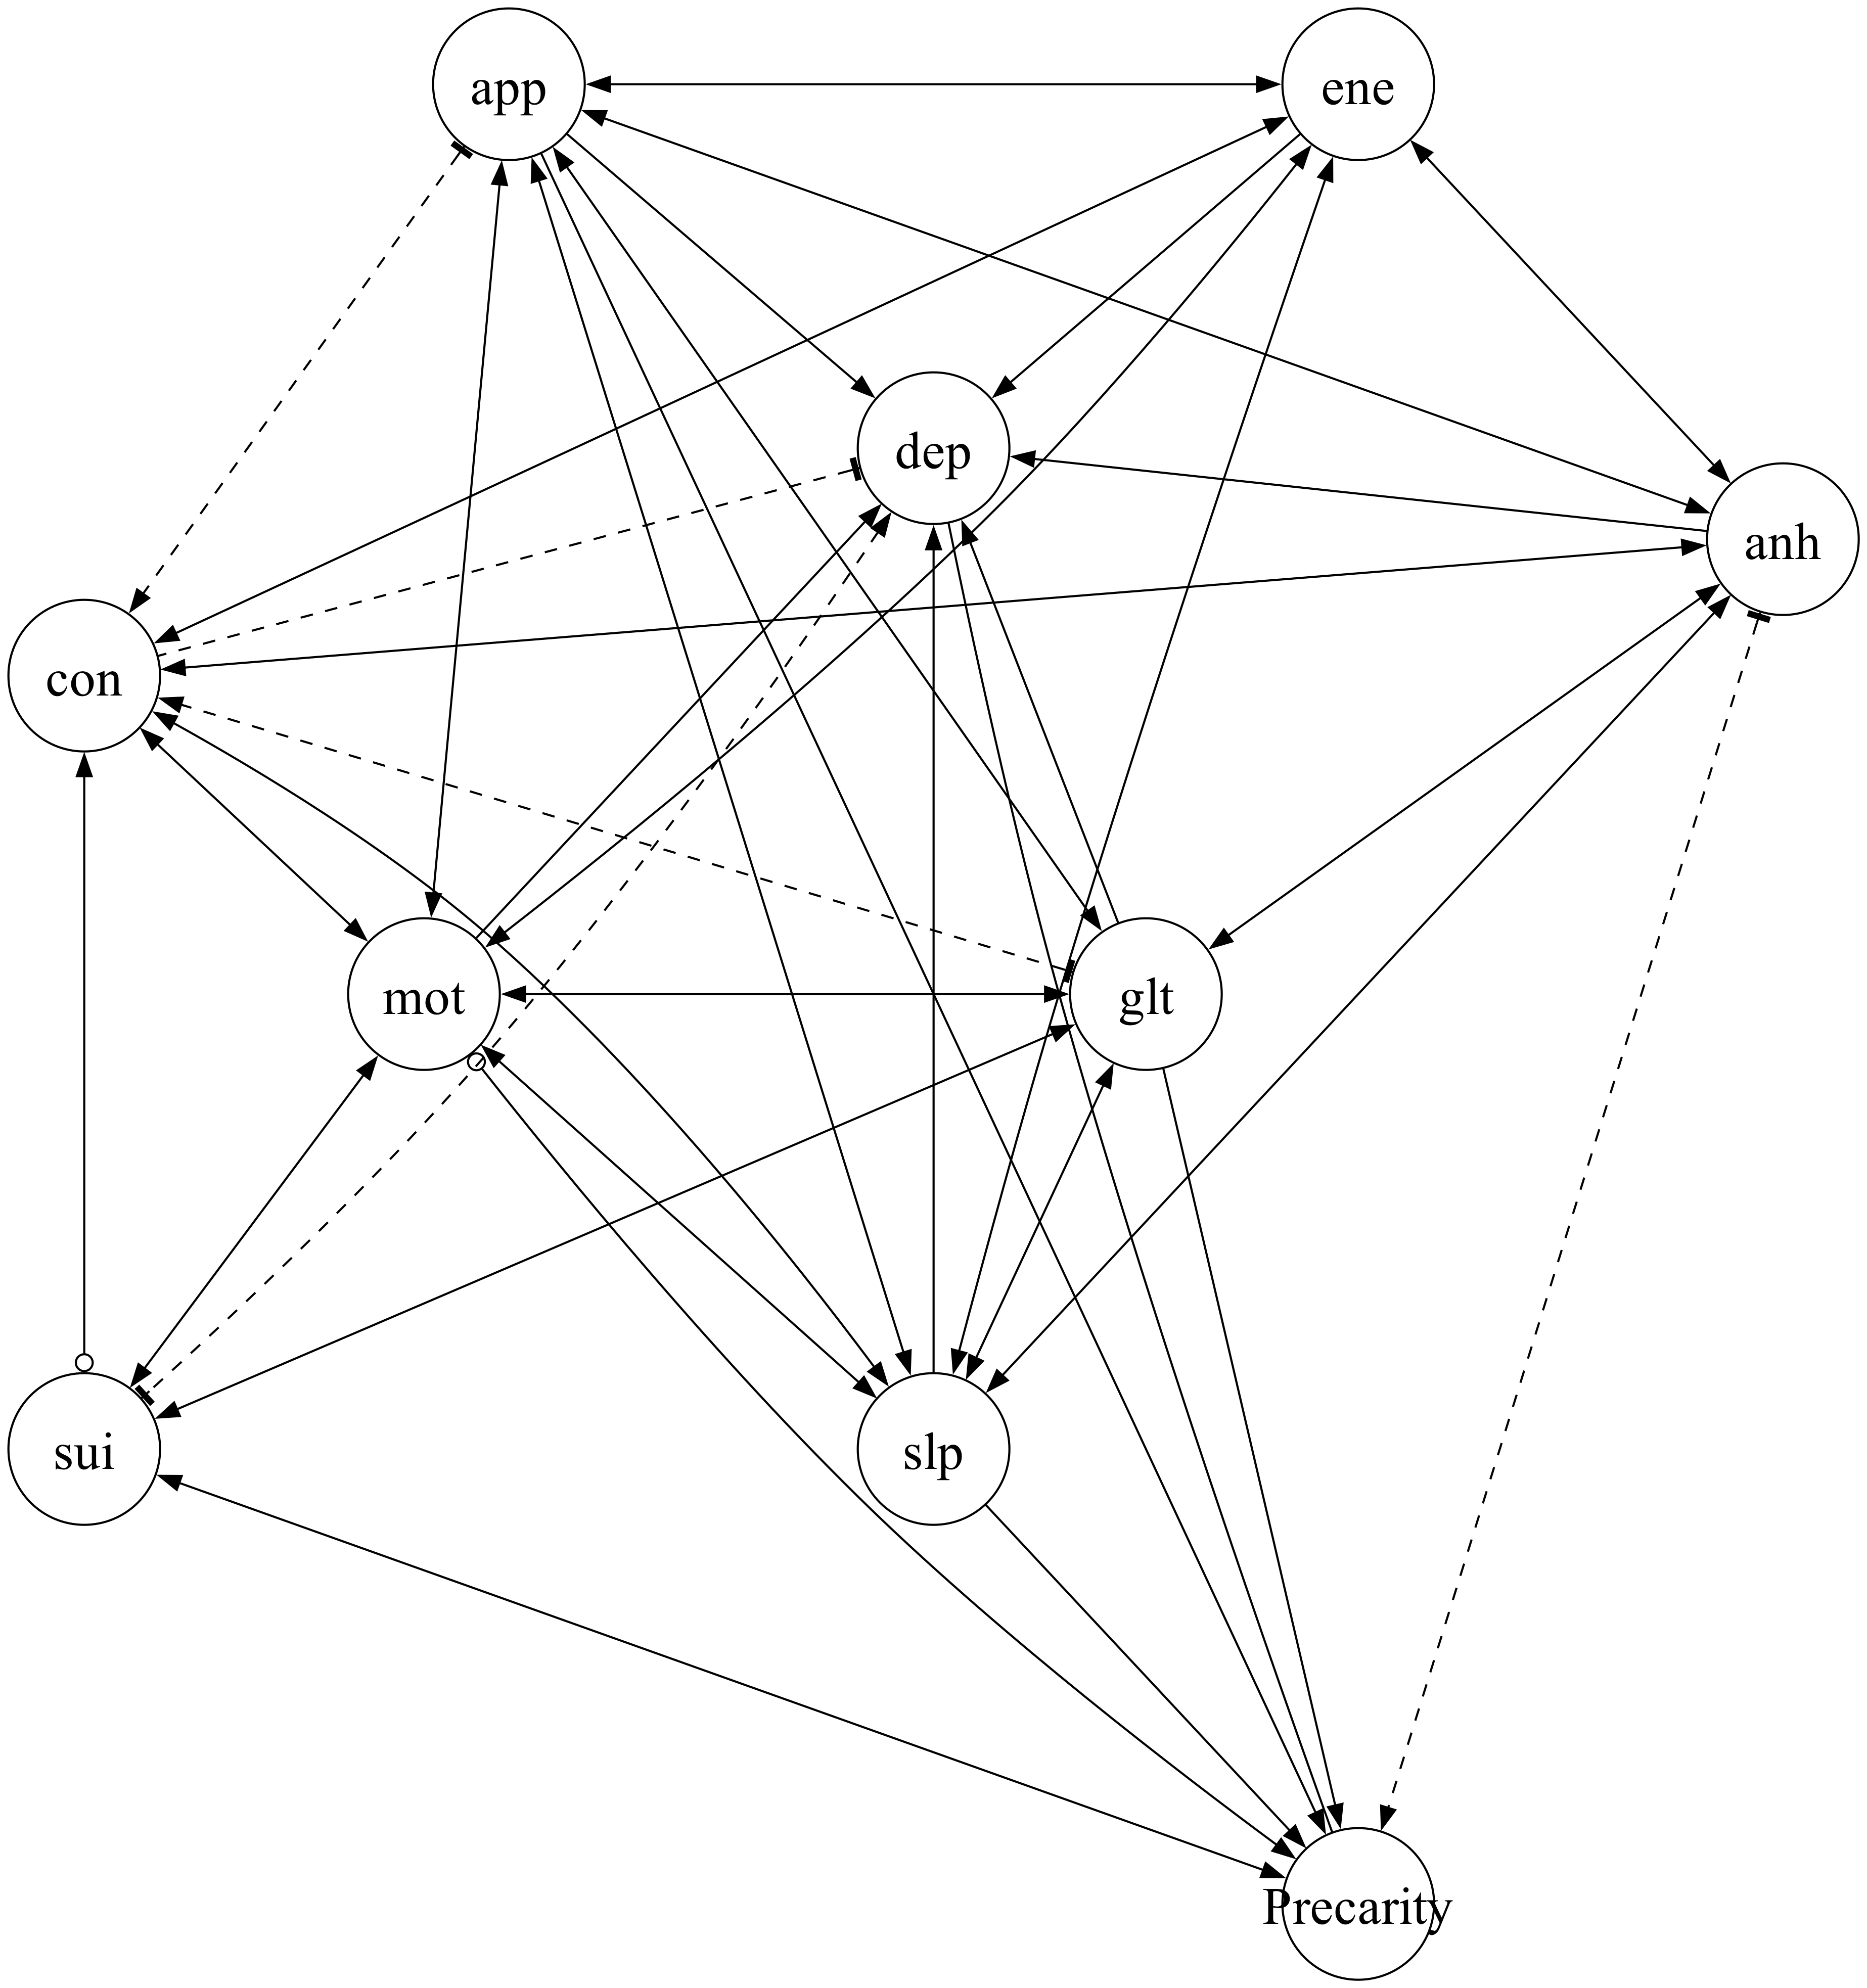
\includegraphics[width=0.6\textwidth,height=\textheight]{img/presum_graph_CCI.png}

}

\subcaption{\label{fig-presum-cci-1}CCI MAAG}

\end{minipage}%
\newline
\begin{minipage}{\linewidth}

\centering{

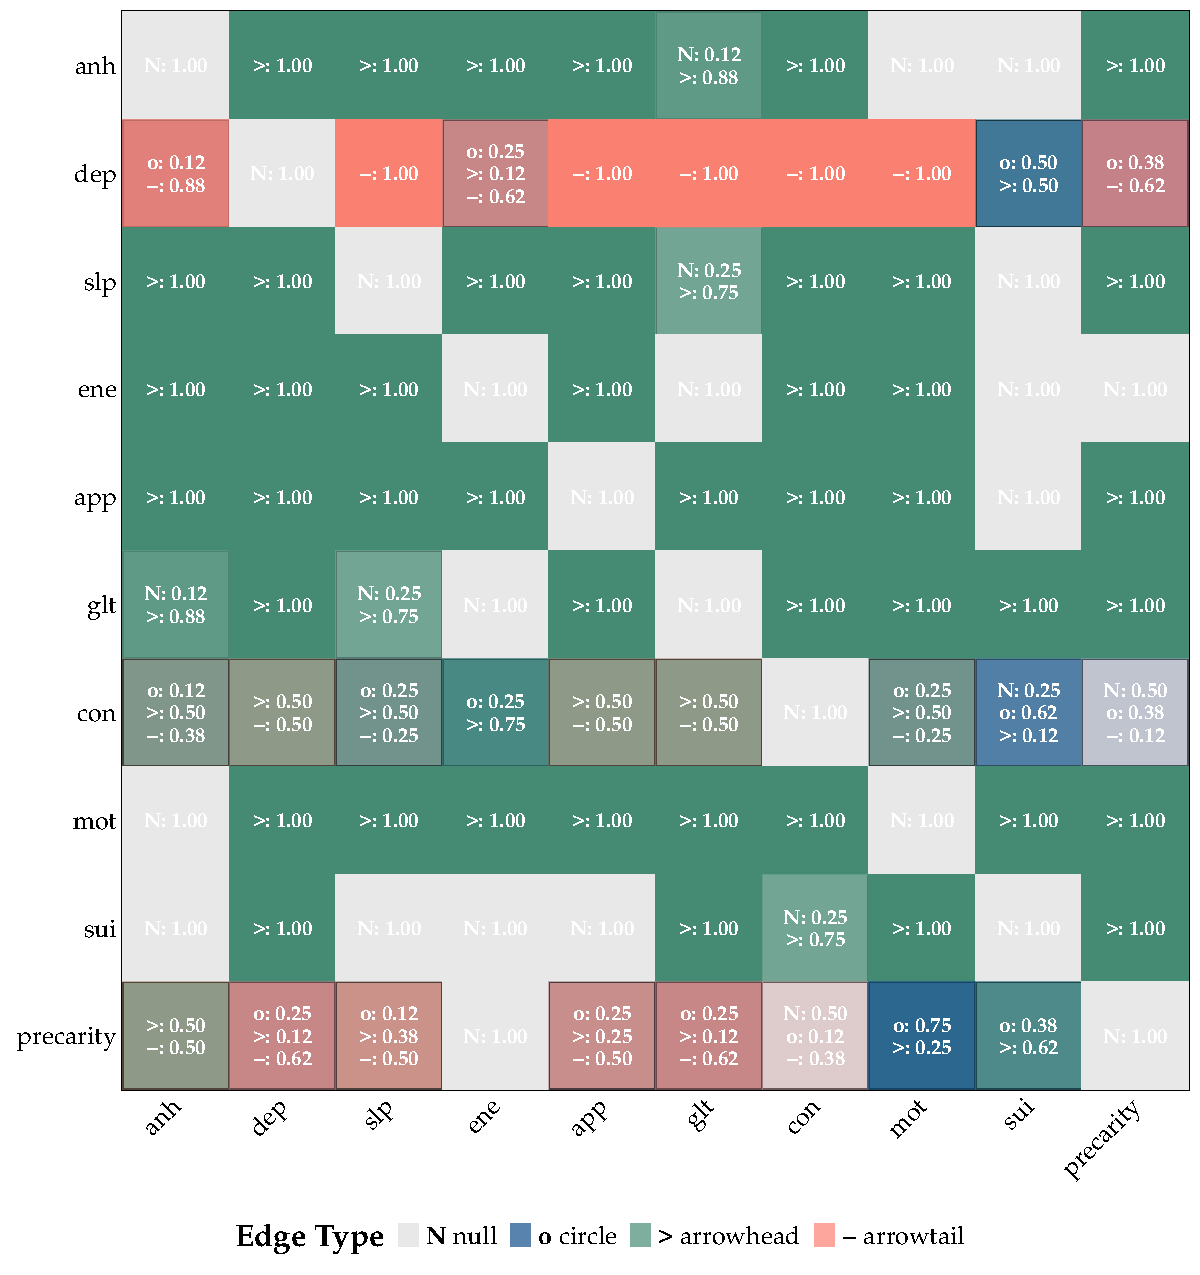
\includegraphics[width=0.6\textwidth,height=\textheight]{img/presum_mat_cci.pdf}

}

\subcaption{\label{fig-presum-cci-2}Proportion matrix}

\end{minipage}%

\caption{\label{fig-presum-cci}Resulting graph of precariousness sum
score and individual depression symptoms using CCI and proportion of
edge endpoint types.}

\end{figure}%

\clearpage

\subsection{Results from PC algorithm}\label{sec-pc}

\begin{figure}

\begin{minipage}{0.50\linewidth}

\centering{

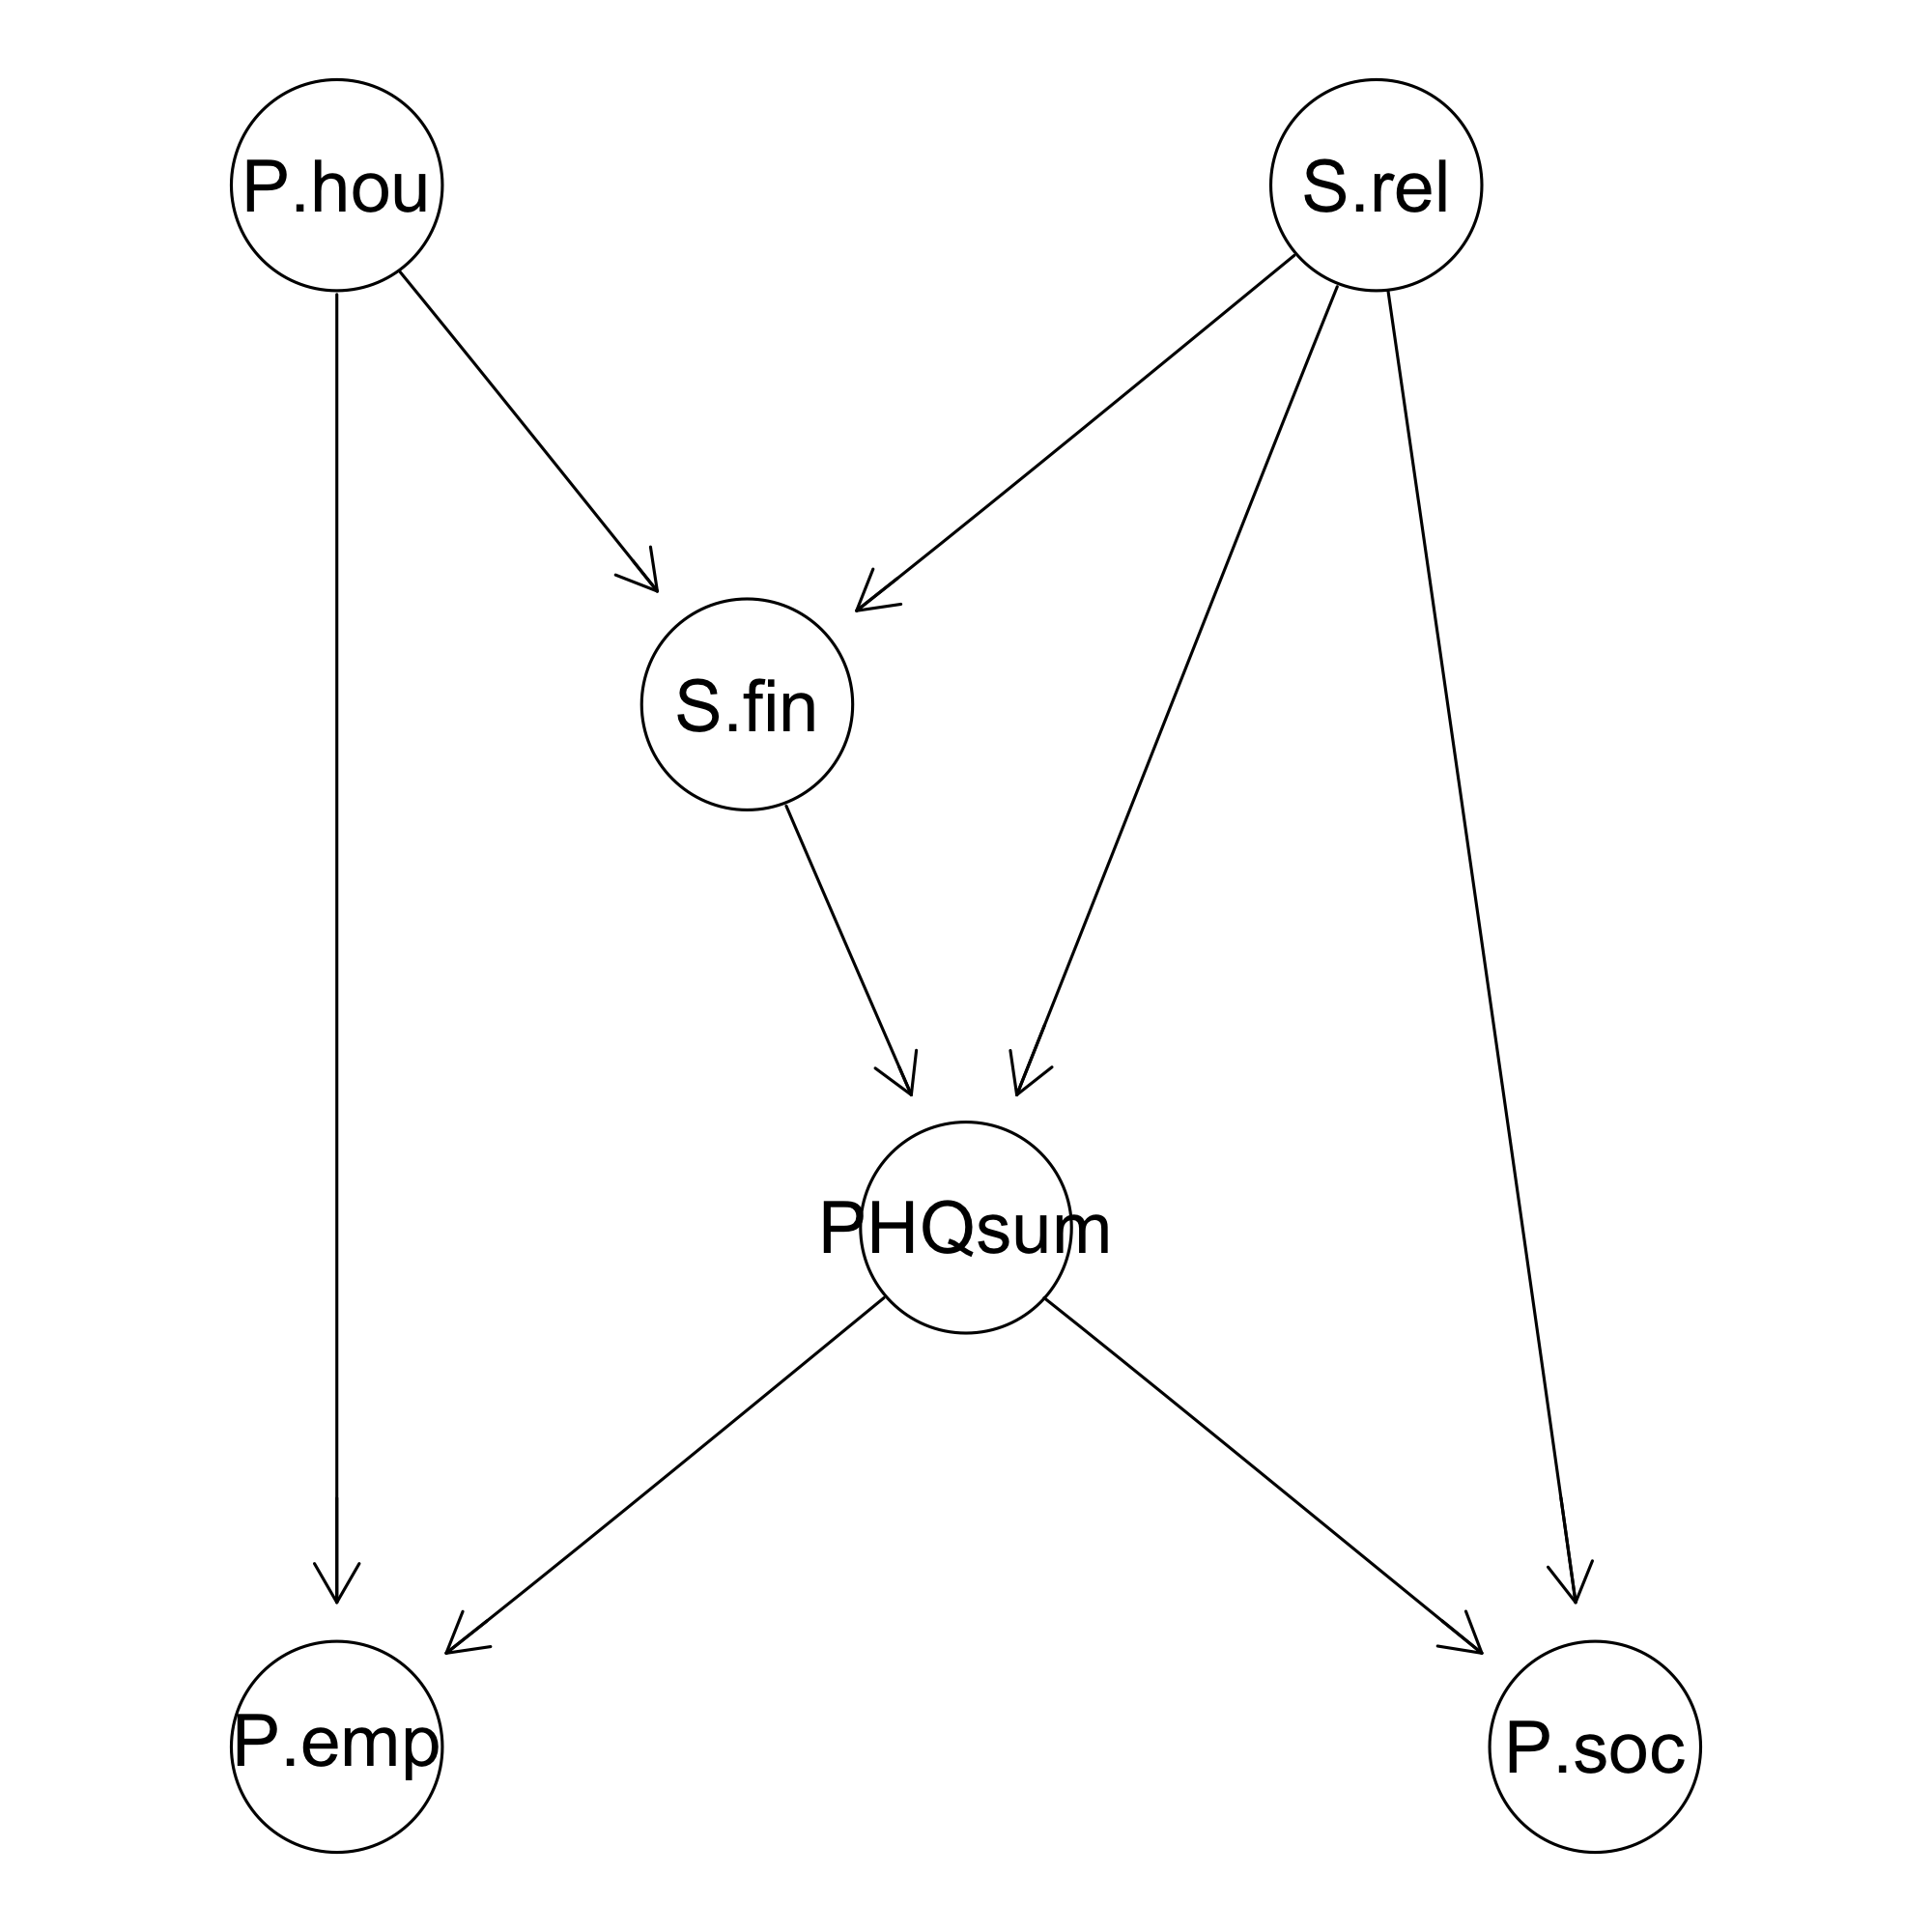
\includegraphics[width=1\textwidth,height=\textheight]{img/sum_PC_all.png}

}

\subcaption{\label{fig-pc_sum-1}Using both GaussianCI and RCoT}

\end{minipage}%
%
\begin{minipage}{0.50\linewidth}

\centering{

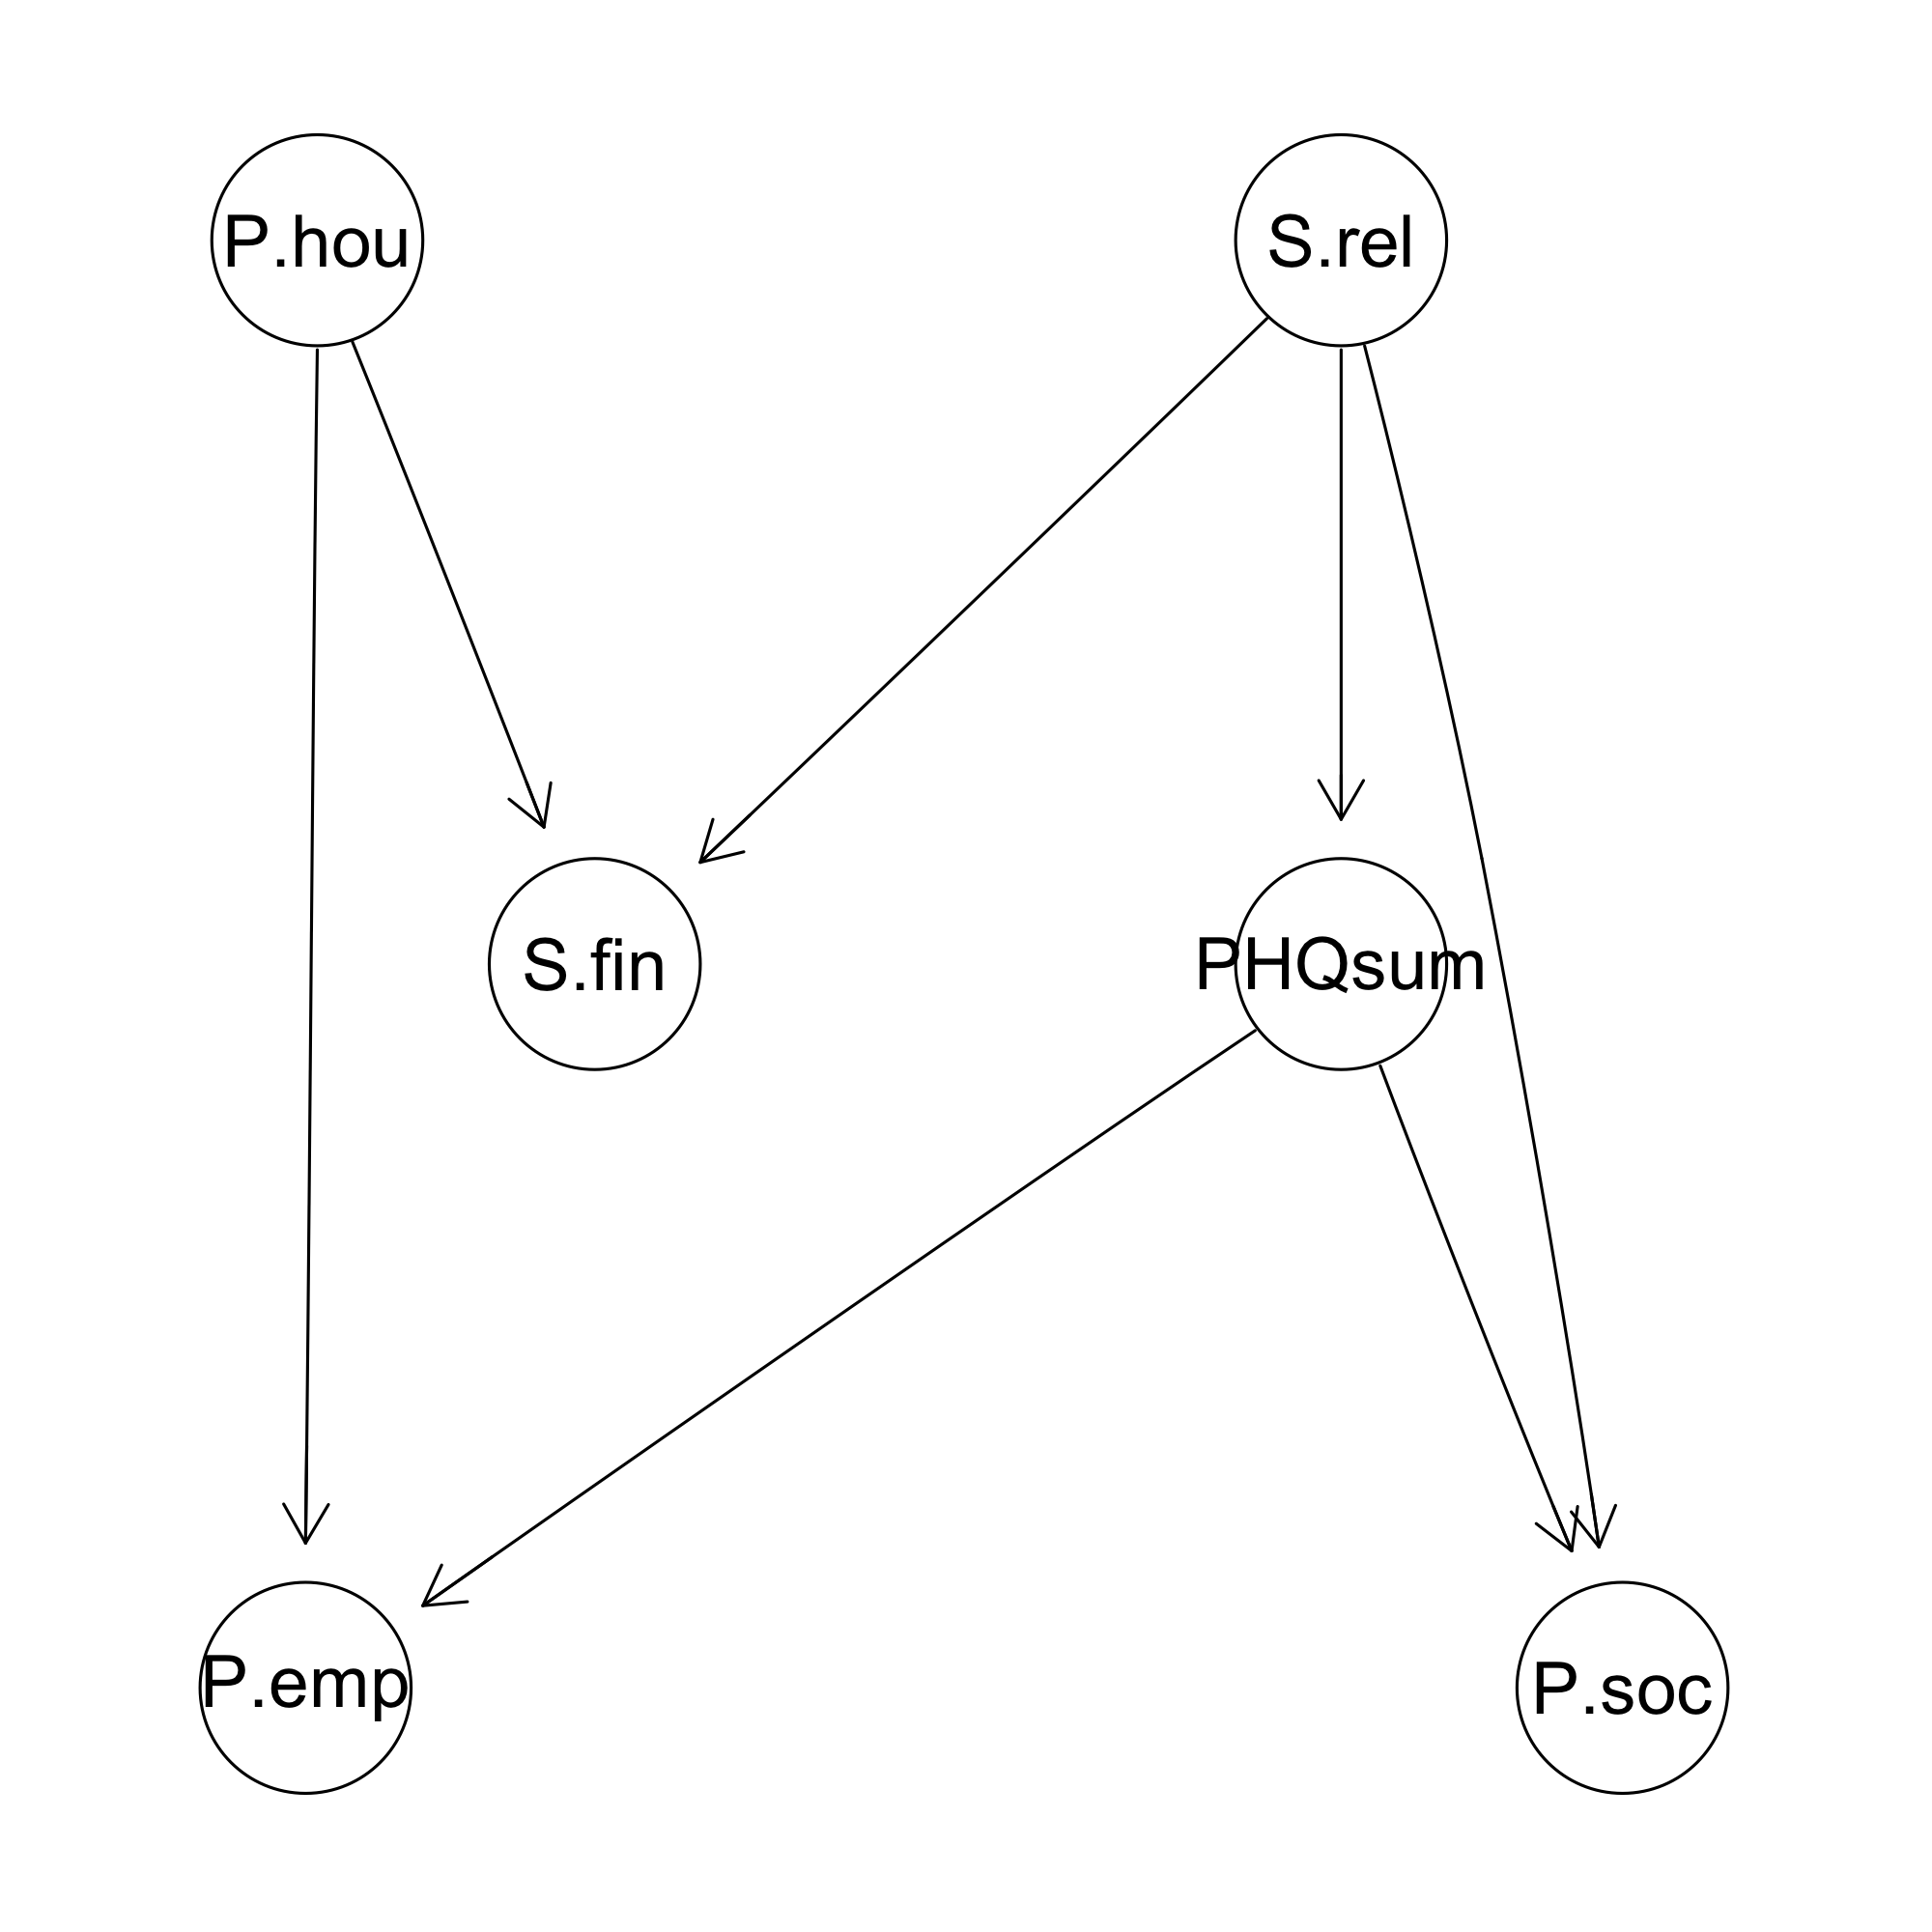
\includegraphics[width=1\textwidth,height=\textheight]{img/sum_PC_RCoTonly.png}

}

\subcaption{\label{fig-pc_sum-2}Using only RCoT}

\end{minipage}%

\caption{\label{fig-pc_sum}Resulting graphs of precariousness factors
and depression sum score using PC.}

\end{figure}%

\begin{figure}

\centering{

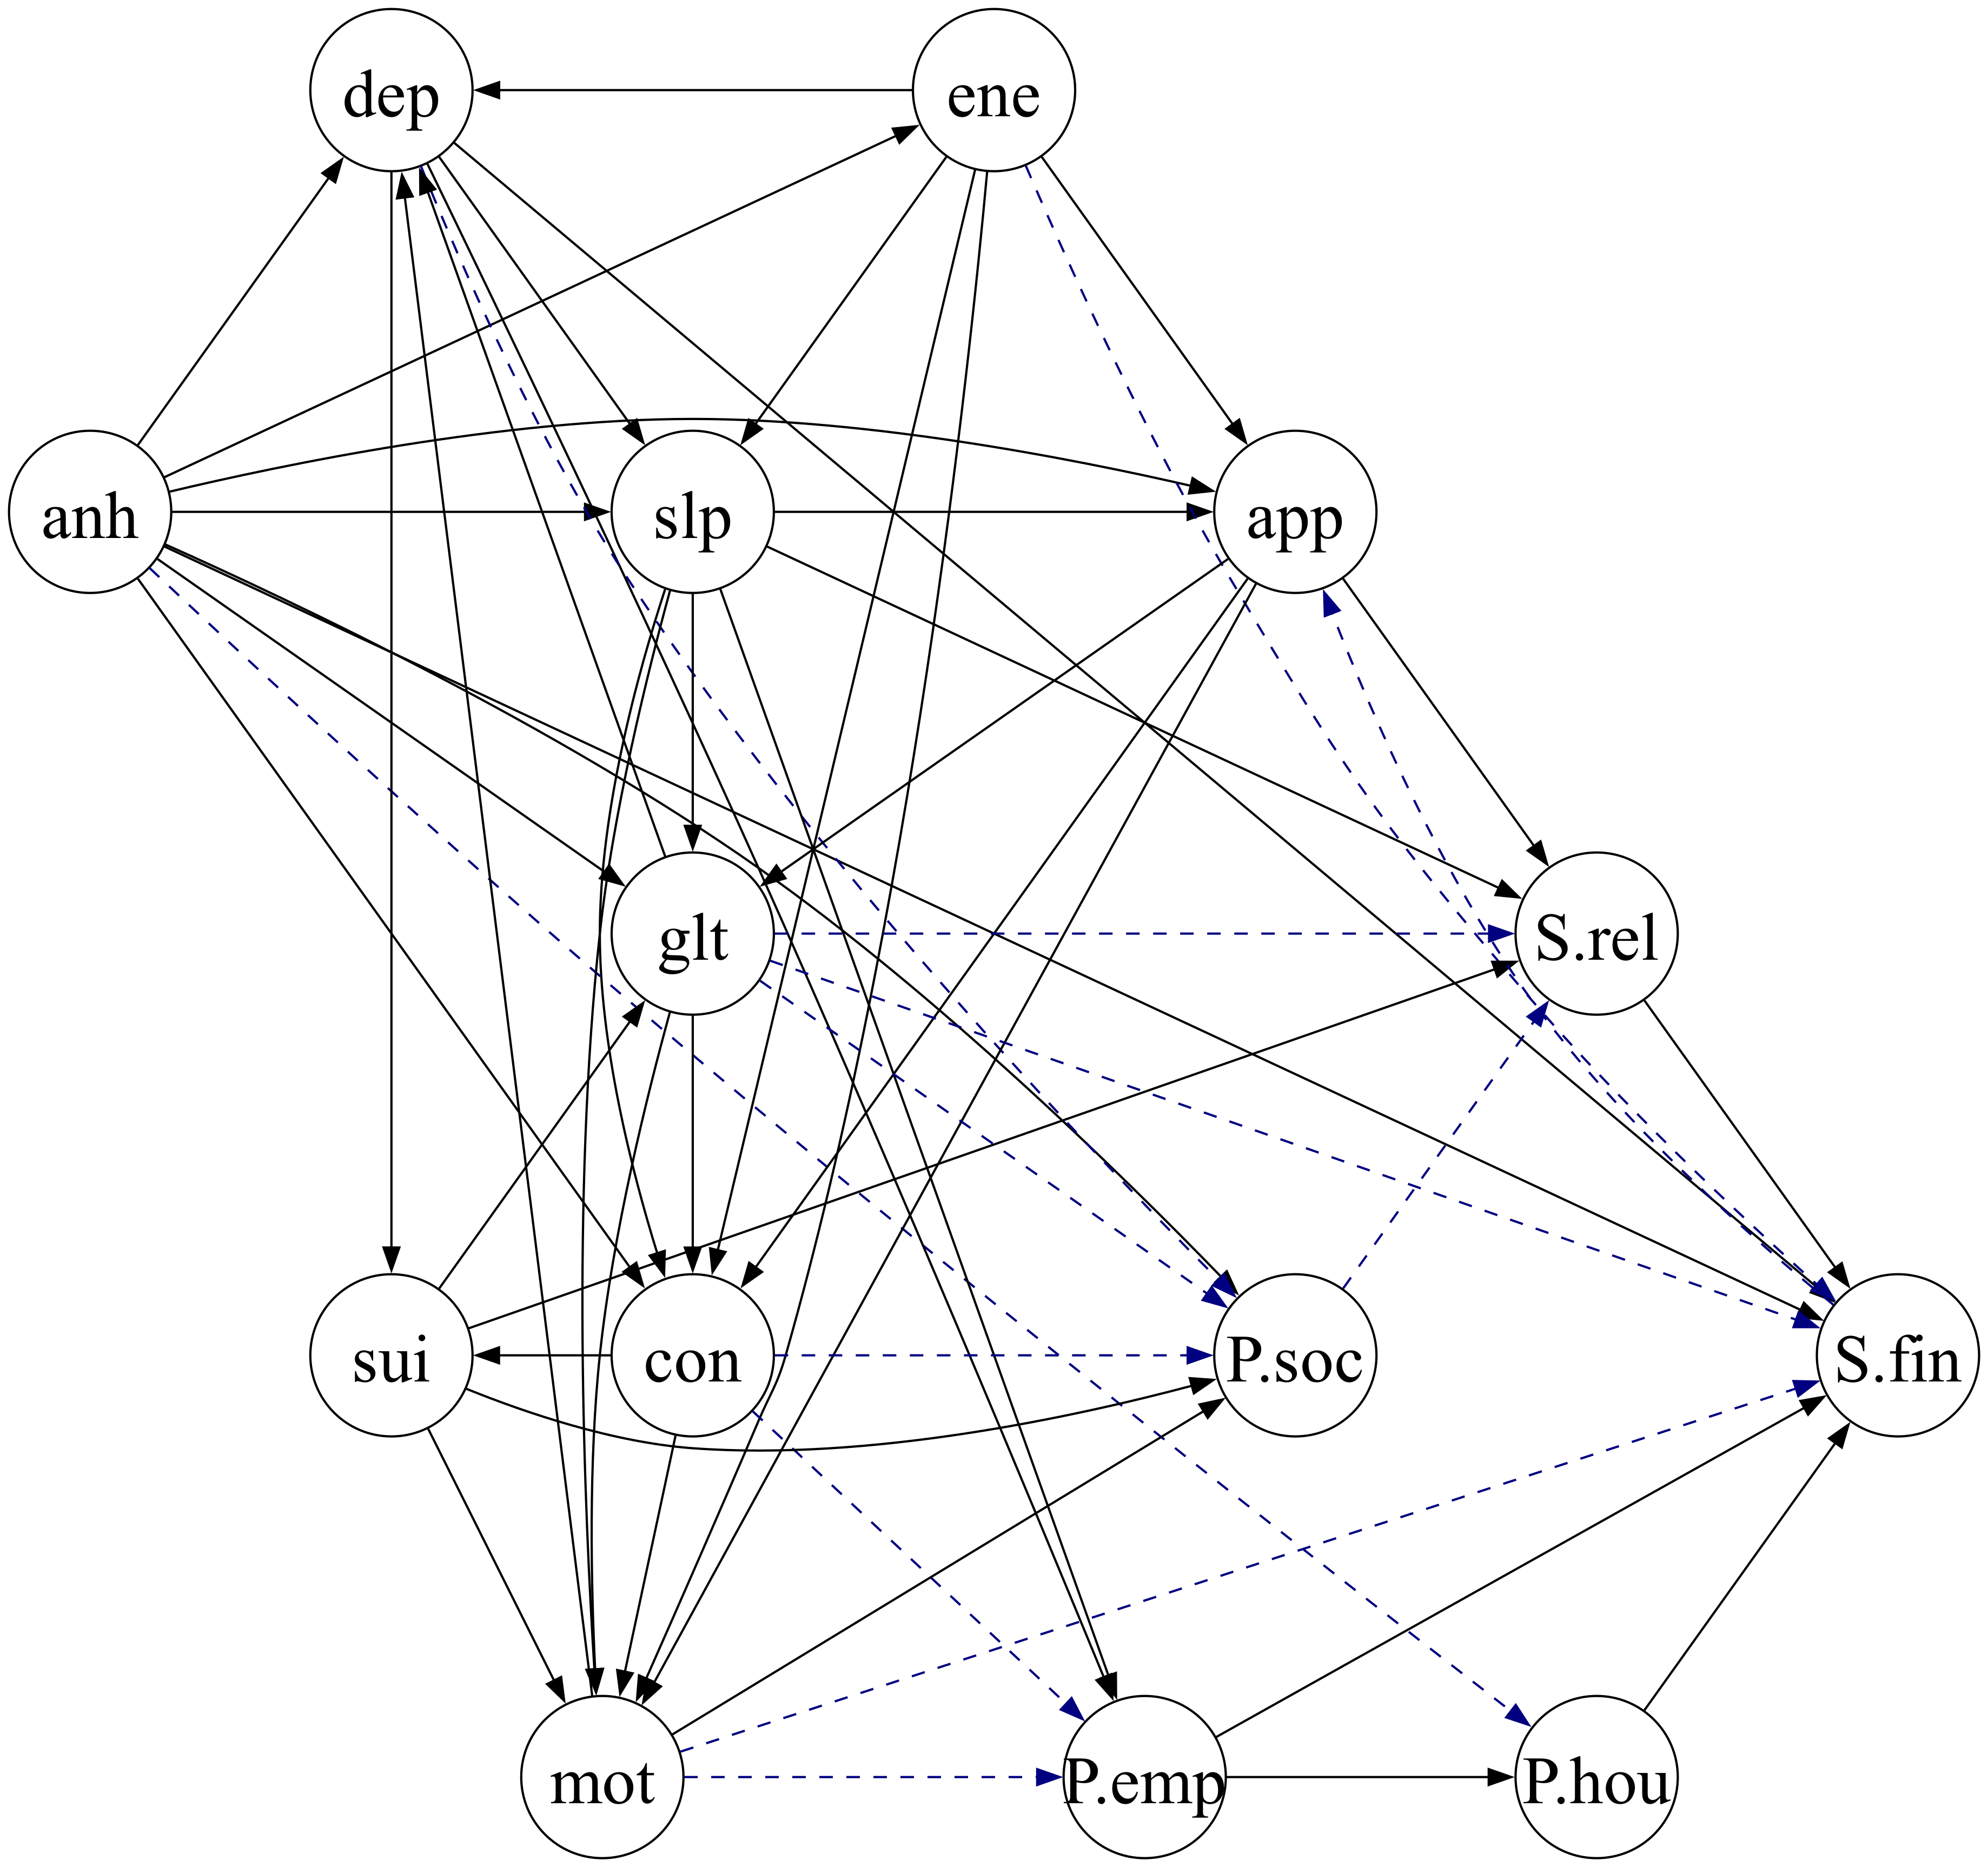
\includegraphics[width=0.6\textwidth,height=\textheight]{img/PC_symptom.png}

}

\caption{\label{fig-pc_sym}Resulting graphs of precariousness factors
and individual depression symptoms using PC.}

\end{figure}%

\begin{figure}

\centering{

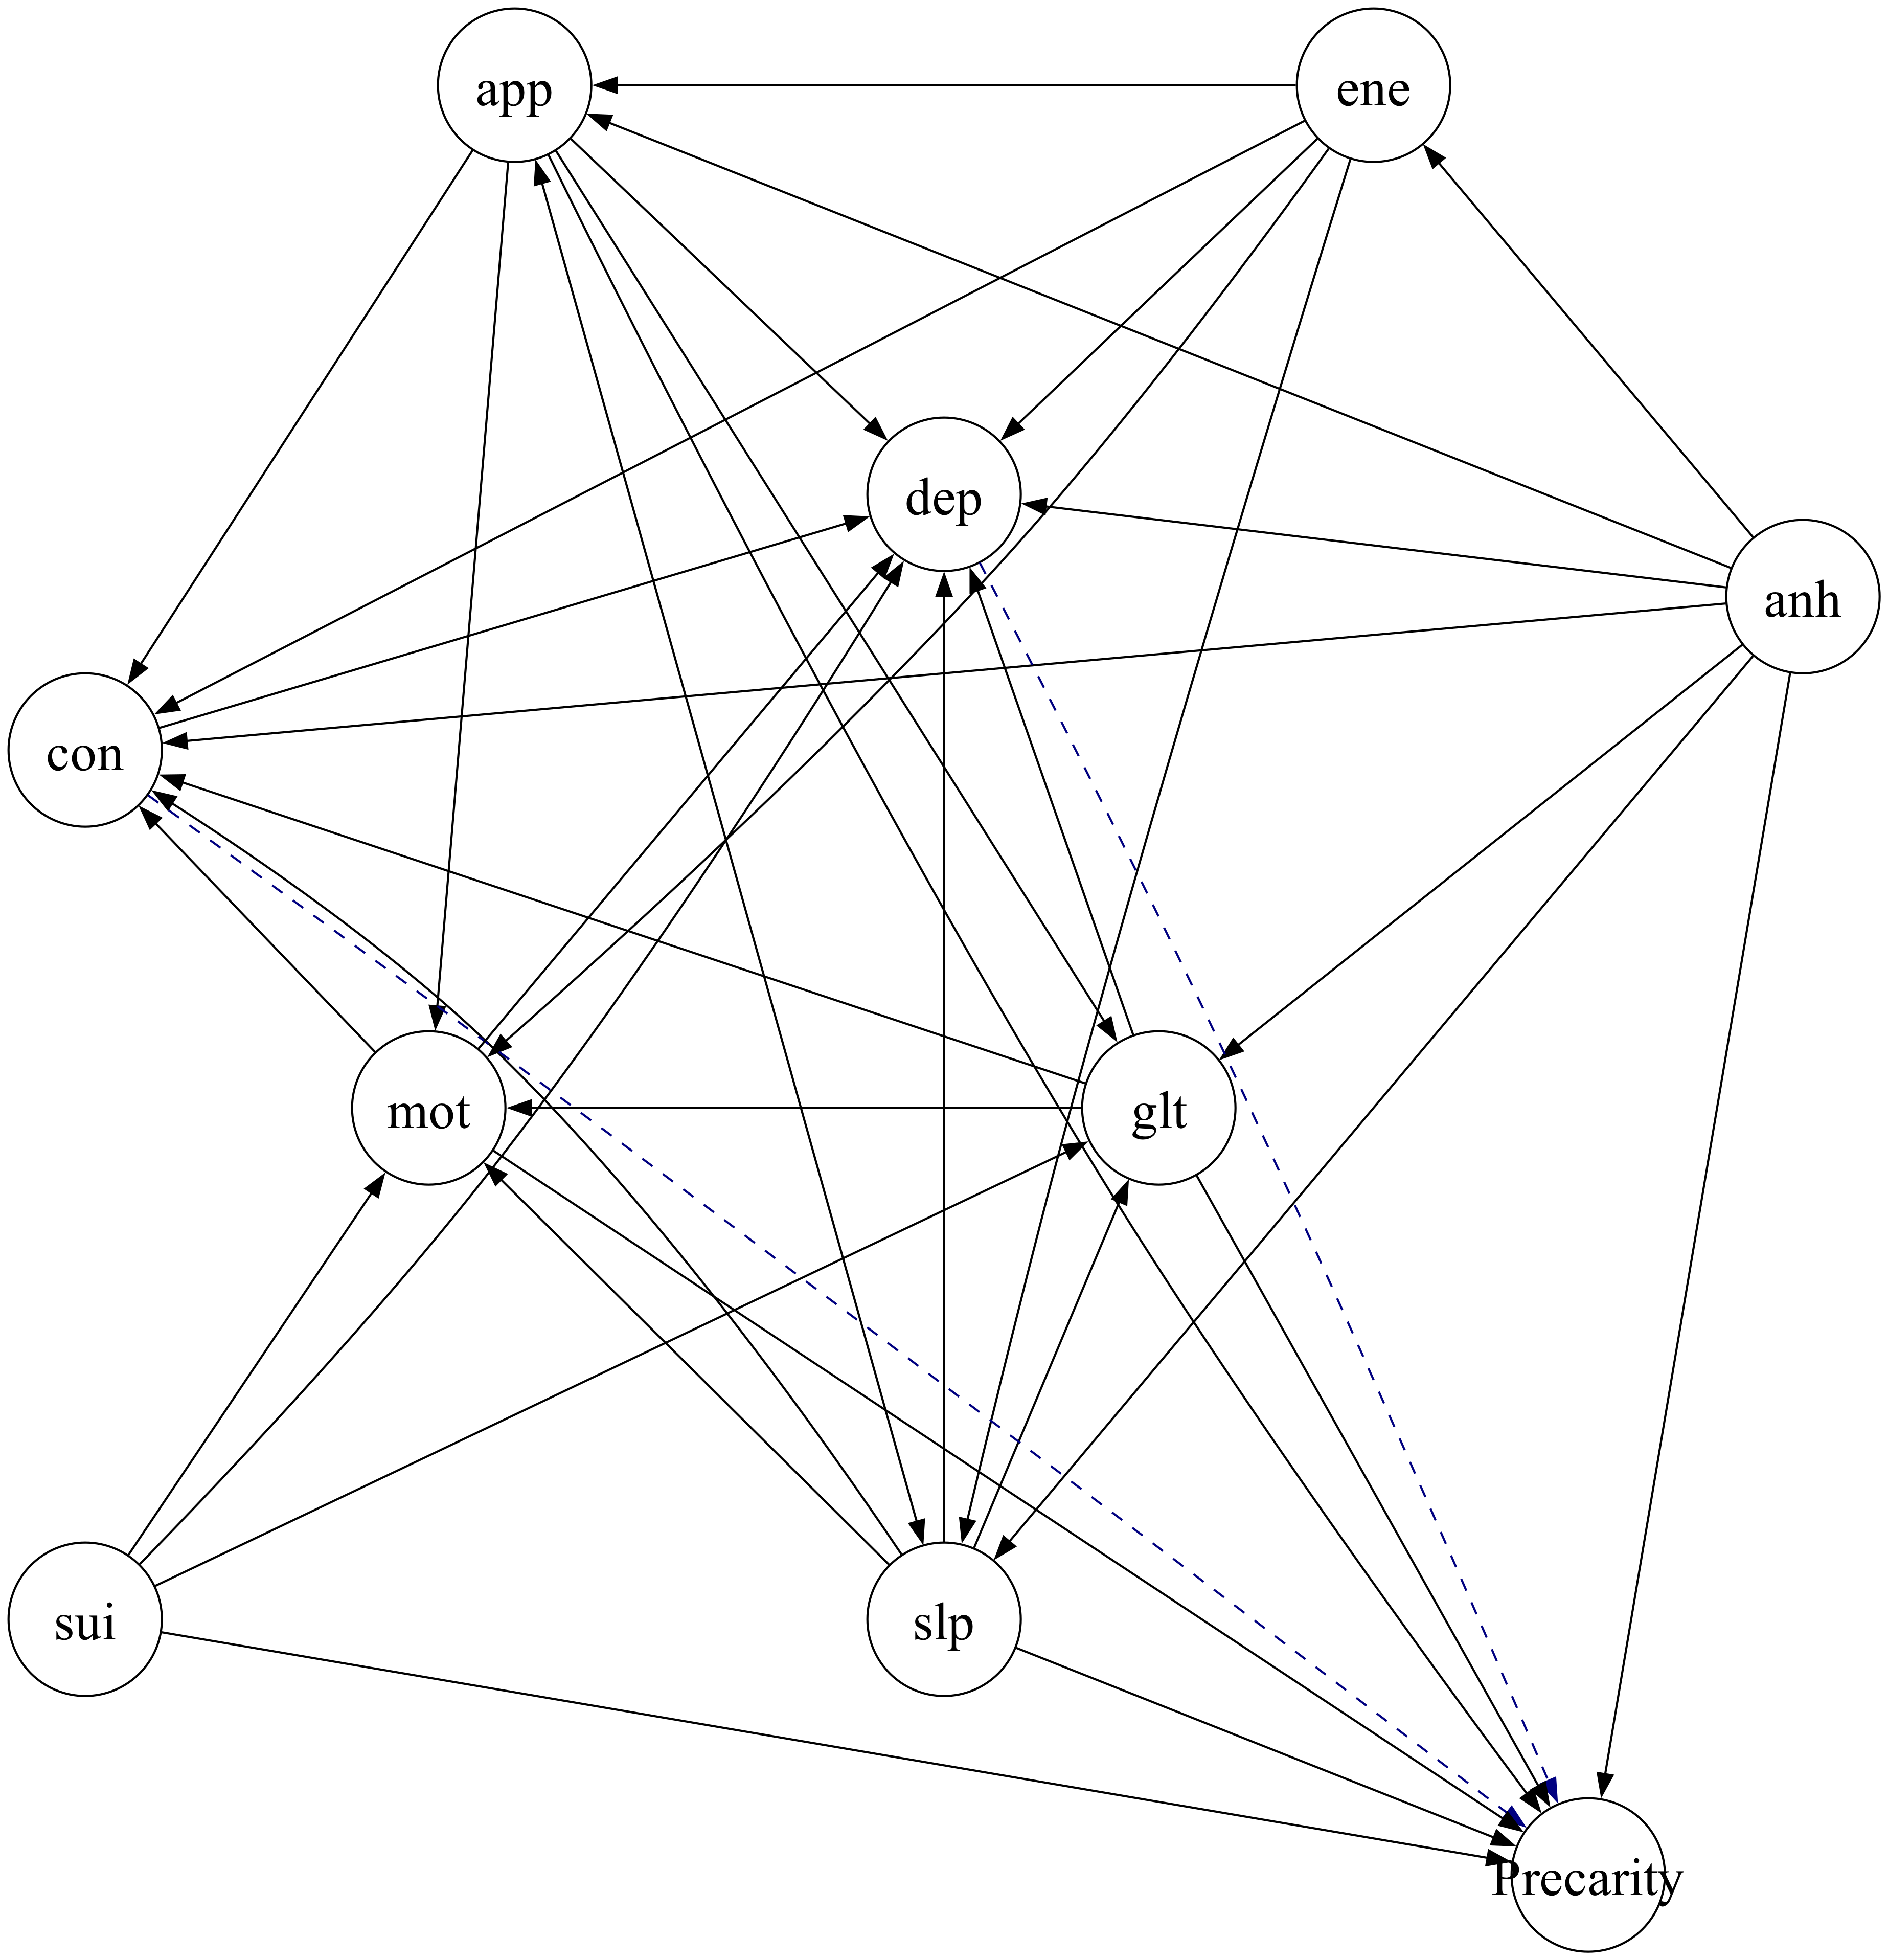
\includegraphics[width=0.6\textwidth,height=\textheight]{img/PC_presum.png}

}

\caption{\label{fig-pc_presum}Resulting graphs of precariousness sum
score and individual depression symptoms using PC.}

\end{figure}%

\clearpage

\subsection{Randomized Conditional Independence / Correlation Test (RCIT
\& RCoT)}\label{sec-rcot}

RCIT (Randomized Conditional Independence Test) and RCoT (Randomized
conditional Correlation Test) are advanced methods for scalable
conditional independence (CI) testing, offering computational efficiency
while maintaining the accuracy of kernel-based approaches. These methods
evaluate conditional independence between two variables \(X\) and \(Y\)
given a third variable \(Z\) while addressing computational challenges
inherent in kernel-based CI tests. In this section, we provide a
high-level overview of RCIT and RCoT based on (Strobl et al., 2019).

\subsubsection{Kernel-Based Conditional Independence
Testing}\label{kernel-based-conditional-independence-testing}

Traditional kernel-based CI tests, such as the Kernel Conditional
Independence Test (KCIT), compute dependencies using the Hilbert-Schmidt
Independence Criterion (HSIC) in reproducing kernel Hilbert spaces
(RKHS) (Zhang et al., 2012). KCIT uses the following hypothesis
framework: \[
H_0: X \perp\!\!\!\perp Y \,|\, Z, \quad H_1: X \not\!\perp\!\!\!\perp Y \,|\, Z.
\] The core quantity in KCIT is the partial cross-covariance operator:
\[
\Sigma_{XY \cdot Z} = \Sigma_{XY} - \Sigma_{XZ} \Sigma_{ZZ}^{-1} \Sigma_{ZY},
\] where \(\Sigma_{XY}\) represents the cross-covariance operator
between \(X\) and \(Y\), and
\(\Sigma_{XZ} \Sigma_{ZZ}^{-1} \Sigma_{ZY}\) removes the dependence
mediated by \(Z\).

The squared Hilbert-Schmidt (HS) norm of \(\Sigma_{XY \cdot Z}\) serves
as the test statistic: \[
\|\Sigma_{XY \cdot Z}\|^2_{HS} = 0 \quad \text{if and only if} \quad X \perp\!\!\!\perp Y \,|\, Z.
\]

KCIT estimates residual dependencies using kernel ridge regression: \[
f^*(z) = K_Z (K_Z + \lambda I)^{-1} f(x),
\] where \(K_Z\) is the kernel matrix for \(Z\), \(f(x)\) is the kernel
feature map for \(X\), and \(\lambda\) is the ridge regularization
parameter. The residual function for \(X\) is: \[
f_\text{res}(x) = f(x) - f^*(z) = R_Z f(x),
\] with: \[
R_Z = I - K_Z (K_Z + \lambda I)^{-1}.
\] The kernel matrix for residualized \(X\) is: \[
K_{X \cdot Z} = R_Z K_X R_Z,
\] and similarly for \(Y\), \(K_{Y \cdot Z} = R_Z K_Y R_Z\).

The test statistic is computed as: \[
T_{XY \cdot Z} = \frac{1}{n^2} \text{tr}(K_{X \cdot Z} K_{Y \cdot Z}),
\] which estimates the Hilbert-Schmidt (HS) norm of the partial
cross-covariance operator. To ensure convergence, KCIT scales the
statistic by \(n\): \[
S_K = n T_{XY \cdot Z}.
\] The null hypothesis \(H_0\) is rejected if \(S_K\) exceeds a
threshold determined by permutation or moment-matching-based null
distribution (Lindsay et al., 2000).

\subsubsection{Random Fourier Features
(RFFs)}\label{random-fourier-features-rffs}

Kernel-based methods like KCIT face scalability issues, as they involve
operations on \(n \times n\) kernel matrices, which scale quadratically
with the sample size \(n\). RCIT and RCoT overcome this bottleneck using
\emph{Random Fourier Features (RFFs)} to approximate kernel operations
efficiently.

\paragraph{Bochner's Theorem}\label{bochners-theorem}

Bochner's theorem provides the foundation for RFFs, stating that any
continuous shift-invariant kernel \(k(x, y)\) can be expressed as: \[
k(x, y) = \int_{\mathbb{R}^p} e^{i \omega^\top (x - y)} \, dP_\omega,
\] where \(P_\omega\) is the spectral distribution of the kernel. For
the widely used RBF kernel: \[
k(x, y) = \exp\left(-\frac{\|x - y\|^2}{2\sigma^2}\right),
\] \(P_\omega\) follows a Gaussian distribution:
\(\omega \sim \mathcal{N}(0, \sigma^2 I)\).

\paragraph{RFF Approximation}\label{rff-approximation}

Using Monte Carlo sampling, the kernel function is approximated as: \[
k(x, y) \approx \phi(x)^\top \phi(y),
\] where \(\phi(x)\) is the random Fourier feature mapping: \[
\phi(x) = \sqrt{\frac{2}{D}} \cos(W^\top x + b),
\] with \(W \sim \mathcal{N}(0, \sigma^2 I)\) and
\(b \sim \text{Uniform}(0, 2\pi)\). Here, \(D\) is the number of Fourier
features, which balances computational efficiency and approximation
accuracy.

\subsubsection{Differences Between RCIT and
RCoT}\label{differences-between-rcit-and-rcot}

RCIT and RCoT differ in their test statistics, computational efficiency,
and practical performance, which makes them suited for different
scenarios in causal discovery. RCIT evaluates the Hilbert-Schmidt norm
of the full partial cross-covariance operator, providing a general test
for conditional independence but at a higher computational cost. RCoT
simplifies the process by using the Frobenius norm of a
finite-dimensional residualized cross-covariance matrix, significantly
reducing complexity and improving scalability.

These distinctions are particularly important for large-scale datasets,
where RCoT's computational efficiency makes it a practical choice for
high-dimensional causal discovery tasks.

\paragraph{RCIT: Randomized Conditional Independence
Test}\label{rcit-randomized-conditional-independence-test}

RCIT tests full conditional independence by examining the squared
Hilbert-Schmidt (HS) norm of the partial cross-covariance operator
\(\Sigma_{XY \cdot Z}\): \[
S_K = n T_{XY \cdot Z} = \frac{1}{n} \text{tr}(K_{X \cdot Z} K_{Y \cdot Z}),
\] where \(T_{XY \cdot Z}\) is an empirical estimate of
\(\|\Sigma_{XY \cdot Z}\|^2_{HS}\). The null and alternative hypotheses
are: \[
H_0: \|\Sigma_{XY \cdot Z}\|^2_{HS} = 0, \quad H_1: \|\Sigma_{XY \cdot Z}\|^2_{HS} > 0.
\]

RCIT is a general test for conditional independence but becomes
computationally demanding as the size of \(Z\) increases, due to the
high-dimensional kernel operations required.

\paragraph{RCoT: Randomized Conditional Correlation
Test}\label{rcot-randomized-conditional-correlation-test}

RCoT simplifies the testing process by using a finite-dimensional
partial cross-covariance matrix, avoiding full HS norm calculations.
Instead, it uses the Frobenius norm of the residualized cross-covariance
matrix: \[
S' = n \|C_{AB \cdot C}\|_F^2,
\] where \(C_{AB \cdot C}\) represents the residualized cross-covariance
matrix. The hypotheses are: \[
H_0: \|C_{AB \cdot C}\|_F^2 = 0, \quad H_1: \|C_{AB \cdot C}\|_F^2 > 0.
\]

RCoT is computationally efficient and well-suited for large conditioning
sets (\(|Z| \geq 4\)). Its simplicity enables robust calibration of the
null distribution and improved scalability for high-dimensional data.

\subsection{Analytical Calibration of the Linear Feedback
Model}\label{sec-analcalibration}

We consider a continuous-time, linear stochastic differential equation
(SDE) model describing the coupled dynamics between depression (\(D\))
and social precariousness (\(P\)), each influenced by an external
stressor (\(S\)). The system is specified as:

\[
\begin{aligned}
\frac{dD}{dt} &= \alpha_{DS} S + \alpha_{DP} P - D + \sigma_D \cdot \eta_D(t), \\
\frac{dP}{dt} &= \alpha_{PS} S + \alpha_{PD} D - P + \sigma_P \cdot \eta_P(t),
\end{aligned}
\]

where:

\begin{itemize}
\tightlist
\item
  \(S\) is a fixed or exogenous input (external financial stress),
\item
  \(\alpha_{DP}\) represents the feedback from precariousness to
  depression,
\item
  \(\alpha_{PD}\) represents the feedback from depression to
  precariousness,
\item
  \(\alpha_{DS}\) and \(\alpha_{PS}\) capture the direct effects of
  \(S\),
\item
  \(\sigma_D, \sigma_P\) are stochastic noise amplitudes,
\item
  \(\eta_D(t), \eta_P(t)\) are independent standard Wiener processes.
\end{itemize}

We fix the decay rates \(\lambda_D = \lambda_P = 1\), normalizing the
time scale due to lack of temporal resolution in the HELIUS dataset.

\subsubsection{Stationarity Assumption}\label{stationarity-assumption}

We assume the joint distribution of \((D, P)\) reaches stationarity,
leading to a multivariate Ornstein--Uhlenbeck process. Under this
assumption, the system has a unique stationary distribution
characterized by its covariance structure, which we match to the
empirical data.

Let:

\[
\Sigma_{DD} = \mathrm{Var}(D), \quad \Sigma_{PP} = \mathrm{Var}(P), \quad \Sigma_{SS} = \mathrm{Var}(S),
\]

\[
\Sigma_{DP} = \mathrm{Cov}(D, P), \quad \Sigma_{DS} = \mathrm{Cov}(D, S), \quad \Sigma_{PS} = \mathrm{Cov}(P, S).
\]

From the HELIUS data, we use the following observed values:

\(\Sigma_{DD} = 1.000, \quad \Sigma_{PP} = 0.807, \quad \Sigma_{SS} = 0.743, \quad \Sigma_{DP} = 0.374, \quad \Sigma_{DS} = 0.357, \quad \Sigma_{PS} = 0.256.\)

\subsubsection{Analytical Parameter
Derivation}\label{analytical-parameter-derivation}

We consider a linear stochastic dynamical system in which depression
(\(D\)) and social precariousness (\(P\)) evolve under mutual influence
and are jointly affected by an exogenous stressor (\(S\)). We assume
stationary dynamics governed by a two-dimensional Ornstein--Uhlenbeck
process:

\[
\begin{aligned}
dD_t &= \left(-D_t + \alpha_{DP} P_t + \alpha_{DS} S_t\right)dt + \sigma_D\, dW_{1t}, \\
dP_t &= \left(-P_t + \alpha_{PD} D_t + \alpha_{PS} S_t\right)dt + \sigma_P\, dW_{2t}.
\end{aligned}
\]

Here, we fix the autoregressive decay rates to 1 for identifiability and
treat \(\alpha_{DP}\) --- the influence of precariousness on depression
--- as a free parameter. All other parameters are then derived to ensure
the model reproduces the empirical second-order moments: variances
\((\Sigma_{DD}, \Sigma_{PP}, \Sigma_{SS})\) and covariances
\((\Sigma_{DP}, \Sigma_{DS}, \Sigma_{PS})\).

Under the stationary solution of the linear SDE system, the following
algebraic identities hold:

\[
\begin{aligned}
\Sigma_{DS} &= \alpha_{DS} \Sigma_{SS} + \alpha_{DP} \Sigma_{PS}, \\
\Sigma_{DP} &= \alpha_{DS} \Sigma_{PS} + \alpha_{DP} \Sigma_{PP}, \\
\Sigma_{PS} &= \alpha_{PS} \Sigma_{SS} + \alpha_{PD} \Sigma_{DS}.
\end{aligned}
\]

Solving these simultaneously yields the following closed-form
expressions as functions of \(\alpha_{DP}\):

\[
\alpha_{DS} = \frac{\Sigma_{DS} - \alpha_{DP} \cdot \Sigma_{PS}}{\Sigma_{SS}},
\]

\[
\alpha_{PD} = \frac{2 \Sigma_{DS} \Sigma_{PS} - 2 \Sigma_{DP} \Sigma_{SS} - \alpha_{DP} \Sigma_{PS}^2 + \alpha_{DP} \Sigma_{PP} \Sigma_{SS}}{\Sigma_{DS}^2 - \Sigma_{DD} \Sigma_{SS}},
\]

\[
\alpha_{PS} = \frac{
\Sigma_{DS}^2 \Sigma_{PS}
+ \Sigma_{PS} \Sigma_{DD} \Sigma_{SS}
+ \Sigma_{DS}(-2 \Sigma_{DP} \Sigma_{SS} - \alpha_{DP} \Sigma_{PS}^2 + \alpha_{DP} \Sigma_{PP} \Sigma_{SS})
}{
\Sigma_{SS}(\Sigma_{DS}^2 - \Sigma_{DD} \Sigma_{SS})
}.
\]

The noise amplitudes \(\sigma_D^2\) and \(\sigma_P^2\) are derived from
the Lyapunov equation associated with the stationary covariance matrix.
These yield:

\[
\sigma_D^2 = \frac{-2 \left(\Sigma_{DS}^2 - \Sigma_{DD} \Sigma_{SS} - \Sigma_{DS} \Sigma_{PS} \alpha_{DP} + \Sigma_{DP} \Sigma_{SS} \alpha_{DP} \right)}{\Sigma_{SS}},
\]

\[
\sigma_P^2 = \frac{K}{\Sigma_{SS} (\Sigma_{DD} \Sigma_{SS} - \Sigma_{DS}^2)},
\]

where

\[
\begin{aligned}
K &= 8 \Sigma_{DP} \Sigma_{DS} \Sigma_{PS} \Sigma_{SS}
- 4 \Sigma_{DP}^2 \Sigma_{SS}^2
- 2 \Sigma_{DS}^2 (\Sigma_{PS}^2 + \Sigma_{PP} \Sigma_{SS}) \\
&\quad + 2 \Sigma_{DS} \Sigma_{PS} (\Sigma_{PS}^2 - \Sigma_{PP} \Sigma_{SS}) \alpha_{DP}
+ 2 \Sigma_{SS} (\Sigma_{PP} \Sigma_{SS} - \Sigma_{PS}^2)(\Sigma_{DD} + \Sigma_{DP} \alpha_{DP}).
\end{aligned}
\]

These expressions define a one-parameter family of structurally distinct
yet observationally equivalent models, each exactly matching the
empirical second-order statistics.

\subsubsection{\texorpdfstring{Constraints on
\(\alpha_{DP}\)}{Constraints on \textbackslash alpha\_\{DP\}}}\label{constraints-on-alpha_dp}

Although all expressions are algebraically valid for arbitrary real
\(\alpha_{DP}\), admissibility requires that the resulting model remains
meaningful and stable.

\paragraph{Positivity Constraints}\label{positivity-constraints}

To ensure interpretability, we require all effects and noise terms to be
strictly positive:

\[
\alpha_{DS} > 0, \quad \alpha_{PD} > 0, \quad \alpha_{PS} > 0, \quad \sigma_D^2 > 0, \quad \sigma_P^2 > 0.
\]

Each of these is a function of \(\alpha_{DP}\), and thus these
conditions restrict its allowable range. In particular:

\begin{itemize}
\tightlist
\item
  \(\alpha_{PD} = 0\) when \(\alpha_{DP} \approx 0.698\),
\item
  \(\alpha_{DS} = 0\) when \(\alpha_{DP} \approx 1.39\),
\item
  \(\sigma_D^2 = 0\) when \(\alpha_{DP} \approx 3.30\),
\item
  \(\sigma_P^2 = 0\) at a value given exactly by:
\end{itemize}

\[
\alpha_{DP}^{(\sigma_P = 0)} =
\frac{
- \Sigma_{DD} \Sigma_{PP} \Sigma_{SS}^2 + \Sigma_{DD} \Sigma_{PS}^2 \Sigma_{SS}
+ 2 \Sigma_{DP}^2 \Sigma_{SS}^2 - 4 \Sigma_{DP} \Sigma_{DS} \Sigma_{PS} \Sigma_{SS}
+ \Sigma_{DS}^2 \Sigma_{PP} \Sigma_{SS} + \Sigma_{DS}^2 \Sigma_{PS}^2
}{
\Sigma_{DP} \Sigma_{PP} \Sigma_{SS}^2 - \Sigma_{DP} \Sigma_{PS}^2 \Sigma_{SS}
- \Sigma_{DS} \Sigma_{PP} \Sigma_{PS} \Sigma_{SS} + \Sigma_{DS} \Sigma_{PS}^3
}.
\]

This value falls above \(\alpha_{DP} = 0.698\), and thus does not
tighten the admissible upper bound.

\paragraph{Stability Constraint}\label{stability-constraint}

The system is stable if the deterministic dynamics converge, which
requires the drift matrix

\[
A = \begin{bmatrix}
-1 & \alpha_{DP} \\
\alpha_{PD} & -1
\end{bmatrix}
\]

to have all eigenvalues with negative real parts. This is equivalent to:

\[
\text{Tr}(A) < 0 \quad \text{and} \quad \det(A) = 1 - \alpha_{DP} \alpha_{PD} > 0.
\]

The trace condition is always satisfied (\(\text{Tr}(A) = -2\)), so
stability reduces to:

\[
\alpha_{DP} \cdot \alpha_{PD} < 1.
\]

This condition fails exactly when \(\alpha_{PD} \to 0^+\), which
coincides with the tightest positivity constraint.

\subsubsection{Admissible Range}\label{admissible-range}

Numerical evaluation using empirical covariances from the HELIUS dataset
shows that:

\begin{itemize}
\tightlist
\item
  \(\alpha_{PD} \to 0\) at \(\alpha_{DP} \approx 0.698\),
\item
  All other positivity and stability constraints are looser.
\end{itemize}

Hence, the maximum valid value is:

\[
\boxed{\alpha_{DP}^{\max} = 0.698}
\]

All simulations and model variants are confined to the admissible
domain:

\[
\alpha_{DP} \in [0,\, 0.698]
\]

This guarantees that resulting systems are dynamically stable, fully
positive, and consistent with empirical second-order moments.

\section*{Acknowledgements}\label{acknowledgements}
\addcontentsline{toc}{section}{Acknowledgements}

The HELIUS study is conducted by the Amsterdam University Medical
Centers, location AMC and the Public Health Service of Amsterdam. Both
organisations provided core support for HELIUS. The HELIUS study is also
funded by the Dutch Heart Foundation, the Netherlands Organization for
Health Research and Development (ZonMw), the European Union (FP-7), and
the European Fund for the Integration of non-EU immigrants (EIF). We are
most grateful to the participants of the HELIUS study and the management
team, research nurses, interviewers, research assistants and other staff
who have taken part in gathering the data of this study.




\end{document}
